% Seminar: Ipoteza Pieței Fractale (FMH) --- versiunea extinsă (~100 slide-uri)
% Statistica Piețelor Financiare --- quantlets Colab + GitHub

\documentclass[9pt, aspectratio=169, t]{beamer}
%=============================================================================
% PREAMBUL COMUN - Statistica Piețelor Financiare
% Versiune robustă pentru macOS (MacTeX / BasicTeX / TeX Live)
% Daniel Traian Pele, Antoaneta Amza - ASE București
%
% MODIFICĂRI față de varianta originală:
%  (1) fontawesome5 făcut OPȚIONAL (\IfFileExists) → nu mai pică dacă lipsește
%  (2) polyglossia cu fallback automat pe babel dacă romanian nu există
%  (3) setmainfont rescris cu Ligatures=TeX și nume normalizate (merge pe macOS)
%  (4) graphicspath extins (include directorul curent + variante relative) ca
%      logo-urile să fie găsite și când lansezi xelatex dintr-un subdirector
%
% Compilare:  xelatex preamble + main, de DOUĂ ori (toc/ref).
%=============================================================================

% Asigură încadrarea conținutului pe diapozitive
\setbeamersize{text margin left=8mm, text margin right=8mm}

%=============================================================================
% CONFIGURARE TEMĂ ȘI STIL
%=============================================================================
\usetheme{default}

% Paletă de Culori
\definecolor{MainBlue}{RGB}{26, 58, 110}
\definecolor{AccentBlue}{RGB}{26, 58, 110}
\definecolor{IDAred}{RGB}{205, 0, 0}
\definecolor{DarkGray}{RGB}{51, 51, 51}
\definecolor{MediumGray}{RGB}{128, 128, 128}
\definecolor{LightGray}{RGB}{248, 248, 248}
\definecolor{VeryLightGray}{RGB}{235, 235, 235}
\definecolor{KeynoteGray}{RGB}{218, 218, 218}
\definecolor{SectionGray}{RGB}{120, 120, 120}
\definecolor{FooterGray}{RGB}{100, 100, 100}
\definecolor{Crimson}{RGB}{220, 53, 69}
\definecolor{Forest}{RGB}{46, 125, 50}
\definecolor{Amber}{RGB}{181, 133, 63}
\definecolor{Orange}{RGB}{230, 126, 34}
\definecolor{Purple}{RGB}{142, 68, 173}

% Fundal gradient (gradient Keynote exact 315°: alb la RGB 218,218,218)
\setbeamertemplate{background}{%
	\begin{tikzpicture}[remember picture, overlay]
		\shade[shading=axis, shading angle=315,
		top color=white, bottom color=KeynoteGray]
		(current page.south west) rectangle (current page.north east);
	\end{tikzpicture}%
}
% Culoare solidă de rezervă pentru compatibilitate
\setbeamercolor{background canvas}{bg=}

\setbeamercolor{palette primary}{bg=MainBlue, fg=white}
\setbeamercolor{palette secondary}{bg=MainBlue!85, fg=white}
\setbeamercolor{palette tertiary}{bg=MainBlue!70, fg=white}
\setbeamercolor{structure}{fg=MainBlue}
\setbeamercolor{title}{fg=IDAred}
\setbeamercolor{frametitle}{fg=IDAred, bg=}
\setbeamercolor{block title}{bg=MainBlue, fg=white}
\setbeamercolor{block body}{bg=VeryLightGray, fg=DarkGray}
\setbeamercolor{block title alerted}{bg=Crimson, fg=white}
\setbeamercolor{block body alerted}{bg=Crimson!8, fg=DarkGray}
\setbeamercolor{block title example}{bg=Forest, fg=white}
\setbeamercolor{block body example}{bg=Forest!8, fg=DarkGray}
\setbeamercolor{item}{fg=MainBlue}

\setbeamerfont{institute}{size=\footnotesize}

\setbeamercolor{author in head/foot}{fg=FooterGray, bg=}
\setbeamercolor{title in head/foot}{fg=FooterGray, bg=}
\setbeamercolor{date in head/foot}{fg=FooterGray, bg=}
\setbeamercolor{section in head/foot}{fg=FooterGray, bg=}
\setbeamercolor{subsection in head/foot}{fg=FooterGray, bg=}

\setbeamertemplate{itemize item}{\color{MainBlue}$\boxdot$}
\setbeamertemplate{itemize subitem}{\color{MainBlue}$\blacktriangleright$}
\setbeamertemplate{itemize subsubitem}{\color{MainBlue}\tiny$\bullet$}
\setbeamertemplate{itemize/enumerate body begin}{\normalsize}
\setbeamertemplate{itemize/enumerate subbody begin}{\normalsize}

\setbeamertemplate{section in toc}{%
	\leavevmode\leftskip=1.5em%
	\llap{\color{MainBlue}$\boxdot$\kern0.5em}%
	\inserttocsection\par%
}

\setlength{\leftmargini}{10pt}
\setlength{\leftmarginii}{10pt}
\makeatletter
\def\@listi{\leftmargin\leftmargini \topsep 0pt \parsep 0pt \itemsep 0pt}
\def\@listii{\leftmargin\leftmarginii \topsep 0pt \parsep 0pt \itemsep 0pt}
\makeatother

\setbeamertemplate{navigation symbols}{}

%=============================================================================
% ANTET PERSONALIZAT
%=============================================================================
\setbeamertemplate{headline}{%
	\vskip10pt%
	\hbox to \paperwidth{%
		\hskip0.5cm%
		{\small\color{FooterGray}\renewcommand{\hyperlink}[2]{##2}\insertsectionhead}%
		\hfill%
		\textcolor{FooterGray}{\small\insertframenumber}%
		\hskip0.5cm%
	}%
	\vskip4pt%
	{\color{FooterGray}\hrule height 0.4pt}%
}

%=============================================================================
% PACHETE — ordine importantă: fontspec ÎNAINTE de polyglossia/babel
%=============================================================================

% --- (1) FONTSPEC + FONTURI ROBUSTE PE macOS ---
\usepackage{fontspec}
% Pe macOS unele fonturi Latin Modern nu sunt înregistrate ca fonturi de sistem.
% Folosim Ligatures=TeX (pentru -- → en-dash etc.) și lăsăm fontspec să caute
% prin kpathsea (merge atât pe Mac, cât și pe Linux/Windows).
\defaultfontfeatures{Ligatures=TeX}
\IfFontExistsTF{Latin Modern Roman}{%
	\setmainfont{Latin Modern Roman}
	\setsansfont{Latin Modern Sans}
	\setmonofont{Latin Modern Mono}
}{%
	% Fallback dacă numele cu spații nu sunt găsite (cazul macOS fără fonturi
	% Latin Modern în /Library/Fonts) — fontspec va folosi fontul implicit.
	\PackageWarning{preamble}{Latin Modern Roman nu a fost gasit; folosesc fontul implicit.}
}

% --- (2) POLYGLOSSIA SAU BABEL CU FALLBACK ---
% Pe versiuni vechi de polyglossia (TeX Live < 2020) limba `romanian` nu există.
% Detectăm și folosim babel ca rezervă.
\IfFileExists{gloss-romanian.ldf}{%
	\usepackage{polyglossia}
	\setdefaultlanguage{romanian}
	\setotherlanguage{english}
}{%
	\PackageWarning{preamble}{polyglossia/romanian indisponibil; folosesc babel.}
	\usepackage[english,romanian]{babel}
}

% --- (3) MATH ȘI GRAFICĂ ---
\usepackage{amsmath, amssymb, amsthm}
\usepackage{mathtools}
\usepackage{bm}
\usepackage{tikz}
\usetikzlibrary{arrows.meta, positioning, shapes, calc, decorations.pathreplacing, shadings}
\usepackage{booktabs}
\usepackage{multirow}
\usepackage{array}
\usepackage{graphicx}
\usepackage{hyperref}
\usepackage{colortbl}
\usepackage{listings}
\lstset{basicstyle=\ttfamily\small, breaklines=true, frame=single, backgroundcolor=\color{VeryLightGray}}
\hypersetup{colorlinks=true, linkcolor=MainBlue, urlcolor=MainBlue}

% --- (4) GRAPHICSPATH cu directorul curent inclus ca fallback ---
\graphicspath{{./}{./logos/}{./charts/}{./photos/}{../logos/}{../charts/}{../photos/}{../../logos/}{../../charts/}{../../photos/}}
\hfuzz=2pt
\vfuzz=2pt

%=============================================================================
% SUBSOL PERSONALIZAT — fontawesome5 făcut OPȚIONAL
%=============================================================================
% Pe BasicTeX / instalări minime de MacTeX, fontawesome5 nu există.
% Dacă lipsește, omitem icoanele (subsolul rămâne curat).
\IfFileExists{fontawesome5.sty}{%
	\usepackage{fontawesome5}
	\newcommand{\hasfontawesome}{true}
}{%
	\PackageWarning{preamble}{fontawesome5 indisponibil; subsolul nu va contine icoane.}
}

\setbeamertemplate{footline}{%
	{\color{FooterGray}\hrule height 0.4pt}%
	\vskip4pt%
	\hbox to \paperwidth{%
		\hskip0.5cm%
		\textcolor{FooterGray}{\small Statistica Piețelor Financiare}%
		\hfill%
		\raisebox{-0.1em}{%
			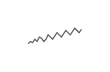
\begin{tikzpicture}[x=0.08em, y=0.08em, line width=0.4pt]
				\draw[FooterGray] (0,3) -- (1,4) -- (2,3.5) -- (3,5) -- (4,4) -- (5,6) -- (6,5.5) -- (7,4) -- (8,5) -- (9,7) -- (10,6) -- (11,5) -- (12,6.5) -- (13,8) -- (14,7) -- (15,6) -- (16,7.5) -- (17,9) -- (18,8) -- (19,7) -- (20,8.5) -- (21,10) -- (22,9) -- (23,8) -- (24,9.5);
			\end{tikzpicture}%
		}%
		\hskip0.5cm%
	}%
	\vskip6pt%
}

%=============================================================================
% COMANDA QUANTLET
%=============================================================================
\newcommand{\quantlet}[2]{%
	\hfill\href{#2}{%
		\raisebox{-0.15em}{
\includegraphics[height=0.7em]{ql_logo.png}}%
		\textcolor{MainBlue}{\tiny\ #1}%
	}%
}

%=============================================================================
% PAGINĂ TITLU PERSONALIZATĂ
%=============================================================================
\defbeamertemplate*{title page}{hybrid}[1][]
{
	\vspace{0.2cm}
	\noindent\makebox[\linewidth][s]{%
		\href{https://www.ase.ro}{
\includegraphics[height=1.0cm]{ase_logo.png}}\hfill%
		\href{https://theida.net}{
\includegraphics[height=1.0cm]{ida_logo.png}}\hfill%
		\href{https://blockchain-research-center.com}{
\includegraphics[height=1.0cm]{brc_logo.png}}\hfill%
		\href{https://www.ai4efin.ase.ro}{
\includegraphics[height=1.0cm]{ai4efin_logo.png}}\hfill%
		\href{https://ipe.ro/new}{
\includegraphics[height=1.0cm]{acad_logo.png}}\hfill%
		\href{https://www.digital-finance-msca.com}{
\includegraphics[height=1.0cm]{msca_logo.png}}%
	}
	\vspace{0.6cm}
	
	\noindent\makebox[\linewidth][c]{%
		\begin{minipage}{0.11\linewidth}
			\centering
			\href{https://quantlet.com}{
\includegraphics[height=1.1cm]{ql_logo.png}}
		\end{minipage}%
		\begin{minipage}{0.76\linewidth}
			\centering
			{\LARGE\bfseries\usebeamercolor[fg]{title}\inserttitle}
			
			\vspace{0.3cm}
			
			{\usebeamerfont{subtitle}\usebeamercolor[fg]{title}\insertsubtitle}
		\end{minipage}%
		\begin{minipage}{0.11\linewidth}
			\centering
			\href{https://quantinar.com}{
\includegraphics[height=1.1cm]{qr_logo.png}}
		\end{minipage}%
	}
	
	\vspace{0.6cm}
	
	\hspace{0.5cm}{\usebeamerfont{author}\insertauthor}
	
	\vspace{0.3cm}
	
	\hspace{0.5cm}\begin{minipage}[t]{0.9\textwidth}
		\raggedright\small\insertinstitute
	\end{minipage}
}
\setbeamertemplate{title page}[hybrid]

%=============================================================================
% MEDII PENTRU TEOREME
%=============================================================================
\theoremstyle{definition}
\setbeamertemplate{theorems}[numbered]
\newtheorem{defn}{Definiție}
\newtheorem{thm}{Teoremă}
\newtheorem{prop}{Propoziție}
\newtheorem{rmk}{Observație}

%=============================================================================
% CENTRED MINIPAGE
%=============================================================================
\newenvironment{cminipage}[1]{%
	\par\noindent\hfill\begin{minipage}{#1}\ignorespaces
	}{%
	\end{minipage}\hfill\null\par
}

%=============================================================================
% COMENZI PERSONALIZATE
%=============================================================================
\newcommand{\E}{\mathbb{E}}
\newcommand{\Var}{\text{Var}}
\newcommand{\Cov}{\text{Cov}}
\newcommand{\Corr}{\text{Corr}}
\newcommand{\VaR}{\text{VaR}}
\newcommand{\ES}{\text{ES}}
\newcommand{\R}{\mathbb{R}}
\newcommand{\N}{\mathbb{N}}
\newcommand{\Z}{\mathbb{Z}}
\newcommand{\B}{\mathbf{B}}
\newcommand{\imark}{\textcolor{MainBlue}{\textbullet}}
\newcommand{\RMSE}{\text{RMSE}}
\newcommand{\MAE}{\text{MAE}}
\newcommand{\MAPE}{\text{MAPE}}
\newcommand{\correct}{\textcolor{Forest}{\checkmark}}
\newcommand{\incorrect}{\textcolor{Crimson}{\texttimes}}

%=============================================================================
% INFORMAȚII TITLU
%=============================================================================
\title[Statistica Piețelor Financiare]{Statistica Piețelor Financiare}
\author[D.T. Pele, A. Amza]{\texorpdfstring{\begin{tabular}[t]{@{}l@{}}Daniel Traian PELE \\ Antoaneta Amza\end{tabular}}{Daniel Traian PELE, Antoaneta Amza}}
\institute{Academia de Studii Economice din București\\
	IDA Institute Digital Assets\\
	Blockchain Research Center\\
	AI4EFin Artificial Intelligence for Energy Finance\\
	Academia Română, Institutul de Prognoză Economică\\
	MSCA Digital Finance}
\date{}
\subtitle{Seminar FMH --- Ipoteza Pieței Fractale (Fractal Market Hypothesis)}

\begin{document}

%=============================================================================
% PAGINA DE TITLU
%=============================================================================
{
\setbeamertemplate{headline}{}
\setbeamertemplate{footline}{}
\begin{frame}
    \titlepage
\end{frame}
}

%=============================================================================
% CUPRINS
%=============================================================================
\begin{frame}[shrink=15]{Cuprins}
\begin{cminipage}{0.95\textwidth}
\begin{columns}[T]
\begin{column}{0.48\textwidth}
\begin{itemize}\setlength{\itemsep}{0pt}
    \item Partea I: Recap teoretic FMH
    \begin{itemize}\setlength{\itemsep}{0pt}
        \item EMH vs FMH; cei 3 piloni Peters
        \item Orizonturi multiple, $D=2-H$
    \end{itemize}
    \item Partea II: Geometrie fractală
    \begin{itemize}\setlength{\itemsep}{0pt}
        \item Cantor, Koch, Sierpinski; box-counting
        \item Coasta Britaniei, self-similarity
    \end{itemize}
    \item Partea III: Estimare $\hat H$
    \begin{itemize}\setlength{\itemsep}{0pt}
        \item Hurst la Nilul; R/S, Lo (1991), DFA, MFDFA
        \item Limitări și combo recomandat
    \end{itemize}
    \item Partea IV: Hurst aplicat
    \begin{itemize}\setlength{\itemsep}{0pt}
        \item SPY, BTC, BET, FX --- diagnostic
    \end{itemize}
\end{itemize}
\end{column}
\begin{column}{0.48\textwidth}
\begin{itemize}\setlength{\itemsep}{0pt}
    \item Partea V: fBm și multifractalitate
    \begin{itemize}\setlength{\itemsep}{0pt}
        \item Wiener vs Mandelbrot--Van~Ness
        \item ARFIMA, MMAR, $f(\alpha)$
    \end{itemize}
    \item Partea VI: Managementul riscului sub FMH
    \begin{itemize}\setlength{\itemsep}{0pt}
        \item VaR cu $T^H$; FIGARCH; rough volatility
    \end{itemize}
    \item Partea VII: Studii de caz --- crize
    \begin{itemize}\setlength{\itemsep}{0pt}
        \item 1987, 2008, COVID; BVB, Bitcoin
    \end{itemize}
    \item Partea VIII: Exerciții de examen
    \item A/F rapid + concluzii + bibliografie
\end{itemize}
\end{column}
\end{columns}
\end{cminipage}
\end{frame}

%=============================================================================
% OBIECTIVE
%=============================================================================
\begin{frame}[shrink=15]{Obiective de învățare}
\begin{cminipage}{0.95\textwidth}
\begin{block}{La finalul seminarului veți putea:}
\begin{itemize}\setlength{\itemsep}{0pt}
    \item Defini FMH și cei 3 piloni Peters (1991, 1994); deosebi FMH de EMH
    \item Calcula dimensiunea fractală pentru obiecte autosimilare (Cantor, Koch, Sierpinski) și estima box-counting empiric
    \item Aplica algoritmul R/S pas-cu-pas; cunoaște corecția Lo (1991) și DFA
    \item Interpreta $\hat H$ pe active reale (acțiuni, cripto, FX, BVB) și recunoaște capcanele de interpretare
    \item Defini fBm formal (Mandelbrot--Van~Ness 1968) și conexiunea cu ARFIMA
    \item Discuta multifractalitatea, MMAR și spectrul $f(\alpha)$
    \item Compara VaR scalat cu $\sqrt T$ vs $T^H$ ca exercițiu de \textbf{analiză de sensibilitate} și de testare la stres sub memorie lungă (\textbf{nu} ca substitut pentru cadrul Basel)
    \item Folosi $\hat H_t$ mobil ca \textbf{semnal de avertizare timpurie} pentru crize: 1987, 2008, COVID-19
\end{itemize}
\end{block}
\end{cminipage}
\end{frame}

%=============================================================================
% ROADMAP PEDAGOGIC
%=============================================================================
\begin{frame}[shrink=15]{Roadmap pedagogic --- 5 pași}
\begin{cminipage}{0.95\textwidth}
\begin{block}{Drumul de la EMH la FMH în acest seminar}
\begin{enumerate}\setlength{\itemsep}{4pt}
    \item \textbf{Limitele etalonului EMH / mers aleator}: ce nu poate explica un benchmark gaussian, i.i.d., cu agent reprezentativ (cozi grele, memorie, crize)
    \item \textbf{Ideea de scalare și fractali}: autosimilaritate statistică, dimensiune fractală, geometria piețelor
    \item \textbf{Estimarea exponentului Hurst}: R/S, DFA, MFDFA --- cum citim memoria pieței din date
    \item \textbf{Aplicații pe piețe reale}: SPY, BTC, BVB, FX --- ce ne spune $\hat H$ despre eficiență
    \item \textbf{Implicații pentru risc și crize}: scalarea VaR, $T^H$ ca diagnostic de stres, $\hat H_t$ ca semnal de regim în 1987, 2008, COVID
\end{enumerate}
\end{block}
\begin{exampleblock}{Trei tipuri de slide-uri}
\begin{itemize}\setlength{\itemsep}{0pt}
    \item \textbf{CORE SEMINAR} --- conținutul principal (parțile I--VII)
    \item \textbf{EXERCIȚII} --- mini-exerciții și probleme de examen (partea VIII)
    \item \textbf{APPENDIX OPȚIONAL} --- glosar extins, demonstrații avansate, modele tehnice (anexe A--C)
\end{itemize}
\end{exampleblock}
\end{cminipage}
\end{frame}

%=============================================================================
% MINI-GLOSAR (DOAR ACRONIMELE FOLOSITE IMEDIAT)
%=============================================================================
\begin{frame}[shrink=15]{Mini-glosar: acronimele utilizate frecvent}
\begin{cminipage}{0.95\textwidth}
\begin{block}{Cele 9 acronime de care ai nevoie pentru parțile I--III}
\begin{itemize}\setlength{\itemsep}{1pt}
    \item \textbf{EMH} --- Ipoteza Pieței Eficiente (\textit{Efficient Market Hypothesis})
    \item \textbf{FMH} --- Ipoteza Pieței Fractale (\textit{Fractal Market Hypothesis})
    \item \textbf{fBm / fGn} --- mișcare browniană / zgomot gaussian fracționar
    \item \textbf{R/S} --- scalarea reescalată (\textit{Rescaled Range}; Hurst 1951)
    \item \textbf{DFA} --- analiza fluctuațiilor cu eliminarea trendului
    \item \textbf{VaR / ES} --- valoarea la risc / pierderea așteptată
    \item \textbf{BVB / BET} --- Bursa de Valori București și indicele său
\end{itemize}
\end{block}
\begin{exampleblock}{Glosar complet}
\begin{itemize}\setlength{\itemsep}{0pt}
    \item Restul acronimelor (AMH, ARFIMA, GARCH, FIGARCH, HAR, MMAR, MSM, MFDFA, GPH, WTMM, HFT, FRTB, LULD, GFC, ACF, OLS etc.) sunt definite la prima utilizare și recapitulate în \textbf{Anexa A0}
\end{itemize}
\end{exampleblock}
\end{cminipage}
\end{frame}

%#############################################################################
\section{Partea I: Recap teoretic FMH [CORE]}
%#############################################################################

\begin{frame}[shrink=15]{Fapte stilizate ale randamentelor financiare (recap Cap.~2--4)}
\begin{cminipage}{0.95\textwidth}
\begin{block}{Cele 5 fapte principale}
\begin{enumerate}\setlength{\itemsep}{2pt}
    \item Distribuții cu \textbf{cozi grele} (kurtoză $>3$)
    \item Randamente \textbf{aproape necorelate} pe lag pozitiv: $\rho(r_t,r_{t+k})\approx 0$
    \item \textbf{Aglomerarea volatilității}: $|r_t|, r_t^2$ puternic autocorelate
    \item \textbf{Memorie lungă în volatilitate}: $\rho(r_t^2,r_{t+k}^2)\sim k^{-\beta}$
    \item \textbf{Efectul de levier}: $\Corr(r_t, r_{t+k}^2)<0$ pentru $k>0$
\end{enumerate}
\end{block}
\begin{exampleblock}{Care cadru acoperă ce}
\begin{itemize}\setlength{\itemsep}{0pt}
    \item \textbf{EMH + mers aleator gaussian}: doar (2) parțial; eșuează pe (1), (3), (4)
    \item \textbf{Distribuții stabile}: acoperă (1); nu și (3), (4)
    \item \textbf{FMH / MMAR}: cadru unificat pentru (1), (3), (4) și pentru memoria în randamente
\end{itemize}
\end{exampleblock}
\begin{alertblock}{Notă}
\begin{itemize}\setlength{\itemsep}{0pt}
    \item Fapte suplimentare omise aici: \textbf{asimetrie negativă} ($\E[r^3]<0$) și \textbf{gaussianitate prin agregare}
    \item ,,EMH'' = etalonul random-walk gaussian i.i.d.; EMH modernă (Fama 1991, 2014) nu impune nici gaussianitate, nici identitate de orizonturi
\end{itemize}
\end{alertblock}
\end{cminipage}
\end{frame}

\begin{frame}[shrink=15]{De ce avem nevoie de o abordare nouă?}
\begin{cminipage}{0.95\textwidth}
\begin{columns}[T]
\begin{column}{0.55\textwidth}
\begin{itemize}\setlength{\itemsep}{0pt}
    \item \textbf{Eșecuri empirice ale EMH} (Cap.~4):
    \begin{itemize}\setlength{\itemsep}{0pt}
        \item Cozi grele: $\Pr(|r_t|>x)\gg\Phi(-x)$
        \item Aglomerarea volatilității: $\Corr(|r_t|,|r_{t+k}|)>0$
        \item Memorie lungă: $\rho(k)\sim Ck^{2H-2}$, $H>0{,}5$
        \item Crahuri: 1987, 2008, COVID-2020
    \end{itemize}
    \item Sub gaussianitate: $\Pr(r\leq -22{,}6\%)\approx 10^{-50}$
    \item Mandelbrot (1963): randamentele zilnice ale bumbacului sunt \textbf{compatibile cu o lege $\alpha$-stabilă cu $\alpha<2$} (varianță teoretică infinită)
\end{itemize}
\end{column}
\begin{column}{0.42\textwidth}
\centering
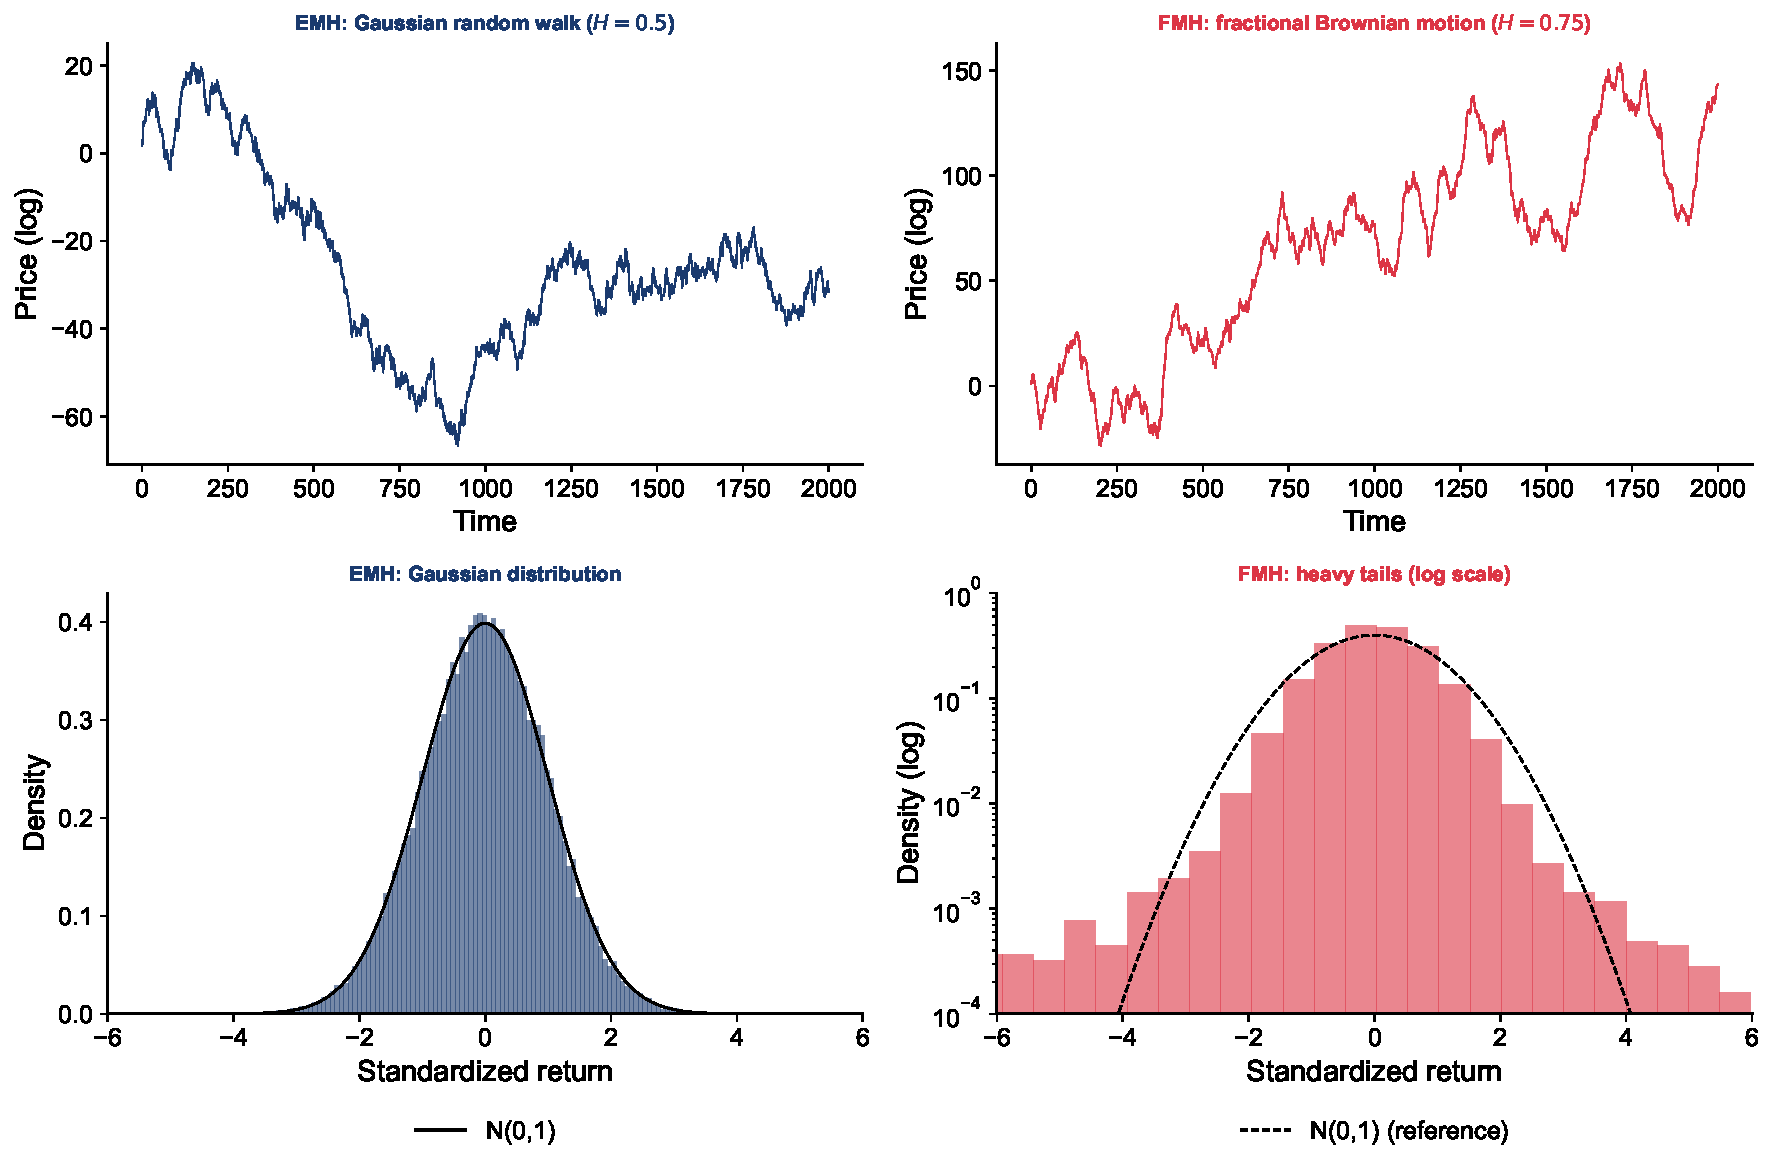
\includegraphics[width=\linewidth]{ch_fmh_emh_vs_fmh.pdf}\\[1pt]
{\scriptsize\textcolor{MediumGray}{\textit{Etalon EMH (mers aleator gaussian) vs ilustrație FMH (fBm cu $H=0{,}75$). Aici se vede doar memoria/scalarea --- cozile grele provin separat din distribuții stabile, MMAR sau schimbare de timp (time change).}}}
\end{column}
\end{columns}
\quantlet{SFM\_ch\_fmh\_fractals: emh\_vs\_fmh}{https://github.com/danpele/SFM/tree/main/Quantlets/SFM_ch_fmh}
\end{cminipage}
\end{frame}

\begin{frame}[shrink=15]{Anomalii care contrazic EMH}
\begin{cminipage}{0.95\textwidth}
\renewcommand{\arraystretch}{1.2}
\begin{center}
\small
\begin{tabular}{ll}
\toprule
\textbf{Anomalie} & \textbf{Predicție EMH} \\
\midrule
Cozi grele & Imposibil sub gaussianitate \\
Aglomerarea volatilității & Independență $\Rightarrow$ corelație 0 \\
Memorie lungă, $\rho(k)\sim k^{2H-2}$, $H>0{,}5$ & $\rho(k)=0$ pentru $k>0$ \\
Momentum (3--12 luni) & Imposibil sub mers aleator \\
Reversal (3--5 ani) & Imposibil sub independență \\
Post-Earnings Announcement Drift (PEAD) & Reflectare instantanee \\
Black Monday 1987 ($-22{,}6\%$) & Probabilitate $\sim 10^{-50}$ \\
Bule (DotCom 2000, cripto 2017, 2021) & Excluse de raționalitate \\
\bottomrule
\end{tabular}
\end{center}
\vspace{0.15cm}
\begin{itemize}\setlength{\itemsep}{0pt}
    \item Toate aceste fenomene au în comun \textbf{scalare aproximativă, dependență temporală, cozi grele; posibil $H\neq 0{,}5$}
    \item EMH e utilă, dar incompletă $\Rightarrow$ nevoie de un cadru \textit{fractal}
\end{itemize}
\end{cminipage}
\end{frame}

\begin{frame}[shrink=15]{Răspunsul FMH (Peters, 1991, 1994)}
\begin{cminipage}{0.95\textwidth}
\begin{block}{Trei principii FMH}
\begin{itemize}\setlength{\itemsep}{2pt}
    \item Piețele sunt sisteme \textbf{fractale}: structură statistică similară pe scale temporale diferite
    \item Investitorii operează pe \textbf{orizonturi multiple}: de la milisecunde (tranzacționare de înaltă frecvență --- HFT, \textit{High-Frequency Trading}) la decenii (pensii)
    \item Stabilitatea $\Leftrightarrow$ \textbf{diversitatea} orizonturilor; colapsul lor $\Rightarrow$ criză
\end{itemize}
\end{block}
\begin{exampleblock}{Mini-glosar --- fBm}
\begin{itemize}\setlength{\itemsep}{0pt}
    \item fBm (\textit{fractional Brownian motion}) = mișcare browniană fracționară (Mandelbrot \& Van~Ness, 1968)
    \item Generalizare a mișcării browniene cu memorie reglată de $H$
    \item $H=0{,}5$ recuperează mișcarea browniană standard
\end{itemize}
\end{exampleblock}
\begin{itemize}\setlength{\itemsep}{0pt}
    \item Cărțile fundamentale: Peters (1991) \textit{Chaos and Order in the Capital Markets}; Peters (1994) \textit{Fractal Market Analysis}
\end{itemize}
\end{cminipage}
\end{frame}

\begin{frame}[shrink=15]{De la geometria euclidiană la fractali}
\begin{cminipage}{0.95\textwidth}
\begin{columns}[T]
\begin{column}{0.50\textwidth}
\begin{block}{Geometria euclidiană}
\begin{itemize}\setlength{\itemsep}{0pt}
    \item Forme regulate, netede (drepte, cercuri, sfere)
    \item Dimensiune $D\in\{0,1,2,3\}$ (întregi)
\end{itemize}
\end{block}
\begin{block}{Geometria fractală (Mandelbrot, 1975)}
\begin{itemize}\setlength{\itemsep}{0pt}
    \item Forme neregulate, fragmentate, autosimilare
    \item Țărmuri, nori, copaci, randamente
    \item Dimensiune $D\in\R$ (fracționară)
\end{itemize}
\end{block}
\end{column}
\begin{column}{0.46\textwidth}
\begin{alertblock}{Citat (Mandelbrot, 1982)}
\begin{itemize}\setlength{\itemsep}{0pt}
    \item \textit{,,Norii nu sunt sfere''}
    \item \textit{,,Țărmurile nu sunt cercuri''}
    \item \textit{,,Fulgerul nu călătorește în linie dreaptă''}
    \item \textit{,,Markets are turbulent like fluids and fractal like coastlines.''} (2004)
\end{itemize}
\end{alertblock}
\begin{exampleblock}{Benoît Mandelbrot}
\begin{itemize}\setlength{\itemsep}{0pt}
    \item 1924--2010, IBM Research $\to$ Yale
    \item Părinte al \textbf{geometriei fractale}
\end{itemize}
\end{exampleblock}
\end{column}
\end{columns}
\end{cminipage}
\end{frame}

\begin{frame}[shrink=15]{EMH vs FMH: comparație directă}
\begin{cminipage}{0.95\textwidth}
\begin{columns}[T]
\begin{column}{0.48\textwidth}
\begin{block}{EMH (Fama, 1970)}
\begin{itemize}\setlength{\itemsep}{0pt}
    \item \textbf{Benchmark random-walk / agent reprezentativ}: abstractizează de la heterogenitatea orizonturilor
    \item Informația reflectată \textbf{instantaneu}
    \item Randamente \textbf{i.i.d.}, varianță finită
    \item Mers aleator (Brown), $H=0{,}5$
    \item Scalare $\sigma(\Delta)=\sigma(1)\sqrt{\Delta}$
\end{itemize}
\textit{\footnotesize Notă: EMH modernă (Fama 1991, 2014) nu impune nici gaussianitate, nici identitate de orizonturi.}
\end{block}
\end{column}
\begin{column}{0.48\textwidth}
\begin{alertblock}{FMH (Peters, 1991)}
\begin{itemize}\setlength{\itemsep}{0pt}
    \item Investitori pe \textbf{orizonturi multiple}
    \item Stabilitatea $\propto$ \textbf{diversitatea orizonturilor}
    \item Randamente cu \textbf{autosimilaritate} și memorie
    \item De obicei $H\neq 0{,}5$ (cel mai des $H>0{,}5$)
    \item Scalare $\sigma(\Delta)=\sigma(1)\,\Delta^H$
\end{itemize}
\end{alertblock}
\end{column}
\end{columns}
\vspace{0.2cm}
\begin{exampleblock}{Mecanismul lichidității}
\begin{itemize}\setlength{\itemsep}{0pt}
    \item Traderii pe termen scurt vând $\Rightarrow$ investitorii pe termen lung cumpără $\Rightarrow$ \textbf{lichiditate}
    \item Cu orizonturi omogene, lichiditatea \textbf{dispare}
\end{itemize}
\end{exampleblock}
\end{cminipage}
\end{frame}

\begin{frame}[shrink=15]{Orizonturi multiple: cele 5 cohorte}
\begin{cminipage}{0.95\textwidth}
\begin{columns}[T]
\begin{column}{0.55\textwidth}
\begin{itemize}\setlength{\itemsep}{1pt}
    \item Cinci cohorte tipice de investitori:
    \begin{itemize}\setlength{\itemsep}{0pt}
        \item Tranzacționare de înaltă frecvență (HFT): milisecunde--minute
        \item Tranzacționare intra-zi: ore--zile
        \item Speculație pe poziție (swing): săptămâni--luni
        \item Fonduri de hedging: luni--ani
        \item Fonduri de pensii și suverane: ani--decenii
    \end{itemize}
    \item \textbf{Diversitate de orizonturi} = răspândirea ponderilor pe cohortele de mai sus
    \item \textbf{Colapsul orizonturilor} = ponderile se concentrează pe o singură cohortă (de regulă cea scurtă)
\end{itemize}
\end{column}
\begin{column}{0.42\textwidth}
\begin{exampleblock}{Proxy didactic: entropia orizonturilor}
\begin{itemize}\setlength{\itemsep}{0pt}
    \item $\mathcal{H}_{\text{horiz}}=-\sum_i w_i\log w_i$
    \item Mare $\Leftrightarrow$ orizonturi diverse
    \item Mic $\Leftrightarrow$ concentrare $\Leftrightarrow$ criză
    \item \textbf{Nu este o lege formală}, ci ilustrație didactică
\end{itemize}
\end{exampleblock}
\end{column}
\end{columns}
\end{cminipage}
\end{frame}

\begin{frame}[shrink=15]{Crahuri ca colaps al orizonturilor}
\begin{cminipage}{0.95\textwidth}
\begin{block}{Naratorul informal (FMH)}
\begin{itemize}\setlength{\itemsep}{2pt}
    \item Un \textbf{șoc fundamental} (Lehman, COVID) afectează simultan toate orizonturile
    \item Investitorii pe termen lung adoptă comportament pe termen scurt (vânzare în panică)
    \item Distribuția orizonturilor \textbf{colapsează} $\Rightarrow$ \textbf{lichiditatea dispare}
    \item Structura fractală se rupe $\Rightarrow$ $\hat{H}_t$ se schimbă brusc
\end{itemize}
\end{block}
\begin{exampleblock}{Evidență}
\begin{itemize}\setlength{\itemsep}{0pt}
    \item Criza 2008: $\hat{H}_t$ pe S\&P~500 a scăzut spre $0{,}5$ (Dominique \& Rivera, 2011)
    \item COVID martie 2020: colaps al diversității în câteva zile, $\hat{H}_t$ atinge $\sim 0{,}40$
    \item Black Monday (1987): asigurare de portofoliu $+$ tranzacționare programată $\Rightarrow$ omogenizare
\end{itemize}
\end{exampleblock}
\end{cminipage}
\end{frame}

\begin{frame}[shrink=15]{De la mers aleator (Bachelier 1900) la fractali (Mandelbrot 1963)}
\begin{cminipage}{0.95\textwidth}
\begin{columns}[T]
\begin{column}{0.50\textwidth}
\begin{block}{Bachelier (1900)}
\begin{itemize}\setlength{\itemsep}{0pt}
    \item Teză de doctorat: ,,Théorie de la spéculation''
    \item $\Delta P\sim\mathcal{N}(0,\sigma^2\Delta t)$
    \item Implicit $H=0{,}5$
    \item Forma \textbf{netedă} statistic
    \item Bază pentru Black--Scholes (1973)
\end{itemize}
\end{block}
\end{column}
\begin{column}{0.46\textwidth}
\begin{alertblock}{Mandelbrot (1963, 1967)}
\begin{itemize}\setlength{\itemsep}{0pt}
    \item ,,The variation of certain speculative prices'' (\textit{J.\ Business}, 36)
    \item Bumbac: \textbf{randamentele zilnice} sunt compatibile cu o lege $\alpha$-stabilă cu $\alpha<2$ (varianță teoretică infinită)
    \item Dimensiunea graficului prețului: $D\approx 2-H$ (sub fBm)
    \item Indici reali: $D\in[1{,}3;\,1{,}5]$ $\Rightarrow$ \textbf{nu} mers aleator pur
    \item Mandelbrot \& Wallis (1969): R/S pe finanțe
\end{itemize}
\end{alertblock}
\end{column}
\end{columns}
\vspace{0.1cm}
\centering
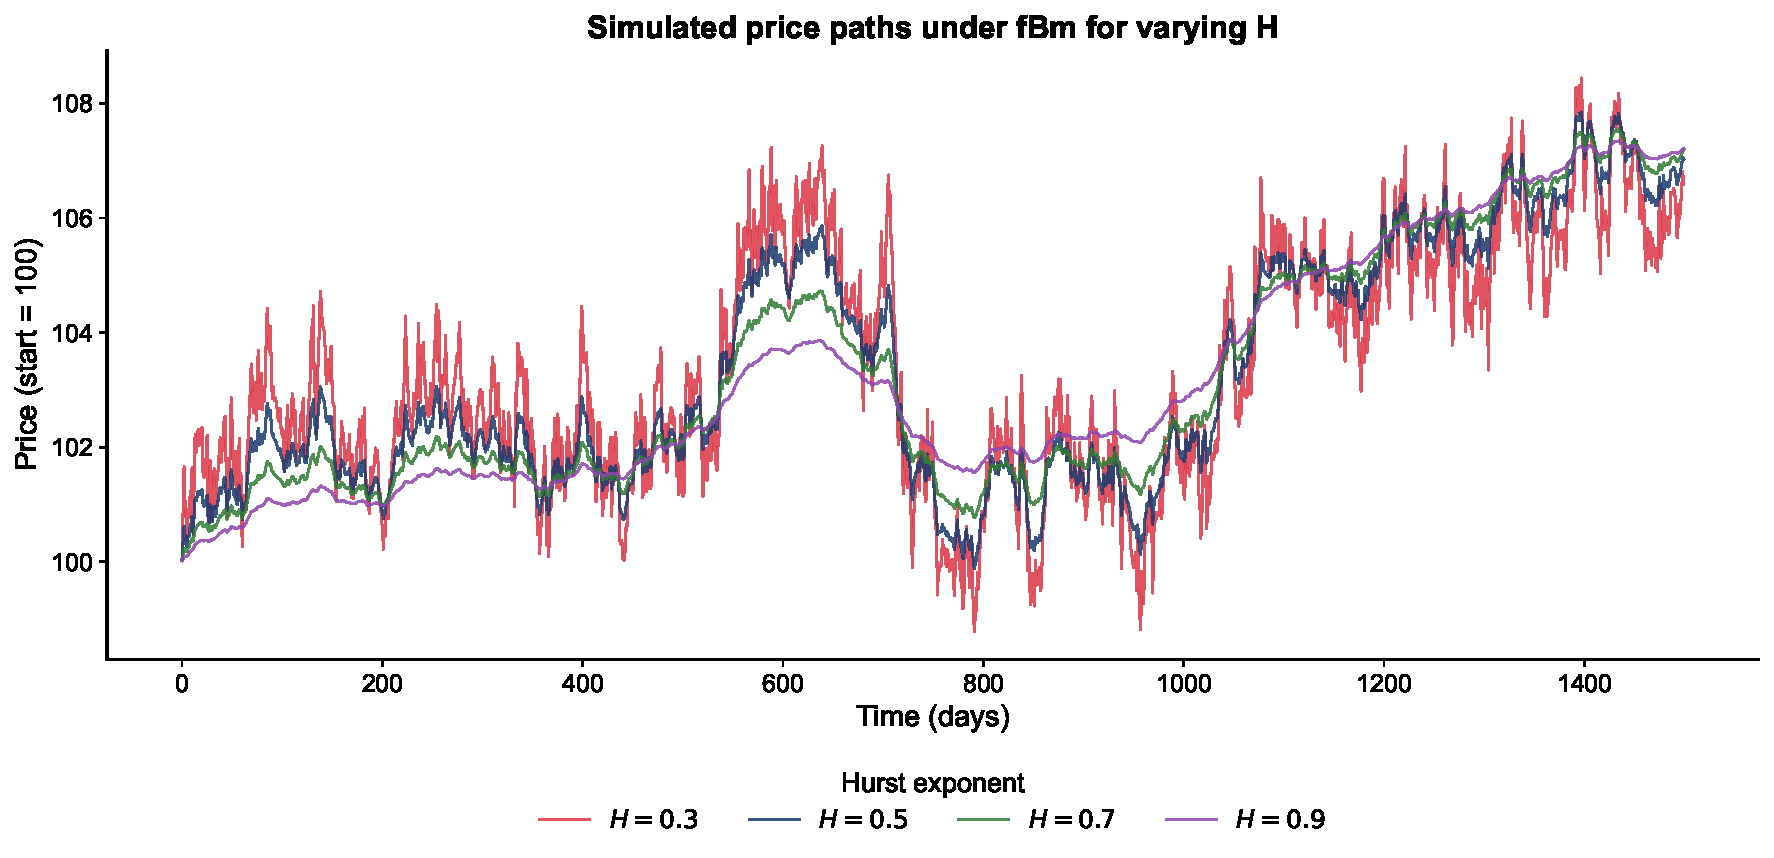
\includegraphics[width=0.65\linewidth,height=2.6cm,keepaspectratio]{ch_fmh_price_paths_H.pdf}
\end{cminipage}
\end{frame}

\begin{frame}[shrink=15]{Imaginea centrală: traiectorii și self-similarity}
\begin{cminipage}{0.95\textwidth}
\begin{columns}[T]
\begin{column}{0.48\textwidth}
\centering
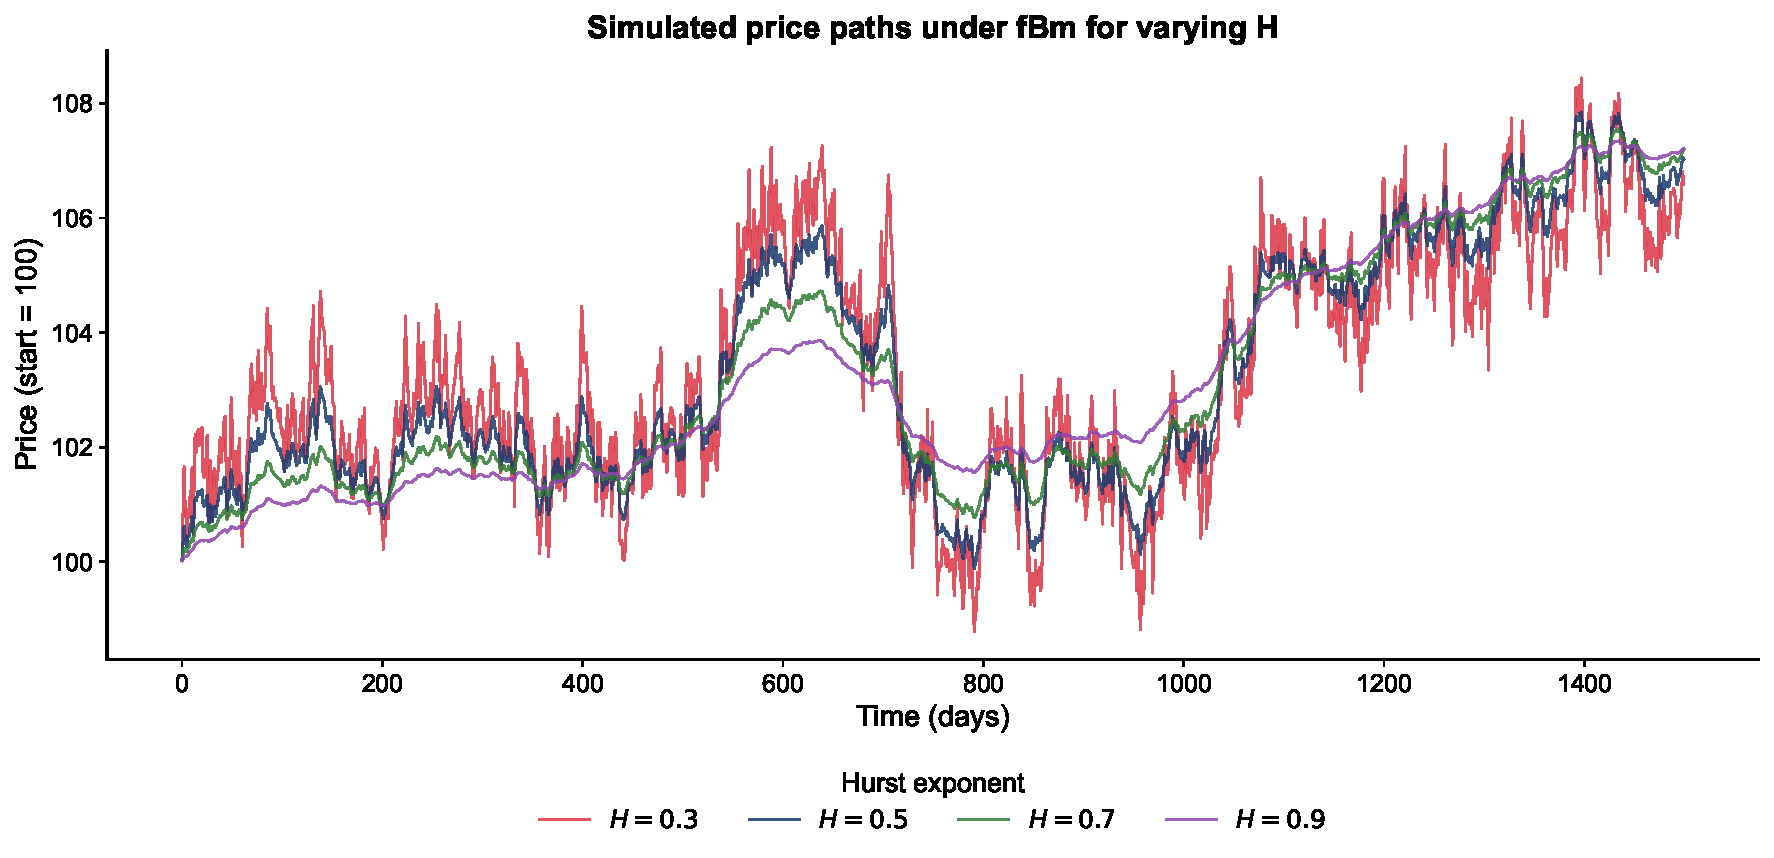
\includegraphics[width=\linewidth]{ch_fmh_price_paths_H.pdf}\\[1pt]
{\scriptsize\textcolor{MediumGray}{\textit{Patru traiectorii pentru valori diferite ale $H$.}}}
\end{column}
\begin{column}{0.48\textwidth}
\centering
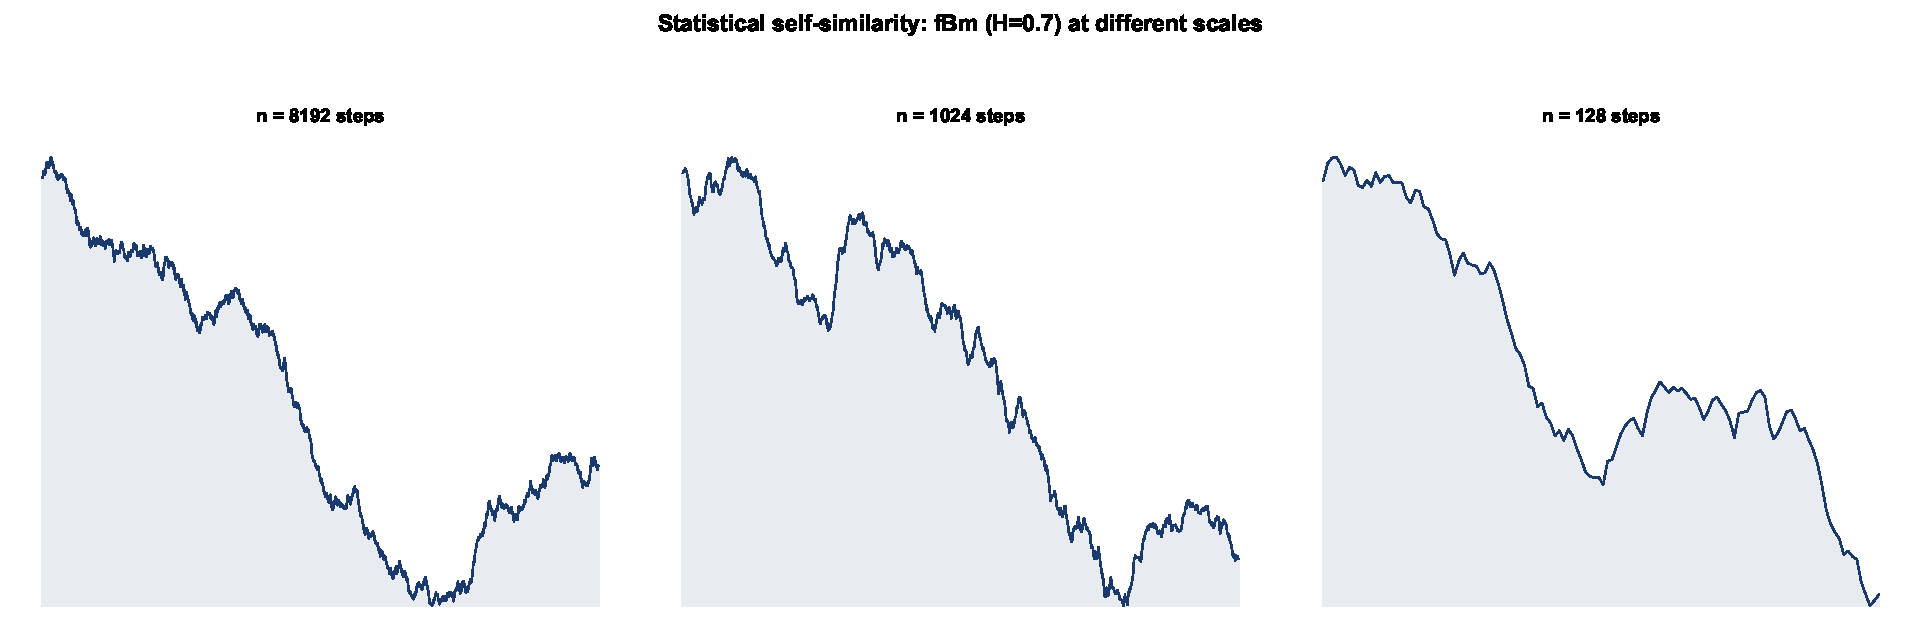
\includegraphics[width=\linewidth]{ch_fmh_selfsimilarity.pdf}\\[1pt]
{\scriptsize\textcolor{MediumGray}{\textit{Aceeași traiectorie fBm la trei nivele de zoom.}}}
\end{column}
\end{columns}
\vspace{0.1cm}
\begin{itemize}\setlength{\itemsep}{0pt}
    \item $H<0{,}5$: traiectorii zimțate, mean-reverting (anti-persistență)
    \item $H=0{,}5$: random walk standard (regula $\sqrt T$)
    \item $H>0{,}5$: traiectorii netede, persistente (memorie lungă)
    \item \textbf{Autosimilaritate statistică}: structura se conservă la zoom
\end{itemize}
\quantlet{SFM\_ch\_fmh\_fractals: price\_paths\_H, selfsimilarity}{https://github.com/danpele/SFM/tree/main/Quantlets/SFM_ch_fmh}
\end{cminipage}
\end{frame}

\begin{frame}[shrink=15]{Recap §I: 3 idei-cheie}
\begin{cminipage}{0.95\textwidth}
\begin{block}{De reținut}
\begin{enumerate}\setlength{\itemsep}{4pt}
    \item EMH (Cap.~4) e utilă, dar incompletă: nu explică cozile grele, aglomerarea volatilității, memoria lungă și crahurile
    \item FMH propune \textbf{piețe fractale + orizonturi multiple}; stabilitatea piețelor depinde de \textbf{diversitatea orizonturilor}
    \item Crahurile = \textbf{colapsul} acestei diversități; schimbări bruște ale $\hat{H}_t$ (scăderi spre/sub $0{,}5$ sau creșteri persistente) pot semnala schimbarea de regim, validată cu robustețe și sub-eșantioane
\end{enumerate}
\end{block}
\begin{exampleblock}{Tranziție: \textit{,,acum trecem de la motivație la geometrie''}}
\begin{itemize}\setlength{\itemsep}{0pt}
    \item §II: măsurăm ,,cât de neregulat'' este un obiect $\Rightarrow$ \textbf{dimensiunea fractală}
    \item §III: aplicăm pe randamente $\Rightarrow$ \textbf{exponentul Hurst}
\end{itemize}
\end{exampleblock}
\end{cminipage}
\end{frame}

%#############################################################################
\section{Partea II: Geometrie fractală [CORE]}
%#############################################################################

\begin{frame}[shrink=15]{Dimensiunea de similaritate: $D=\log N/\log s$}
\begin{cminipage}{0.95\textwidth}
\begin{block}{Definiție (autosimilaritate exactă)}
\begin{itemize}\setlength{\itemsep}{0pt}
    \item Obiect autosimilar $\to$ $N$ copii la scara $r=1/s$
    \item $\boxed{\,D=\dfrac{\log N}{\log s}=\dfrac{\log N}{\log(1/r)}\,}$
\end{itemize}
\end{block}
\begin{columns}[T]
\begin{column}{0.48\textwidth}
\begin{exampleblock}{Sanity check (cazuri întregi)}
\begin{itemize}\setlength{\itemsep}{0pt}
    \item Linie: $N=2$, $r=1/2 \Rightarrow D=\log 2/\log 2=1$
    \item Pătrat: $N=4$, $r=1/2 \Rightarrow D=\log 4/\log 2=2$
    \item Cub: $N=8$, $r=1/2 \Rightarrow D=\log 8/\log 2=3$
\end{itemize}
\end{exampleblock}
\end{column}
\begin{column}{0.48\textwidth}
\begin{alertblock}{Cazuri fractale}
\begin{itemize}\setlength{\itemsep}{0pt}
    \item Cantor: $D=\log 2/\log 3\approx 0{,}631$
    \item Koch: $D=\log 4/\log 3\approx 1{,}262$
    \item Sierpinski triangle: $D=\log 3/\log 2\approx 1{,}585$
    \item Sierpinski carpet: $D=\log 8/\log 3\approx 1{,}893$
\end{itemize}
\end{alertblock}
\end{column}
\end{columns}
\vspace{0.1cm}
\begin{exampleblock}{Cheie pentru piețe}
\begin{itemize}\setlength{\itemsep}{0pt}
    \item Pentru procese self-affine de tip fBm, dimensiunea graficului este aproximativ $D\approx 2-H$ (Mandelbrot 1968)
    \item În date financiare reale: \textbf{aproximație diagnostică}, nu identitate universală
    \item $D$ măsoară cât de neregulat este graficul prețului
\end{itemize}
\end{exampleblock}
\end{cminipage}
\end{frame}

\begin{frame}[shrink=15]{Mulțimea Cantor: primul fractal modern}
\begin{cminipage}{0.95\textwidth}
\begin{columns}[T]
\begin{column}{0.48\textwidth}
\begin{defn}[Mulțimea Cantor]
Pornind de la $C_0=[0,1]$, la fiecare pas se elimină \textbf{treimea de mijloc} a fiecărui interval. $C=\bigcap_{k\geq 0} C_k$.
\end{defn}
\begin{itemize}\setlength{\itemsep}{0pt}
    \item Lungime totală $0$, infinitate \textbf{nenumărabilă} de puncte
    \item $N=2$ copii la $r=1/3$
    \item Dimensiune: $D=\log 2/\log 3\approx 0{,}631$
\end{itemize}
\end{column}
\begin{column}{0.48\textwidth}
\centering
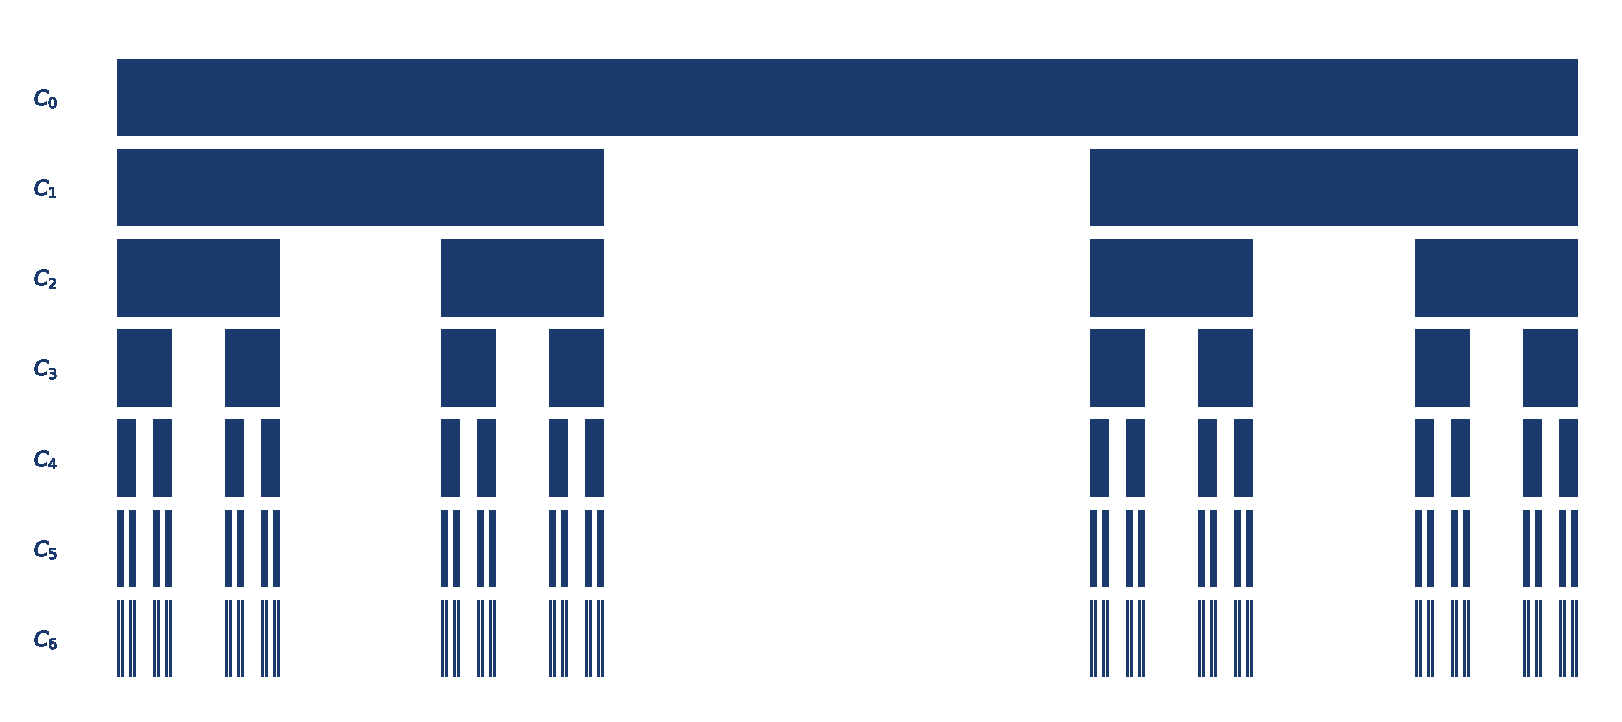
\includegraphics[width=\linewidth]{ch_fmh_cantor.pdf}\\[2pt]
{\scriptsize\textcolor{MediumGray}{\textit{Primele 7 iterații în construcția mulțimii Cantor.}}}
\end{column}
\end{columns}
\vspace{0.1cm}
\begin{exampleblock}{Calcul iterativ pe lungimi}
\begin{itemize}\setlength{\itemsep}{0pt}
    \item $|C_0|=1$, $|C_1|=2/3$, $|C_2|=4/9$, $|C_k|=(2/3)^k\to 0$
    \item Numărul de intervale: $N_k=2^k$; lungimea fiecăruia: $\varepsilon_k=3^{-k}$
    \item Verificăm: $\log N_k/\log(1/\varepsilon_k)=k\log 2/(k\log 3)=\log 2/\log 3$ \checkmark
\end{itemize}
\end{exampleblock}
\quantlet{SFM\_ch\_fmh\_fractals: cantor}{https://github.com/danpele/SFM/tree/main/Quantlets/SFM_ch_fmh}
\end{cminipage}
\end{frame}

\begin{frame}[shrink=25]{Mini-exercițiu A: dimensiunea unui fractal nou}
\begin{cminipage}{0.95\textwidth}
\begin{block}{Sarcină}
\begin{itemize}\setlength{\itemsep}{0pt}
    \item Fie un fractal construit prin: \textbf{$N=5$ copii} la scara \textbf{$r=1/3$}
    \item Calculați $D$ și plasați-l între Cantor ($\log 2/\log 3$) și Koch ($\log 4/\log 3$)
\end{itemize}
\end{block}
\begin{block}{Pași}
\begin{enumerate}\setlength{\itemsep}{0pt}
    \item Aplicați formula de similaritate: $D=\log N/\log(1/r)$
    \item Substituiți $N=5$, $1/r=3$
    \item Evaluați numeric și comparați cu valorile de referință
\end{enumerate}
\end{block}
\begin{exampleblock}{Răspuns}
\begin{itemize}\setlength{\itemsep}{0pt}
    \item $D=\log 5/\log 3\approx \mathbf{1{,}465}$
    \item Mai mare decât Koch ($1{,}262$), mai mic decât Sierpinski triangle ($1{,}585$)
\end{itemize}
\end{exampleblock}
\begin{alertblock}{Interpretare}
\begin{itemize}\setlength{\itemsep}{0pt}
    \item $D$ cuantifică ,,umplerea'' planului: cu cât $N$ crește la aceeași scară $r$, cu atât obiectul e mai dens
    \item Limita: $N=9, r=1/3 \Rightarrow D=2$ --- umple planul, nu mai e fractal
\end{itemize}
\end{alertblock}
\end{cminipage}
\end{frame}

\begin{frame}[shrink=15]{Curba Koch: lungime infinită, arie finită}
\begin{cminipage}{0.96\textwidth}
\begin{columns}[T]
\begin{column}{0.48\textwidth}
\begin{block}{Construcție Koch (1904)}
\begin{itemize}\setlength{\itemsep}{0pt}
    \item Pornim de la un segment de lungime 1
    \item La fiecare iterație fiecare segment $\to$ \textbf{4 segmente} de lungime $1/3$
    \item Lungime la iterația $k$: $L_k=(4/3)^k\to\infty$
    \item Arie limitată (inclusă în triunghi)
\end{itemize}
\end{block}
\begin{exampleblock}{Dimensiune}
\begin{itemize}\setlength{\itemsep}{0pt}
    \item $N=4$, $r=1/3$
    \item $D=\log 4/\log 3\approx \mathbf{1{,}262}$
    \item Mai mult decât o linie, mai puțin decât un plan
\end{itemize}
\end{exampleblock}
\end{column}
\begin{column}{0.48\textwidth}
\centering
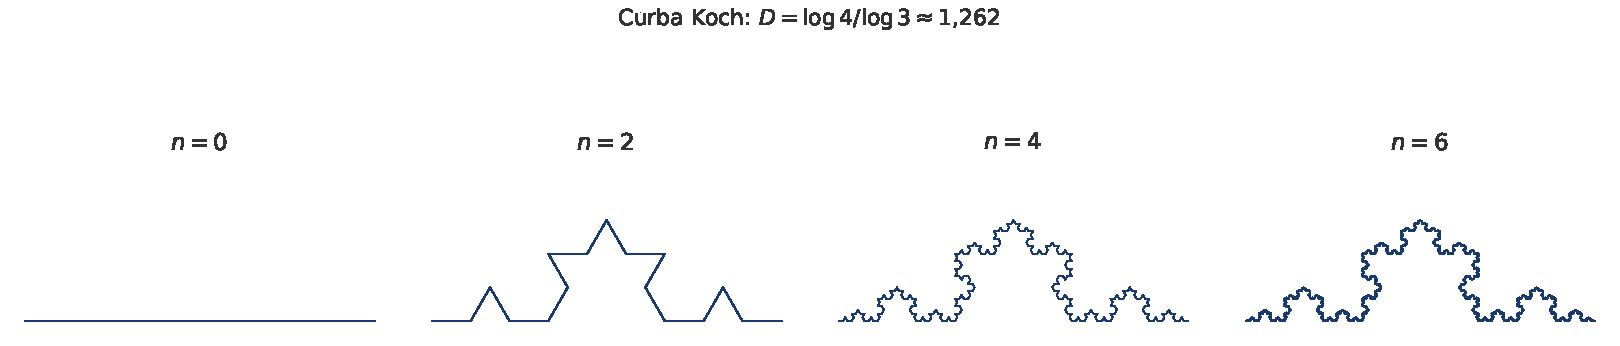
\includegraphics[width=\linewidth,height=4.6cm,keepaspectratio]{ch_fmh_koch_curve.pdf}\\[1pt]
{\scriptsize\textcolor{MediumGray}{\textit{Curba Koch la iterațiile $n=0,2,4,6$.}}}
\end{column}
\end{columns}
\quantlet{SFM\_ch\_fmh\_fractals: koch\_curve}{https://github.com/danpele/SFM/tree/main/Quantlets/SFM_ch_fmh}
\end{cminipage}
\end{frame}

\begin{frame}[shrink=15]{Triunghiul și covorul Sierpinski}
\begin{cminipage}{0.95\textwidth}
\begin{columns}[T]
\begin{column}{0.46\textwidth}
\begin{block}{Sierpinski triangle (1915)}
\begin{itemize}\setlength{\itemsep}{0pt}
    \item Construit prin \textit{chaos game} sau eliminare iterativă
    \item $N=3$ copii la $r=1/2$
    \item $D=\log 3/\log 2\approx 1{,}585$
\end{itemize}
\end{block}
\begin{block}{Sierpinski carpet (covorul)}
\begin{itemize}\setlength{\itemsep}{0pt}
    \item Pătratul unitate $\to 9$ pătrate; eliminăm pătratul central
    \item $N=8$ copii la $r=1/3$
    \item $D=\log 8/\log 3\approx 1{,}893$
\end{itemize}
\end{block}
\end{column}
\begin{column}{0.52\textwidth}
\centering
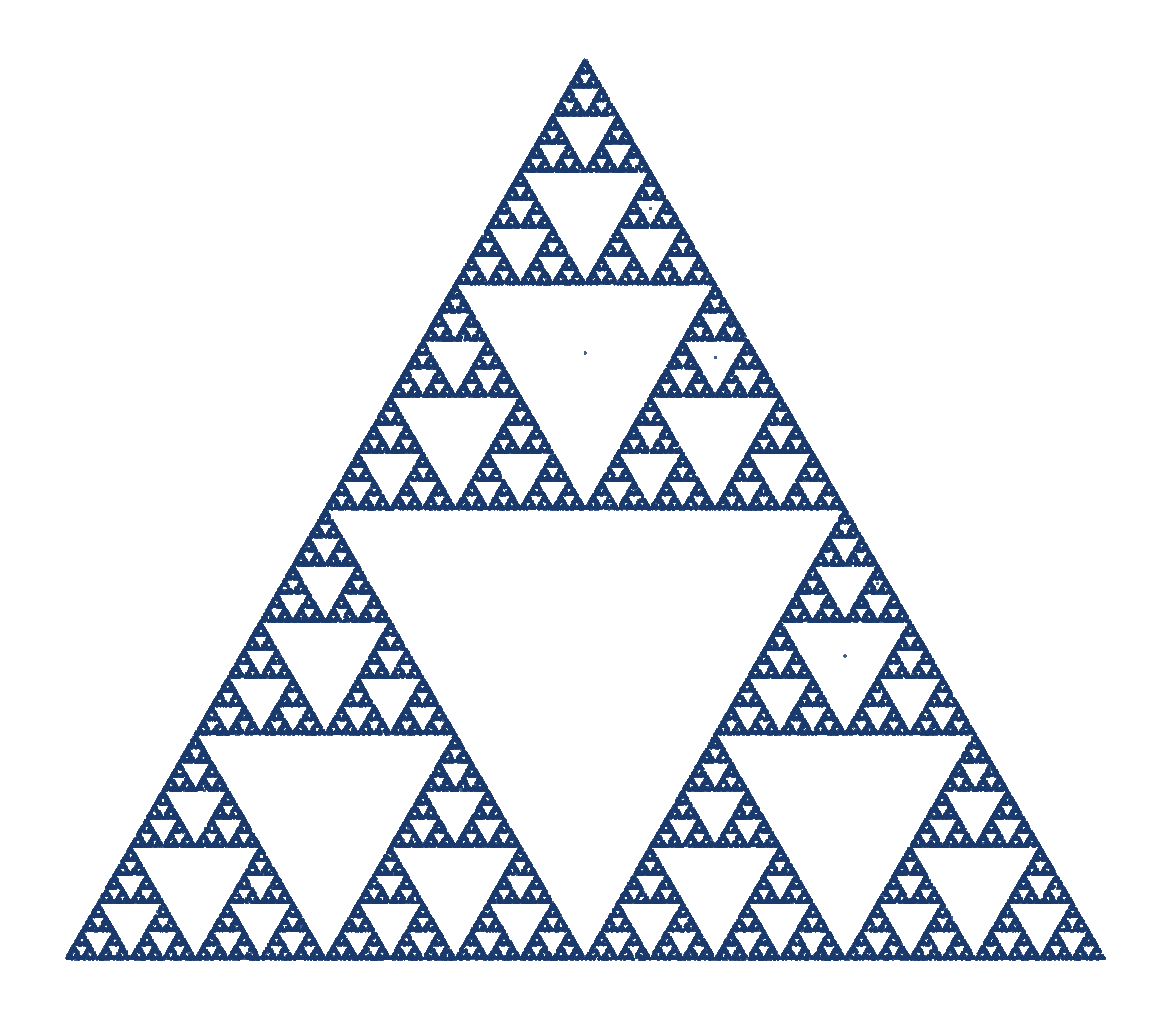
\includegraphics[height=4.6cm,keepaspectratio]{ch_fmh_sierpinski.pdf}\\[1pt]
{\scriptsize\textcolor{MediumGray}{\textit{Triunghiul Sierpinski generat prin chaos game.}}}
\end{column}
\end{columns}
\quantlet{SFM\_ch\_fmh\_fractals: sierpinski}{https://github.com/danpele/SFM/tree/main/Quantlets/SFM_ch_fmh}
\end{cminipage}
\end{frame}

\begin{frame}[shrink=15]{Coasta Britaniei: ,,Cât de lungă este coasta?''}
\begin{cminipage}{0.96\textwidth}
\begin{itemize}\setlength{\itemsep}{1pt}
    \item Mandelbrot (1967, \textit{Science}): lungimea măsurată depinde de \textbf{rigla} $\varepsilon$
    \item Legea de scalare: $L(\varepsilon)\propto\varepsilon^{1-D}$; pentru $D>1$, $L\to\infty$ când $\varepsilon\to 0$
    \item Britania: $D\approx 1{,}25$; Norvegia: $D\approx 1{,}52$ (mai zimțată, fiorduri)
    \item \textbf{Analogia financiară}: sub fBm/self-affine idealizat, $D\approx 2-H$ pentru graficul prețului (aproximație diagnostică pe date reale)
\end{itemize}
\centering
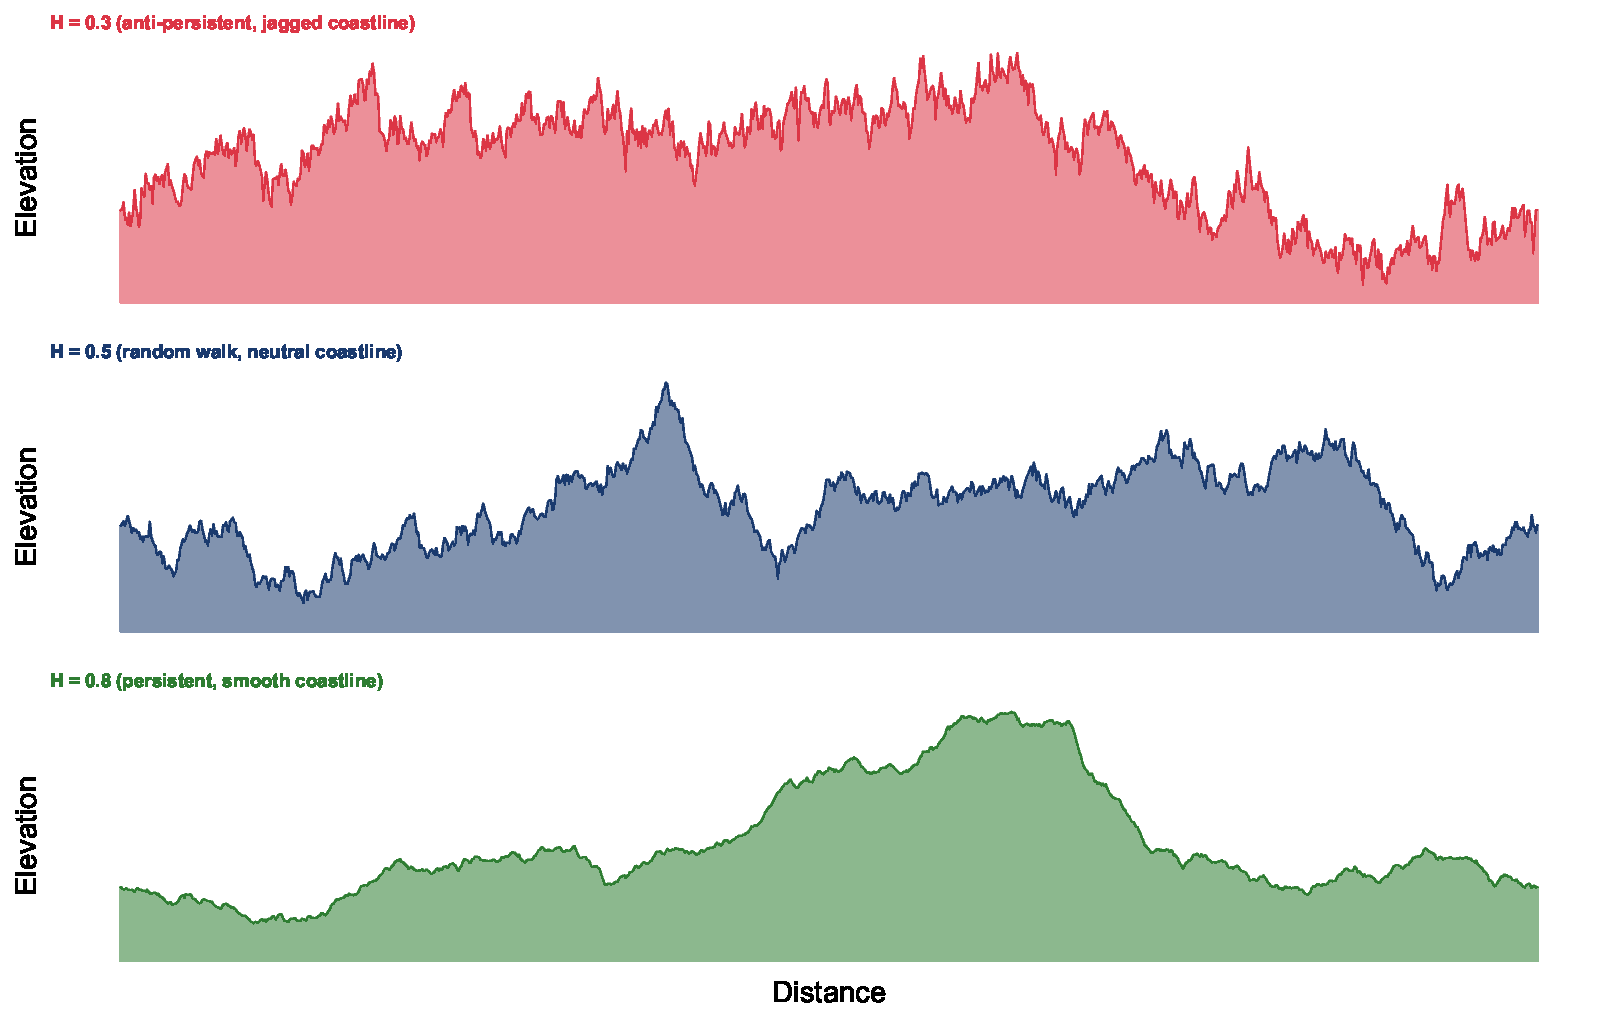
\includegraphics[width=0.92\linewidth,height=3.8cm,keepaspectratio]{ch_fmh_coastline.pdf}\\[1pt]
{\scriptsize\textcolor{MediumGray}{\textit{Țărmul real al Marii Britanii (Natural Earth 1:10m). Box-counting: $N(\varepsilon)$ crește când $\varepsilon$ scade --- pantă $\approx D$.}}}
\quantlet{SFM\_ch\_fmh\_fractals: coastline}{https://github.com/danpele/SFM/tree/main/Quantlets/SFM_ch_fmh}
\end{cminipage}
\end{frame}

\begin{frame}[shrink=15]{Box-counting: dimensiunea estimată din date}
\begin{cminipage}{0.95\textwidth}
\begin{defn}[Box-counting / Minkowski--Bouligand]
Fie $S\subset\R^d$ mărginită și $N(\varepsilon)$ numărul minim de cuburi de latură $\varepsilon$ care acoperă $S$:
\[
    D_{\text{box}}=\lim_{\varepsilon\to 0^+}\frac{\log N(\varepsilon)}{\log(1/\varepsilon)}.
\]
\end{defn}
\begin{columns}[T]
\begin{column}{0.55\textwidth}
\begin{itemize}\setlength{\itemsep}{0pt}
    \item \textbf{Estimare empirică}: regresie liniară a $\log N(\varepsilon)$ pe $\log(1/\varepsilon)$
    \item Pentru fractali ,,bine-comportați'': $D_{\text{box}}=\dim_H$ (Hausdorff)
    \item Pentru graficul prețului: $D_{\text{box}}=2-H$
    \item Cea mai folosită numeric (Hausdorff e dificil)
\end{itemize}
\end{column}
\begin{column}{0.42\textwidth}
\centering
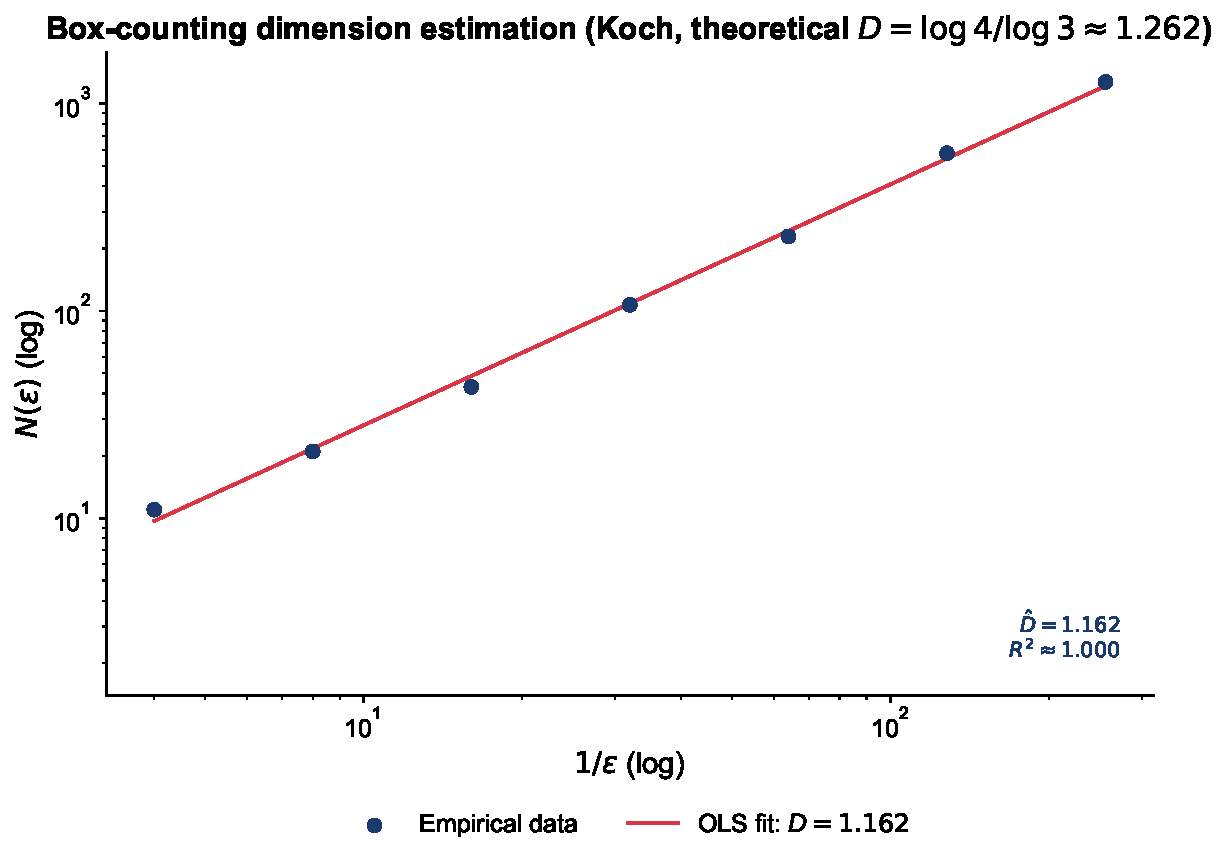
\includegraphics[width=\linewidth,height=4.4cm,keepaspectratio]{ch_fmh_boxcount_reg.pdf}\\[1pt]
{\scriptsize\textcolor{MediumGray}{\textit{Regresie log-log: pantă $\approx D$.}}}
\end{column}
\end{columns}
\quantlet{SFM\_ch\_fmh\_extra: boxcount}{https://github.com/danpele/SFM/tree/main/Quantlets/SFM_ch_fmh}
\end{cminipage}
\end{frame}

\begin{frame}[shrink=15]{Self-similarity statistică: prețul ca fractal}
\begin{cminipage}{0.95\textwidth}
\begin{defn}[Proces autosimilar (statistic)]
$\{X(t)\}_{t\geq 0}$ este \textbf{$H$-autosimilar} dacă, pentru orice $c>0$,
\[
    \{X(ct)\}_{t\geq 0}\stackrel{d}{=}\{c^{H} X(t)\}_{t\geq 0}.
\]
\end{defn}
\begin{columns}[T]
\begin{column}{0.50\textwidth}
\begin{block}{Exact (deterministic)}
\begin{itemize}\setlength{\itemsep}{0pt}
    \item $S=\bigcup_{i=1}^N f_i(S)$ cu $f_i$ contracții
    \item Cantor, Koch, Sierpinski, Mandelbrot
\end{itemize}
\end{block}
\end{column}
\begin{column}{0.46\textwidth}
\begin{alertblock}{Statistic (random)}
\begin{itemize}\setlength{\itemsep}{0pt}
    \item Distribuții finit-dim.\ invariante la scalare $c^H$
    \item fBm, fGn, cascade multiplicative
    \item Cazul piețelor: \textbf{auto-afinitate} (timp $\neq$ preț)
\end{itemize}
\end{alertblock}
\end{column}
\end{columns}
\vspace{0.1cm}
\begin{exampleblock}{Legea de scalare a volatilității}
\begin{itemize}\setlength{\itemsep}{0pt}
    \item Dacă $\ln P(t)$ este $H$-autosimilar: $\sigma(\Delta)=\sigma(1)\cdot \Delta^{H}$
    \item Sub EMH ($H=0{,}5$): regula clasică $\sqrt{\Delta}$
\end{itemize}
\end{exampleblock}
\end{cminipage}
\end{frame}

\begin{frame}[shrink=15]{Recap §II: 3 idei-cheie}
\begin{cminipage}{0.95\textwidth}
\begin{block}{De reținut}
\begin{enumerate}\setlength{\itemsep}{4pt}
    \item Dimensiunea fractală $D=\log N/\log(1/r)$ măsoară ,,cât de neregulat'' este un obiect autosimilar
    \item ,,Coasta Britaniei'': $L(\varepsilon)\propto\varepsilon^{1-D}$ --- introduce ideea de scalare dependentă de scală
    \item Pentru piețe: sub fBm/self-affine idealizat $D\approx 2-H$ (aproximație diagnostică, nu identitate universală); prețul este \textbf{fractal statistic}, nu doar mers aleator
\end{enumerate}
\end{block}
\begin{exampleblock}{Tranziție: \textit{,,acum trecem de la geometrie la estimare''}}
\begin{itemize}\setlength{\itemsep}{0pt}
    \item §III: cum estimăm operațional $\hat H$ din date $\Rightarrow$ R/S, Lo R/S, DFA, MFDFA
\end{itemize}
\end{exampleblock}
\end{cminipage}
\end{frame}

%#############################################################################
\section{Partea III: Estimare $\hat H$ [CORE]}
%#############################################################################

\begin{frame}[shrink=15]{Harold Hurst și problema Nilului}
\begin{cminipage}{0.95\textwidth}
\begin{columns}[T]
\begin{column}{0.55\textwidth}
\begin{itemize}\setlength{\itemsep}{1pt}
    \item \textbf{Context}
    \begin{itemize}\setlength{\itemsep}{0pt}
        \item Harold E.~Hurst (1880--1978), hidrolog britanic în Egipt
        \item Niveluri anuale ale Nilului (847--1284 d.Hr.)
        \item Problema: dimensionarea barajelor pe Nil
    \end{itemize}
    \item \textbf{Observație și estimare}
    \begin{itemize}\setlength{\itemsep}{0pt}
        \item Anii umezi tind să se grupeze; idem cei secetoși
        \item $\E[R(n)/S(n)]\propto n^H$; pentru Nil: $H\approx 0{,}73$
        \item ,,Efectul Joseph'' (Mandelbrot 1968) $\to$ ,,7 ani buni urmați de 7 răi''
    \end{itemize}
\end{itemize}
\end{column}
\begin{column}{0.42\textwidth}
\begin{block}{Mandelbrot \& Wallis (1969)}
\begin{itemize}\setlength{\itemsep}{0pt}
    \item Aplică R/S pe finanțe
    \item ,,Hurst este la geometria fractală ce este Bachelier la mersul aleator''
\end{itemize}
\end{block}
\end{column}
\end{columns}
\end{cminipage}
\end{frame}

\begin{frame}[shrink=15]{Definiția exponentului Hurst}
\begin{cminipage}{0.95\textwidth}
\begin{defn}[Exponentul Hurst]
$H\in(0,1)$ caracterizează structura de dependență pe termen lung. Sub R/S:
\[
    \E\!\left[\frac{R(n)}{S(n)}\right]\propto n^H,\quad n\to\infty.
\]
\end{defn}
\begin{itemize}\setlength{\itemsep}{0pt}
    \item $H=0{,}5$: mers aleator (fără memorie); consistent cu EMH
    \item $H>0{,}5$: persistent (trending); autocorelație pozitivă pe termen lung
    \item $H<0{,}5$: anti-persistent (mean-reverting); autocorelație negativă
\end{itemize}
\vspace{0.1cm}
\begin{exampleblock}{Relații centrale (sub fBm)}
\begin{itemize}\setlength{\itemsep}{0pt}
    \item Dimensiune fractală a graficului: $\boxed{D\approx 2-H}$ \quad (valabil pentru self-affine; pe date reale e diagnostic, nu identitate)
    \item Scalarea volatilității: $\sigma(\Delta)=\sigma(1)\Delta^H$
    \item Autocorelația incrementelor: $\rho(k)\sim H(2H-1)k^{2H-2}$
    \item Densitate spectrală a incrementelor (fGn): $S(\omega)\sim|\omega|^{1-2H}$ pentru $\omega\to 0$
\end{itemize}
\end{exampleblock}
\end{cminipage}
\end{frame}

\begin{frame}[shrink=15]{Cele 3 regimuri: tabel $H \to D$}
\begin{cminipage}{0.95\textwidth}
\begin{columns}[T]
\begin{column}{0.50\textwidth}
\renewcommand{\arraystretch}{1.2}
\centering
\begin{tabular}{ccl}
\toprule
$H$ & $D$ & \textbf{Interpretare} \\
\midrule
$0{,}1$ & $1{,}9$ & Foarte anti-persistent \\
$0{,}3$ & $1{,}7$ & Cu revenire la medie \\
$0{,}5$ & $1{,}5$ & Mers aleator \\
$0{,}7$ & $1{,}3$ & Persistent moderat \\
$0{,}9$ & $1{,}1$ & Foarte persistent \\
\bottomrule
\end{tabular}
\end{column}
\begin{column}{0.46\textwidth}
\begin{block}{Semnale (orientative, nu strategii directe)}
\begin{itemize}\setlength{\itemsep}{0pt}
    \item $H<0{,}5$: semnal compatibil cu strategii de tip contrar (cu revenire la medie)
    \item $H=0{,}5$: fără semnal liniar de tendință sau de inversare
    \item $H>0{,}5$: semnal compatibil cu strategii de urmărire a tendinței
    \item \textbf{Atenție}: niciuna dintre acestea nu garantează profit după costuri
\end{itemize}
\end{block}
\begin{alertblock}{Atenție}
\begin{itemize}\setlength{\itemsep}{0pt}
    \item Persistența $\neq$ ineficiență exploatabilă
    \item Costurile pot anula avantajul statistic
\end{itemize}
\end{alertblock}
\end{column}
\end{columns}
\end{cminipage}
\end{frame}

\begin{frame}[shrink=15]{Efectul Joseph și efectul Noah}
\begin{cminipage}{0.95\textwidth}
\begin{columns}[T]
\begin{column}{0.50\textwidth}
\begin{block}{Joseph (memorie lungă)}
\begin{itemize}\setlength{\itemsep}{0pt}
    \item ,,7 ani buni urmați de 7 răi'' (Geneza)
    \item Persistență, $H>0{,}5$
    \item Modelat de fBm și ARFIMA
\end{itemize}
\end{block}
\end{column}
\begin{column}{0.46\textwidth}
\begin{alertblock}{Noah (cozi grele)}
\begin{itemize}\setlength{\itemsep}{0pt}
    \item Potopul biblic --- evenimente catastrofale, discontinue
    \item Capturat de exponentul $\alpha$ Lévy ($\alpha<2$)
    \item Modelat de procese Lévy stabile (Cap.~2)
\end{itemize}
\end{alertblock}
\end{column}
\end{columns}
\vspace{0.2cm}
\begin{exampleblock}{Combinare}
\begin{itemize}\setlength{\itemsep}{0pt}
    \item \textbf{Mișcarea stabilă liniar-fracționară (LFSM, ,,Linear Fractional Stable Motion'')}: permite simultan memorie lungă (Joseph) și salturi (Noah)
    \item Generalizare a fBm cu inovații $\alpha$-stabile
    \item Cele două ,,boli'' ale piețelor financiare sunt acum modelate împreună
\end{itemize}
\end{exampleblock}
\end{cminipage}
\end{frame}

\begin{frame}[shrink=15]{Algoritmul scalării reescalate (R/S, \textit{Rescaled Range}; Hurst 1951)}
\begin{cminipage}{0.95\textwidth}
\begin{block}{Pași pentru o serie $\{x_1,\ldots,x_N\}$}
\begin{enumerate}\setlength{\itemsep}{1pt}
    \item Pentru $n\in\{n_1,\ldots,n_K\}$ (mărimi de bloc):
    \begin{itemize}\setlength{\itemsep}{0pt}
        \item Împarte seria în blocuri non-suprapuse de mărime $n$
        \item Pentru fiecare bloc: $Y_k=\sum_{i=1}^k(x_i-\bar x)$, $R=\max Y_k-\min Y_k$, $S=$ deviația standard
        \item $(R/S)_n=$ media pe blocuri
    \end{itemize}
    \item Regresie OLS: $\log(R/S)_n=\hat H\cdot\log n+c$
    \item Panta = $\hat H$ (exponentul Hurst)
\end{enumerate}
\end{block}
\begin{exampleblock}{Interpretare}
\begin{itemize}\setlength{\itemsep}{0pt}
    \item Sub $H_0$ (random walk): $\E[R(n)/S(n)]\propto n^{1/2}$
    \item Sub $H_1$ (memorie lungă): $\E[R(n)/S(n)]\propto n^H$, $H\neq 1/2$
\end{itemize}
\end{exampleblock}
\quantlet{SFM\_ch14\_fractal\_hurst}{https://github.com/danpele/SFM/tree/main/Quantlets/SFM_ch14}
\end{cminipage}
\end{frame}

\begin{frame}[shrink=15]{R/S exemplu pas-cu-pas pe serie de 8 puncte}
\begin{cminipage}{0.95\textwidth}
\begin{exampleblock}{Date}
\begin{itemize}\setlength{\itemsep}{0pt}
    \item Serie de 8 randamente: $x=\{0{,}5;\,-0{,}3;\,0{,}8;\,-0{,}2;\,0{,}6;\,-0{,}1;\,0{,}4;\,-0{,}7\}$
    \item Mărime bloc: $n=8$ (un singur bloc)
\end{itemize}
\end{exampleblock}
\begin{itemize}\setlength{\itemsep}{0pt}
    \item \textbf{Pasul 1}: media $\bar x=(0{,}5-0{,}3+0{,}8-0{,}2+0{,}6-0{,}1+0{,}4-0{,}7)/8=1{,}0/8=0{,}125$
    \item \textbf{Pasul 2}: cumulate $Y_k=\sum_{i=1}^k(x_i-\bar x)$
    \begin{itemize}\setlength{\itemsep}{0pt}
        \item $Y=\{0{,}375;\,-0{,}050;\,0{,}625;\,0{,}300;\,0{,}775;\,0{,}550;\,0{,}825;\,0\}$
    \end{itemize}
    \item \textbf{Pasul 3}: $R=\max Y-\min Y=0{,}825-(-0{,}050)=0{,}875$; $S\approx 0{,}490$
    \item \textbf{Pasul 4}: $R/S=0{,}875/0{,}490\approx \mathbf{1{,}786}$ pentru $n=8$
    \item \textbf{Pasul 5}: repetă pentru $n\in\{4,8,16,32,\ldots\}$ și fă regresie OLS pe $\log(R/S)_n$ vs $\log n$
\end{itemize}
\end{cminipage}
\end{frame}

\begin{frame}[shrink=25]{Mini-exercițiu B: $R/S$ pe 4 puncte}
\begin{cminipage}{0.95\textwidth}
\begin{block}{Sarcină}
\begin{itemize}\setlength{\itemsep}{0pt}
    \item Fie $x=\{1;\,3;\,2;\,4\}$. Calculați $R/S$ pentru $n=4$.
\end{itemize}
\end{block}
\begin{block}{Pași}
\begin{enumerate}\setlength{\itemsep}{0pt}
    \item Calculați media $\bar x$
    \item Construiți seria cumulativă a deviațiilor $Y_k=\sum_{i\leq k}(x_i-\bar x)$
    \item Calculați amplitudinea $R=\max Y_k-\min Y_k$ și abaterea standard $S$
    \item Raportul $R/S$
\end{enumerate}
\end{block}
\begin{exampleblock}{Răspuns}
\begin{itemize}\setlength{\itemsep}{0pt}
    \item $\bar x=10/4=2{,}5$; deviații $\{-1{,}5;\,0{,}5;\,-0{,}5;\,1{,}5\}$; $Y=\{-1{,}5;\,-1{,}0;\,-1{,}5;\,0\}$
    \item $R=0-(-1{,}5)=1{,}5$; $S=\sqrt{1{,}25}\approx 1{,}118$
    \item $R/S\approx \mathbf{1{,}342}$
\end{itemize}
\end{exampleblock}
\begin{alertblock}{Interpretare}
\begin{itemize}\setlength{\itemsep}{0pt}
    \item Pe un singur $n$ \textbf{nu} putem estima $H$: avem nevoie de scalare pe mai multe $n$ și regresie log-log a $\overline{R/S}$ pe $\log n$
    \item Acest exercițiu testează doar mecanica formulei R/S, nu identificarea memoriei lungi
\end{itemize}
\end{alertblock}
\end{cminipage}
\end{frame}

\begin{frame}[shrink=15]{R/S: cum citim regresia OLS finală}
\begin{cminipage}{0.95\textwidth}
\begin{block}{Regresia $\log(R/S)_n=\hat H\cdot\log n+c$}
\begin{itemize}\setlength{\itemsep}{0pt}
    \item Axa $x$: $\log n$ pentru fiecare $n\in\{n_1,\ldots,n_K\}$
    \item Axa $y$: $\log\overline{(R/S)_n}$ (medie pe blocuri)
    \item Panta = $\hat H$; intercept = $c$ (informație despre constanta de proporționalitate)
\end{itemize}
\end{block}
\begin{exampleblock}{Sfaturi practice}
\begin{itemize}\setlength{\itemsep}{0pt}
    \item Folosește mărimi de bloc \textbf{geometric distribuite}: $n=2^k$ sau $n=10^{0{,}25k}$
    \item Limită jos: $n_{\min}\geq 10$ (eșantion suficient pentru $S$)
    \item Limită sus: $n_{\max}\leq N/4$ (suficiente blocuri pentru medie)
    \item Verifică liniaritatea: dacă există \textbf{crossover}, raportează 2 regimuri ($\hat H_1,\hat H_2$)
    \item Eroare standard: bootstrap pe blocuri
\end{itemize}
\end{exampleblock}
\end{cminipage}
\end{frame}

\begin{frame}[shrink=15]{R/S modificat (Lo, 1991): corecție pentru dependența pe termen scurt}
\begin{cminipage}{0.95\textwidth}
\begin{alertblock}{Critica Lo (1991)}
\begin{itemize}\setlength{\itemsep}{0pt}
    \item R/S clasică \textbf{confundă memoria pe termen lung cu cea pe termen scurt} (autocorelații pe decalaje mici)
    \item Lo propune o \textbf{corecție pentru dependența pe termen scurt}
    \item Corecția vizează autocorelația pe termen scurt, NU GARCH
\end{itemize}
\end{alertblock}
\begin{block}{Statistica modificată}
\[
    Q_n=\frac{R(n)}{\sigma_n(q)},\quad
    \sigma_n^2(q)=\hat\gamma_0+2\sum_{j=1}^{q}w_j(q)\hat\gamma_j,\quad w_j=1-\tfrac{j}{q+1}
\]
cu $\hat\gamma_j$ autocovarianța la decalajul $j$ și $w_j$ ponderi Bartlett (Newey--West).
\end{block}
\begin{itemize}\setlength{\itemsep}{0pt}
    \item Sub $H_0:H=1/2$: $Q_n/\sqrt n \xrightarrow{d} V$ (Lo 1991, Tabel I)
    \item Test la $\alpha=5\%$: \textbf{respinge} dacă $Q_n/\sqrt n\notin[0{,}809;\,1{,}862]$
\end{itemize}
\end{cminipage}
\end{frame}

\begin{frame}[shrink=15]{Analiza fluctuațiilor cu eliminarea trendului (DFA, \textit{Detrended Fluctuation Analysis}) --- alternativă robustă la trenduri}
\begin{cminipage}{0.95\textwidth}
\begin{block}{Algoritm DFA (Peng et al., 1994)}
\begin{enumerate}\setlength{\itemsep}{1pt}
    \item Calculează profilul $Y_k=\sum_{i=1}^k(x_i-\bar{x})$
    \item Împarte $\{Y_k\}$ în segmente non-suprapuse de mărime $n$
    \item În fiecare segment, ajustează polinom de ordin $m$ (DFA-$m$)
    \item Funcția de fluctuație: $F(n)=\sqrt{\frac{1}{N}\sum(Y_k-\hat{Y}_k^{(m)})^2}$
    \item Regresie: $\log F(n)\sim H\log n$
\end{enumerate}
\end{block}
\begin{itemize}\setlength{\itemsep}{0pt}
    \item Avantaj față de R/S: \textbf{robust la trenduri polinomiale} de grad $\leq m$
    \item Standard: \textbf{DFA-1} pentru randamente; DFA-2/3 pentru prețuri non-staționare
    \item DFA aplicat pe \textbf{randamente} (fGn): exponent $\alpha=H$ (Hurst-ul fBm-ului asociat); pe \textbf{prețuri/fBm}: $\alpha=H+1$ (integrare suplimentară)
\end{itemize}
\end{cminipage}
\end{frame}

\begin{frame}[shrink=15]{Limitări R/S și DFA: capcane practice}
\begin{cminipage}{0.95\textwidth}
\begin{alertblock}{Capcane}
\begin{itemize}\setlength{\itemsep}{2pt}
    \item Eșantioane scurte $\Rightarrow$ $\hat{H}$ instabil; interval de încredere larg
    \item \textbf{Rupturile structurale} și \textbf{schimbările de regim} pot da $\hat{H}>0{,}5$ \textbf{spurios} (Granger \& Ding 1996; Diebold \& Inoue 2001; Mikosch \& Stărică 2004)
    \item GARCH și aglomerarea volatilității pot perturba R/S clasic
    \item \textbf{Zgomotul de microstructură} la frecvențe înalte
    \item Trenduri nestaționare $\Rightarrow$ folosiți DFA-2/3
    \item Alegerea ferestrei $[n_{\min},n_{\max}]$ afectează panta
\end{itemize}
\end{alertblock}
\begin{exampleblock}{Diagnostic standard}
\begin{itemize}\setlength{\itemsep}{0pt}
    \item Raportați întotdeauna: (a) $\hat H$ pe sub-eșantioane (estimare mobilă); (b) puncte de ruptură Bai--Perron; (c) DFA pe reziduuri după eliminarea trendului
\end{itemize}
\end{exampleblock}
\end{cminipage}
\end{frame}

\begin{frame}[shrink=15]{Recap §III: 3 idei-cheie}
\begin{cminipage}{0.95\textwidth}
\begin{block}{De reținut}
\begin{enumerate}\setlength{\itemsep}{4pt}
    \item R/S clasic: pași simpli, dar sensibil la dependența pe termen scurt; \textbf{Lo (1991)} corectează prin Newey--West
    \item DFA = standardul modern (robust la trenduri polinomiale); MFDFA (\textit{Multifractal DFA}) pentru spectrul multifractal
    \item \textbf{Combinație recomandată}: DFA-1 + Variance Ratio + Lo R/S + (opțional) MFDFA; raportați limitările și intervalul de încredere
\end{enumerate}
\end{block}
\begin{exampleblock}{Tranziție: \textit{,,acum trecem de la estimator la interpretare pe date reale''}}
\begin{itemize}\setlength{\itemsep}{0pt}
    \item §IV: aplicăm metodele pe date reale --- SPY, BTC, BET, FX
\end{itemize}
\end{exampleblock}
\end{cminipage}
\end{frame}

%#############################################################################
\section{Partea IV: Hurst aplicat (SPY, BTC, BET) [CORE]}
%#############################################################################

\begin{frame}[shrink=15]{Quantlet SFM\_ch14\_fractal\_hurst --- A: estimare statică}
\begin{cminipage}{0.96\textwidth}
\centering
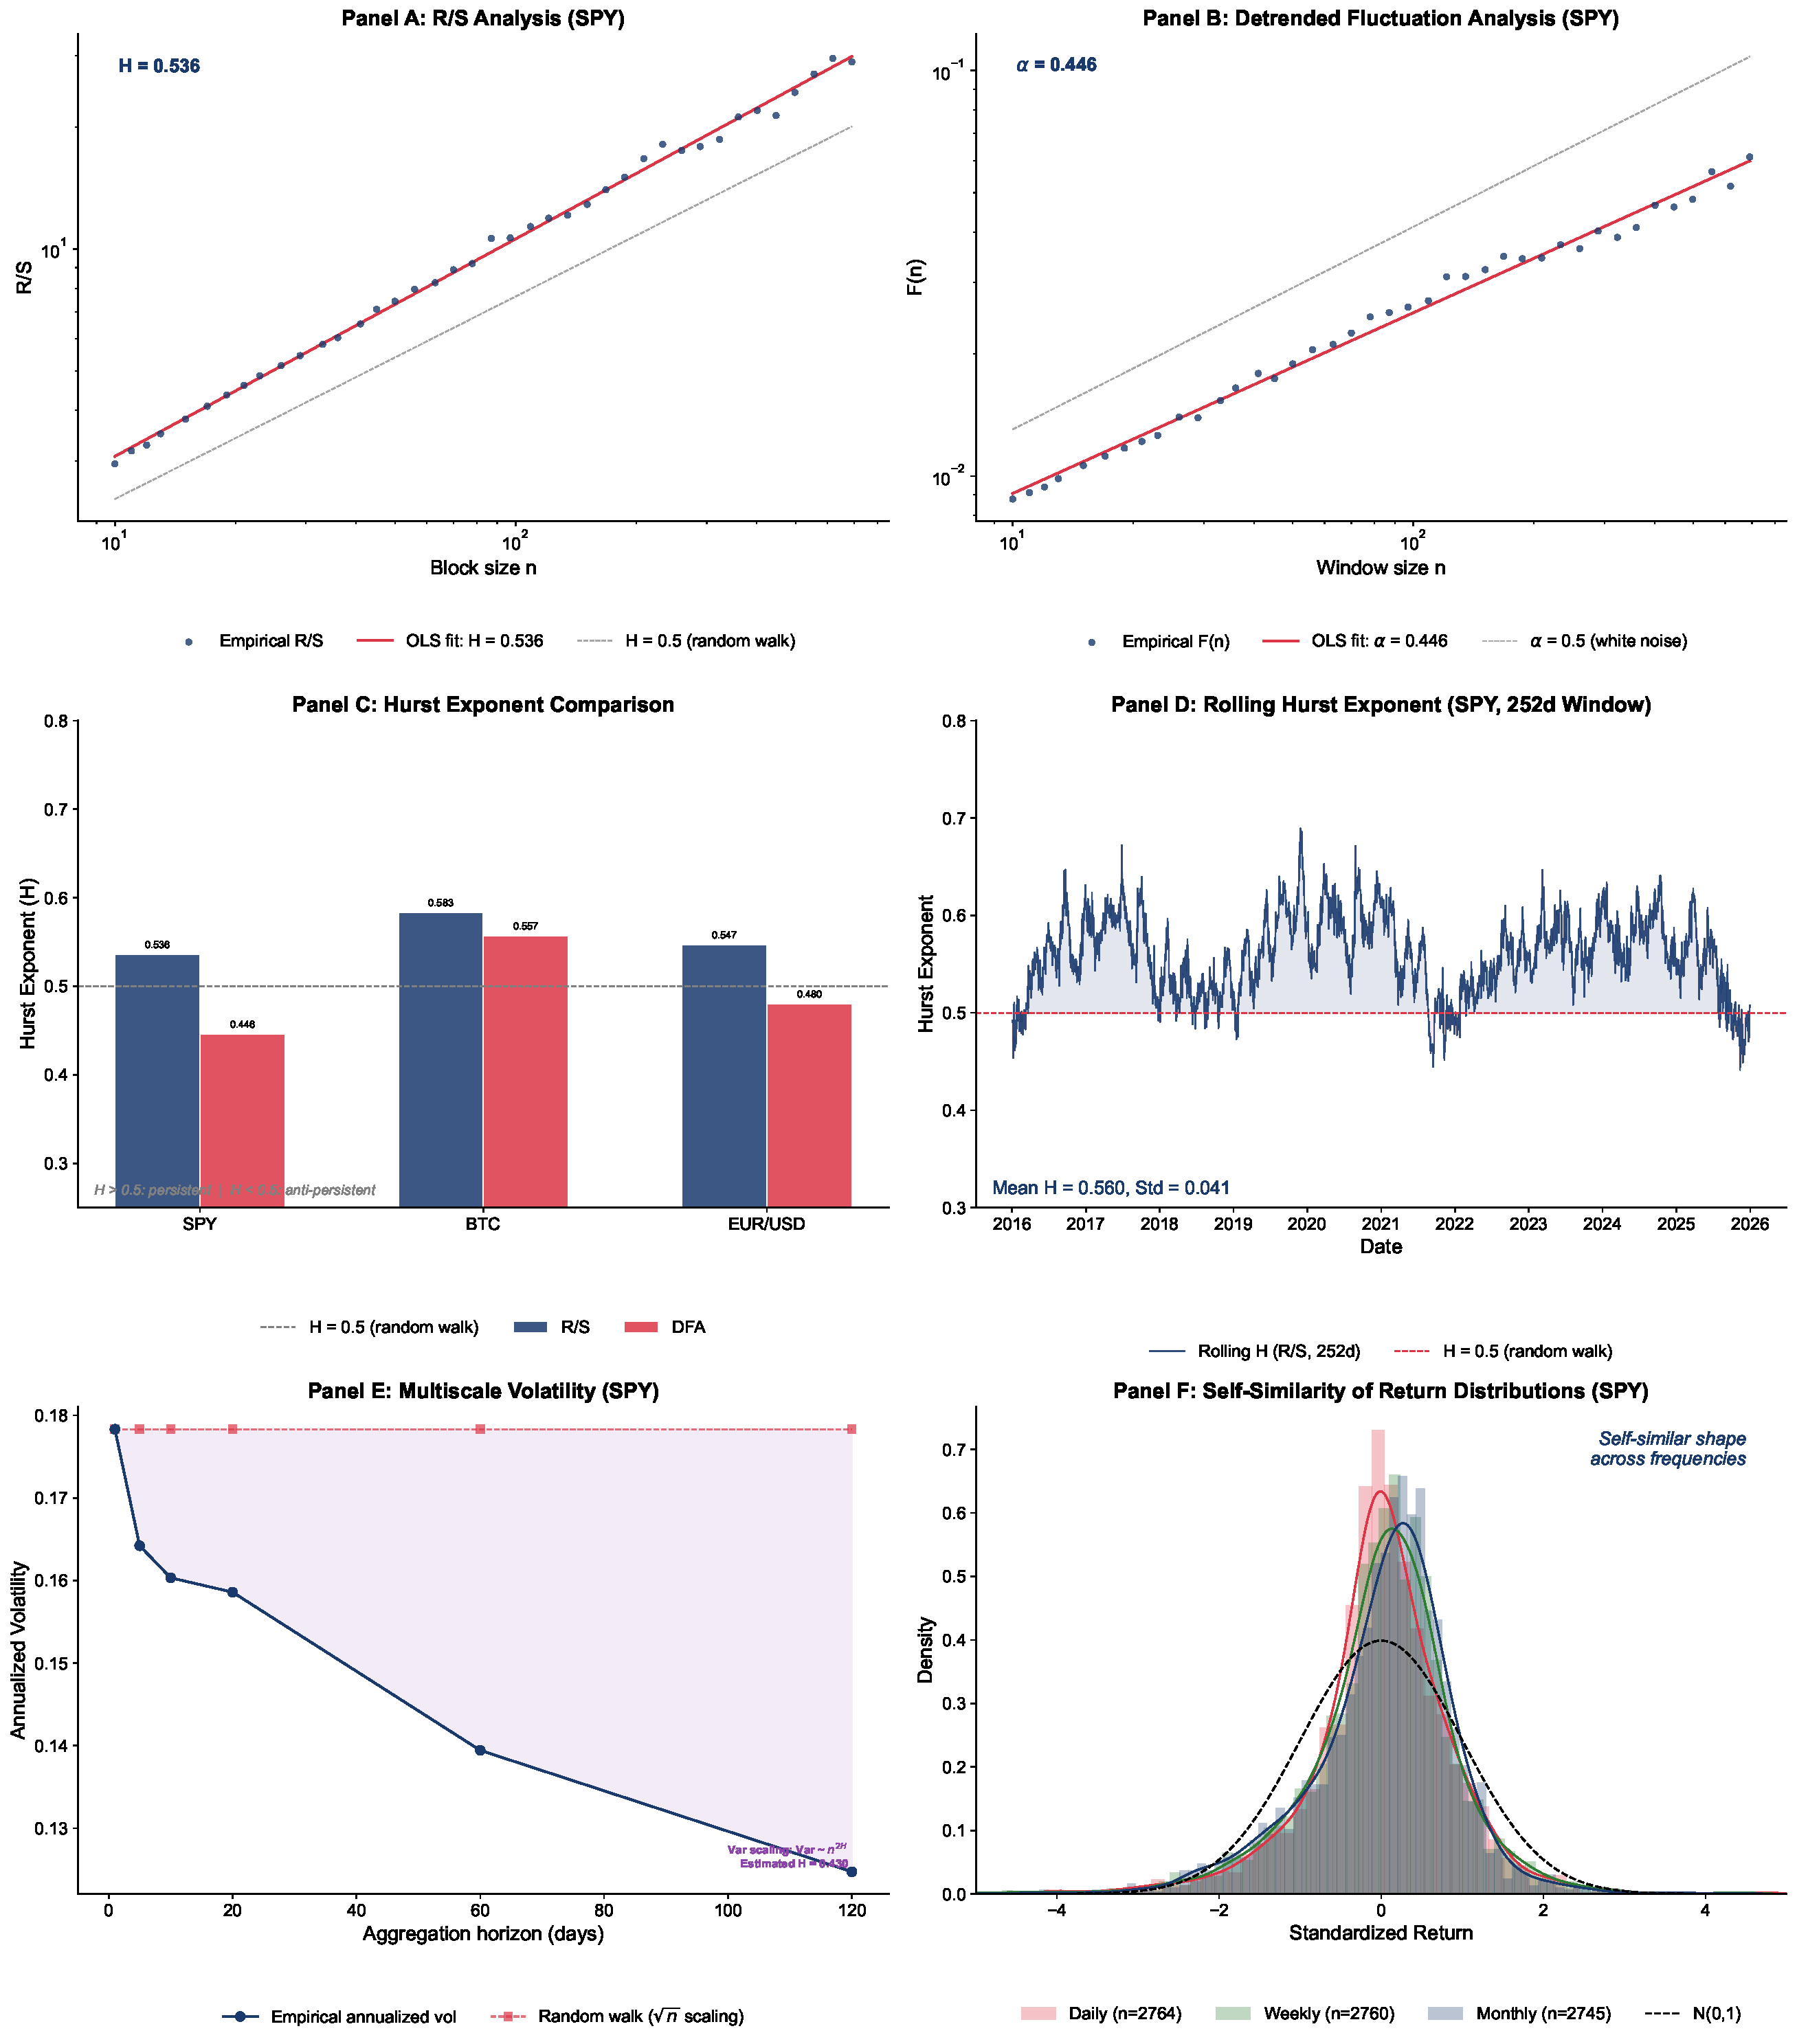
\includegraphics[width=0.86\linewidth,height=6.0cm,keepaspectratio]{ch14_fractal_hurst.pdf}\\[2pt]
{\footnotesize\textcolor{MediumGray}{\textit{Panourile A--C: scalarea R/S pe SPY (panta $\approx H$); DFA pe SPY; comparație $\hat H$ pe SPY, BTC, EUR/USD.}}}
\end{cminipage}
\quantlet{SFM\_ch14\_fractal\_hurst}{https://github.com/danpele/SFM/tree/main/Quantlets/SFM_ch14}
\end{frame}

\begin{frame}[shrink=15]{Quantlet SFM\_ch14\_fractal\_hurst --- B: dinamică și distribuție}
\begin{cminipage}{0.96\textwidth}
\centering
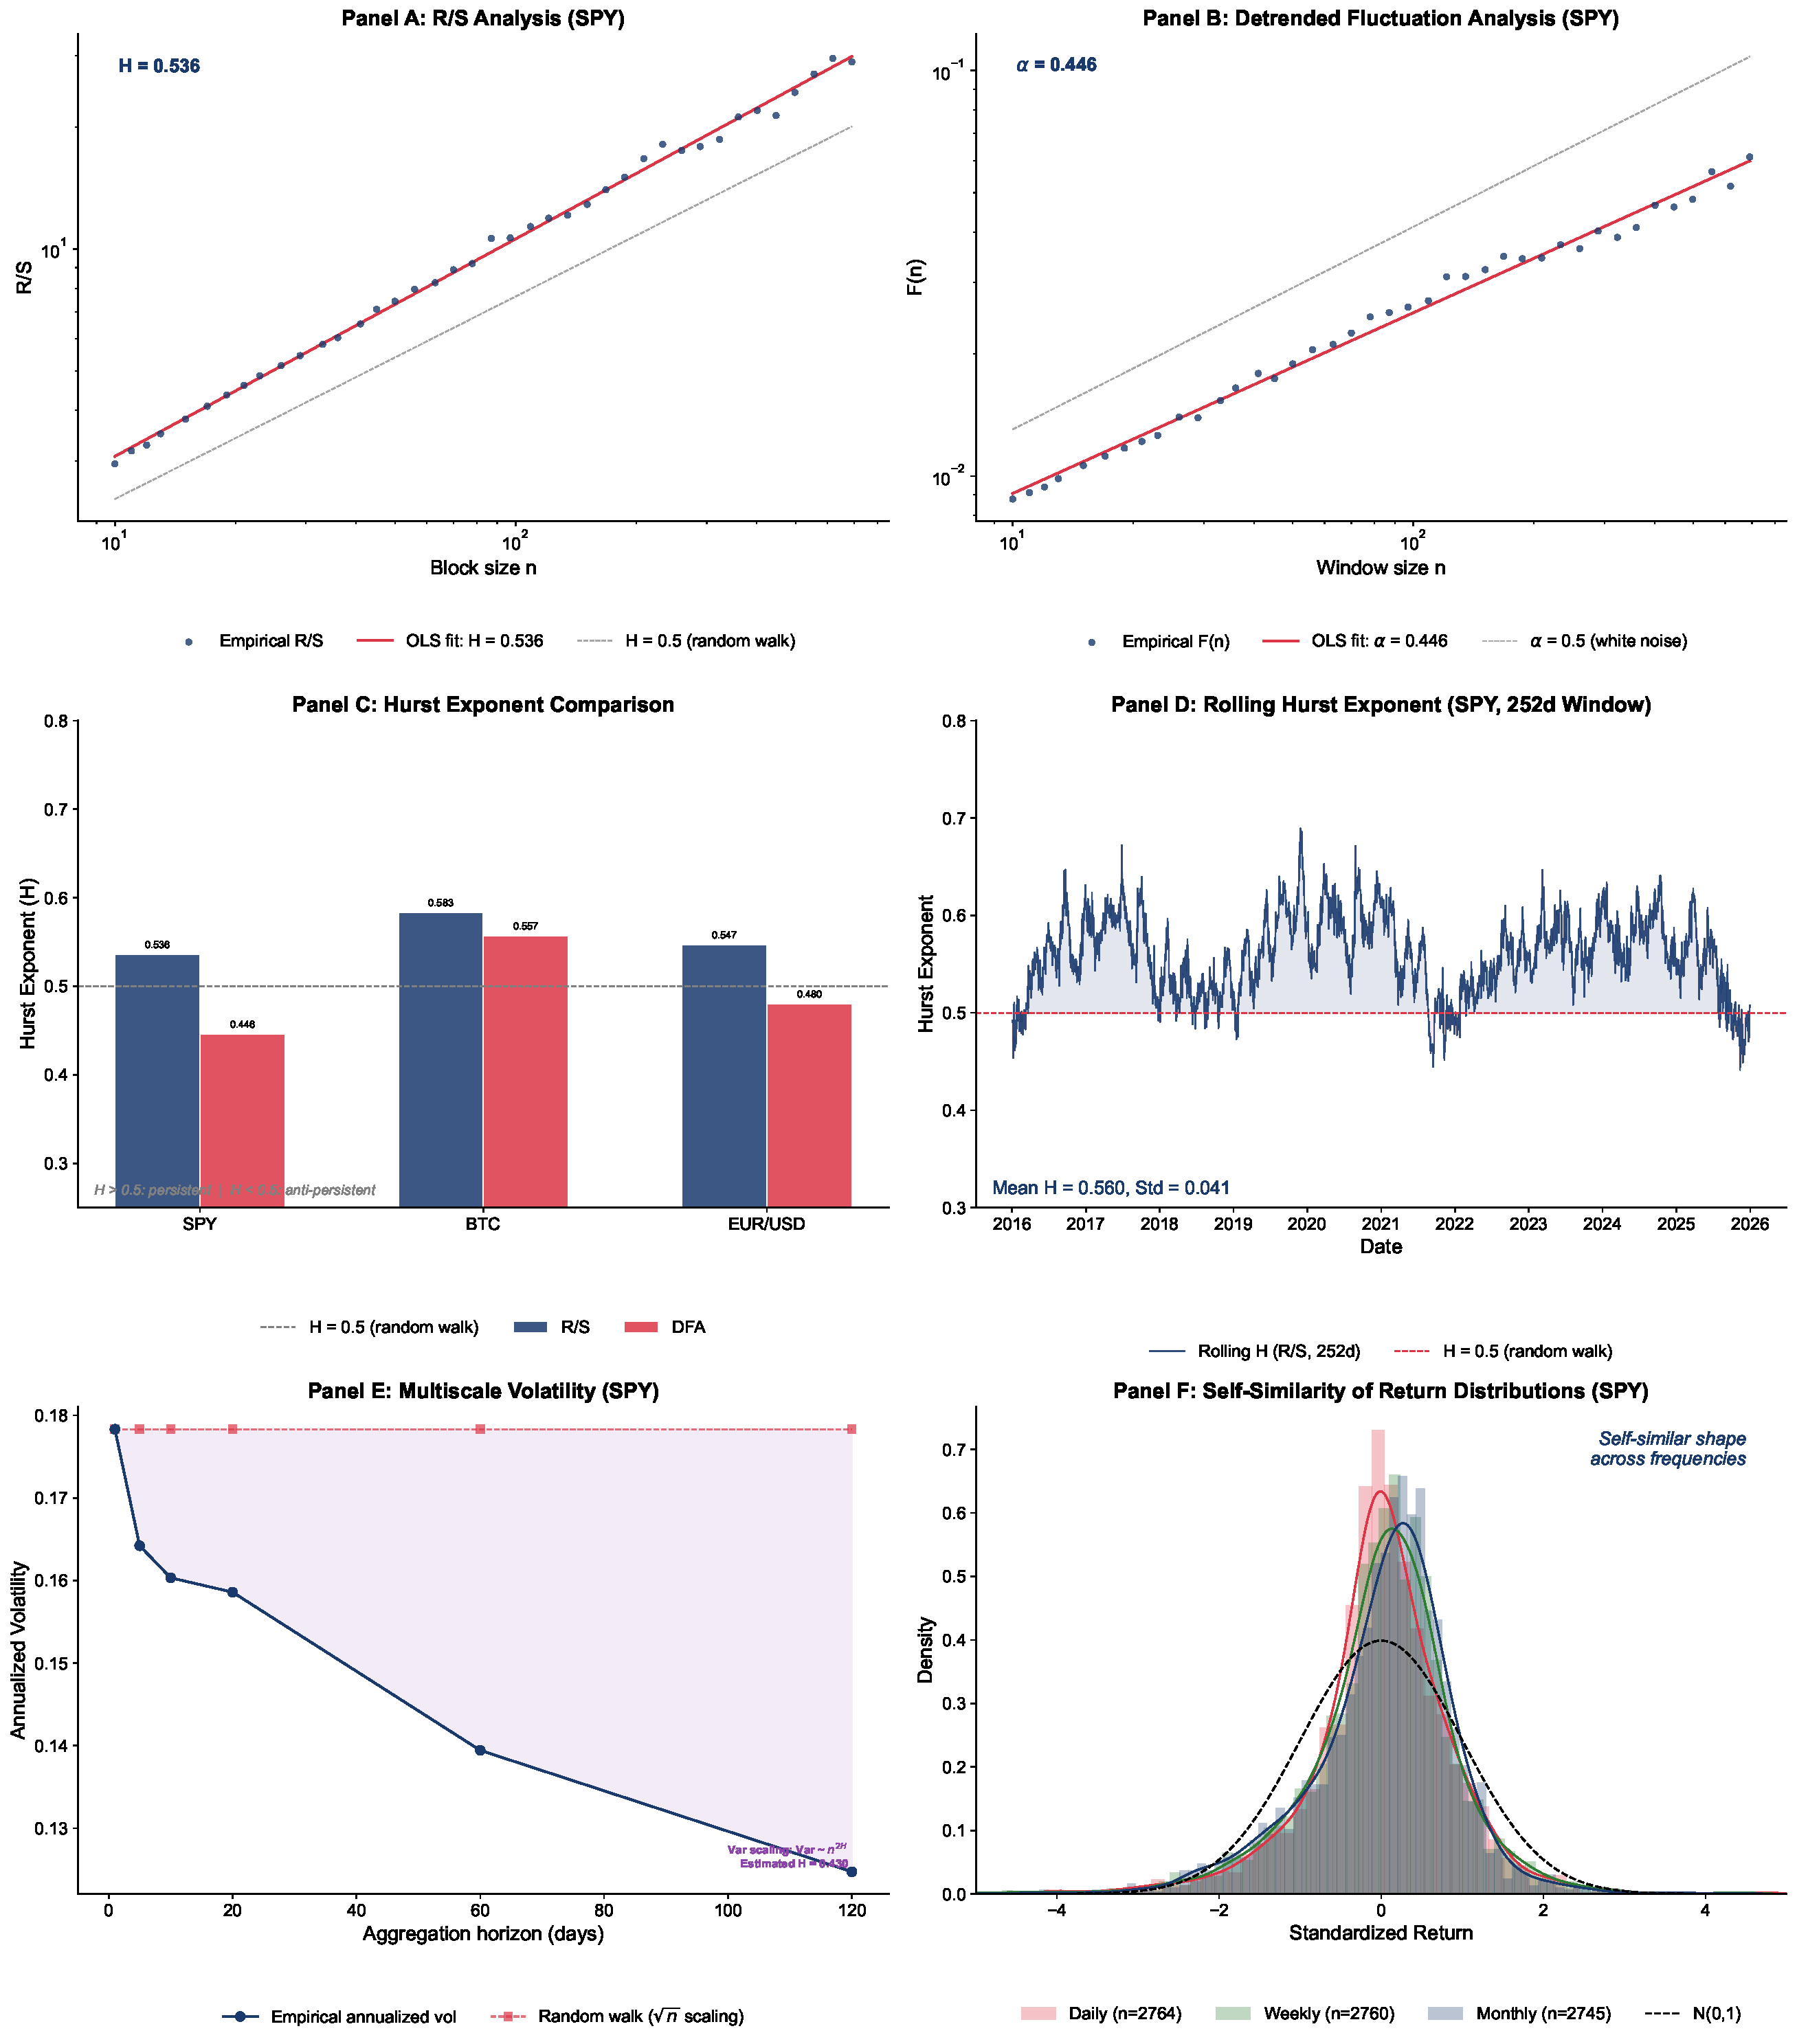
\includegraphics[width=0.86\linewidth,height=6.0cm,keepaspectratio]{ch14_fractal_hurst.pdf}\\[2pt]
{\footnotesize\textcolor{MediumGray}{\textit{Panourile D--F: $\hat H_t$ pe fereastră mobilă (252 zile); scalarea volatilității multi-orizont; autosimilaritate distribuțională.}}}
\end{cminipage}
\quantlet{SFM\_ch14\_fractal\_hurst}{https://github.com/danpele/SFM/tree/main/Quantlets/SFM_ch14}
\end{frame}

\begin{frame}[shrink=15]{Estimări $\hat H$ pe clase de active}
\begin{cminipage}{0.95\textwidth}
\renewcommand{\arraystretch}{1.2}
\centering
\small
\begin{tabular}{lll}
\toprule
\textbf{Clasă / piață} & \textbf{$\hat{H}$ tipic} & \textbf{Metodă} \\
\midrule
S\&P~500 (SPY) & $0{,}55$--$0{,}62$ & R/S, DFA \\
FTSE~100 & $0{,}53$--$0{,}60$ & DFA \\
DAX~30 & $0{,}54$--$0{,}61$ & R/S, DFA \\
Nikkei~225 & $0{,}52$--$0{,}59$ & DFA \\
\textbf{BET (BVB)} & $\mathbf{0{,}60}$--$\mathbf{0{,}72}$ & R/S, DFA \\
Bitcoin (BTC) & $0{,}50$--$0{,}75$ & DFA, wavelet \\
EUR/USD & $0{,}50$--$0{,}55$ & R/S, DFA \\
Aur (XAU) & $0{,}52$--$0{,}58$ & DFA \\
\bottomrule
\end{tabular}
\vspace{0.15cm}
\begin{itemize}\setlength{\itemsep}{0pt}
    \item Piețe \textbf{dezvoltate}: $\hat{H}$ aproape de $0{,}5$
    \item Piețe \textbf{emergente} (BVB): $\hat{H}\in[0{,}6;\,0{,}7]$ $\Rightarrow$ memorie lungă, eficiență redusă
    \item Forex (cel mai lichid): $\hat{H}$ aproape de EMH
    \item Bitcoin: tranziție clasică ineficient $\to$ cvasi-eficient pe măsură ce maturizează
\end{itemize}
\end{cminipage}
\end{frame}

\begin{frame}[shrink=15]{Capcane de interpretare: $H>0{,}5$ NU $\Rightarrow$ profit garantat}
\begin{cminipage}{0.95\textwidth}
\begin{alertblock}{$H>0{,}5$ NU implică ineficiență exploatabilă}
\begin{itemize}\setlength{\itemsep}{2pt}
    \item Persistența nu este sinonimă cu \textbf{ineficiență exploatabilă}
    \item Costurile de tranzacționare pot anula avantajul statistic
    \item $\hat H$ este \textbf{instabil} pe sub-eșantioane (regimuri, rupturi structurale)
    \item Test primar pentru ineficiență: \textbf{Hurst/DFA/MFDFA + stabilitate pe regimuri}
\end{itemize}
\end{alertblock}
\begin{exampleblock}{Recomandare diagnostic}
\begin{itemize}\setlength{\itemsep}{0pt}
    \item Înainte de a interpreta $\hat H>0{,}5$ ca semnal de ineficiență, raportați:
    \begin{itemize}\setlength{\itemsep}{0pt}
        \item (i) interval de încredere bootstrap pentru $\hat H$
        \item (ii) $\hat H$ pe sub-perioade (fereastră mobilă de 252 zile)
        \item (iii) test Bai--Perron pentru puncte de ruptură
        \item (iv) testare retrospectivă cu costuri a unei strategii de tip ,,urmărirea tendinței''
    \end{itemize}
\end{itemize}
\end{exampleblock}
\end{cminipage}
\end{frame}

\begin{frame}[shrink=15]{Hurst pe fereastră mobilă pentru S\&P 500: eficiență dinamică}
\begin{cminipage}{0.95\textwidth}
\begin{columns}[T]
\begin{column}{0.55\textwidth}
\centering
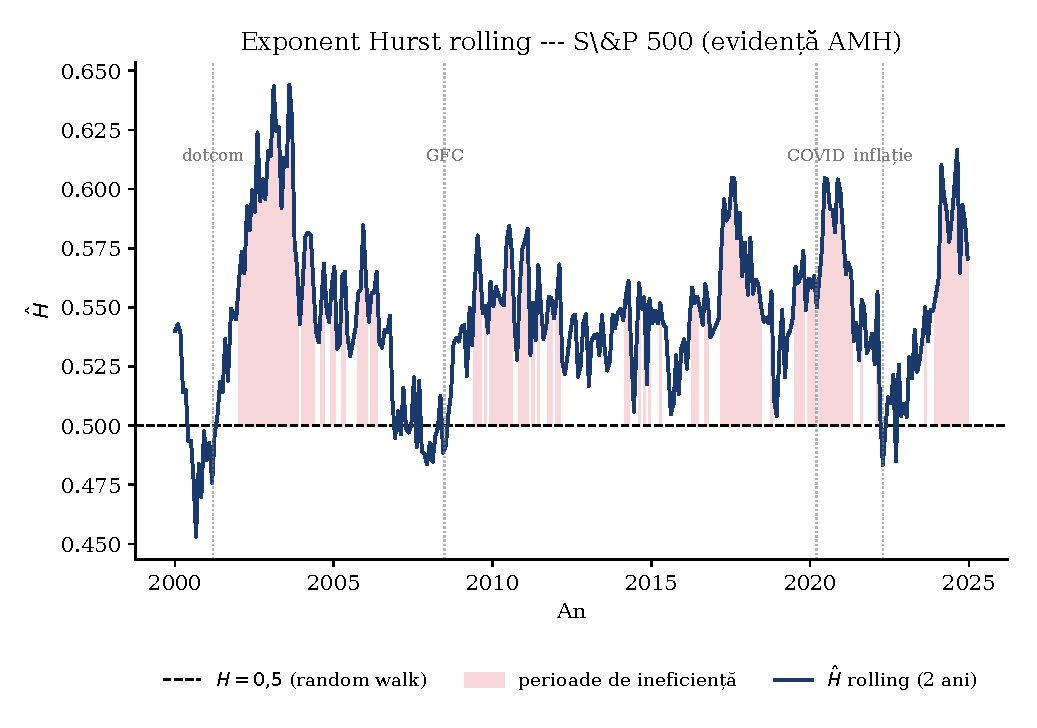
\includegraphics[width=\linewidth,height=4.6cm,keepaspectratio]{sfm_ch4_rolling_hurst.pdf}\\[2pt]
{\scriptsize\textcolor{MediumGray}{\textit{$\hat H_t$ pe fereastră mobilă de 252 zile, S\&P 500, 2000--2024.}}}
\end{column}
\begin{column}{0.42\textwidth}
\begin{block}{Observații}
\begin{itemize}\setlength{\itemsep}{0pt}
    \item $\hat H_t$ oscilează în jurul valorii $0{,}55$ în regim normal
    \item \textbf{Scăderi bruște spre/sub $0{,}5$}: 2008, COVID-2020
    \item Creșteri spre $0{,}65$: piețe cu tendință puternică (2017, 2021)
\end{itemize}
\end{block}
\begin{alertblock}{Consistent cu AMH (\textit{Adaptive Markets Hypothesis}; Lo 2004)}
\begin{itemize}\setlength{\itemsep}{0pt}
    \item Eficiența pieței variază în timp
    \item EMH = caz special (eficiență constantă)
\end{itemize}
\end{alertblock}
\end{column}
\end{columns}
\quantlet{SFM\_ch4\_rolling\_hurst}{https://github.com/danpele/SFM/tree/main/Quantlets/Ch_04/SFM_ch4_rolling_hurst}
\end{cminipage}
\end{frame}

\begin{frame}[shrink=25]{Mini-exercițiu C: interpretarea unui $\hat H_t$ pe fereastră mobilă}
\begin{cminipage}{0.95\textwidth}
\begin{block}{Sarcină}
\begin{itemize}\setlength{\itemsep}{0pt}
    \item Pe S\&P~500, $\hat H_t$ trece brusc de la $0{,}55$ la $0{,}48$ în trei luni
    \item Diagnosticați ce se întâmplă cu structura pieței și formulați o recomandare către un responsabil de risc
\end{itemize}
\end{block}
\begin{block}{Pași}
\begin{enumerate}\setlength{\itemsep}{0pt}
    \item Verificați robustețea: ferestre alternative, sub-eșantioane, DFA pe lângă R/S
    \item Identificați regimul: $H<0{,}5\Rightarrow$ anti-persistență
    \item Mapati semnalul în limbaj FMH: diversitate de orizonturi, lichiditate
\end{enumerate}
\end{block}
\begin{exampleblock}{Răspuns}
\begin{itemize}\setlength{\itemsep}{0pt}
    \item Diagnostic FMH: \textbf{colaps al orizonturilor} (investitori pe termen lung părăsesc piața; domină tranzacționarea pe termen scurt)
    \item $H<0{,}5$ $\Rightarrow$ anti-persistență (reversie/inversare frecventă)
    \item Recomandări: reducerea expunerii, test de stres VaR cu $T^H$, diversificare către active cu $H$ stabil
\end{itemize}
\end{exampleblock}
\begin{alertblock}{Interpretare}
\begin{itemize}\setlength{\itemsep}{0pt}
    \item Semnalul trebuie validat (sub-eșantioane, costuri, regim de lichiditate); $\hat H_t$ \emph{nu} este o regulă de decizie automată
\end{itemize}
\end{alertblock}
\end{cminipage}
\end{frame}

\begin{frame}[shrink=15]{Bitcoin: evoluția eficienței}
\begin{cminipage}{0.95\textwidth}
\begin{columns}[T]
\begin{column}{0.55\textwidth}
\begin{itemize}\setlength{\itemsep}{1pt}
    \item \textbf{Cronologia lui $\hat H$ pe BTC}
    \begin{itemize}\setlength{\itemsep}{0pt}
        \item 2010--2014 (etapa incipientă): $\hat H_{\text{BTC}}\approx 0{,}70$--$0{,}80$
        \item 2015--2018 (maturizare): $\approx 0{,}55$--$0{,}65$ (contracte futures CME, dec.\ 2017)
        \item 2019--prezent: $\approx 0{,}50$--$0{,}55$ (ETF spot, ian.\ 2024)
    \end{itemize}
    \item \textbf{Interpretare}
    \begin{itemize}\setlength{\itemsep}{0pt}
        \item Tranziție clasică: piață ineficientă $\to$ cvasi-eficientă, similară cu piețele FX
    \end{itemize}
\end{itemize}
\end{column}
\begin{column}{0.42\textwidth}
\centering
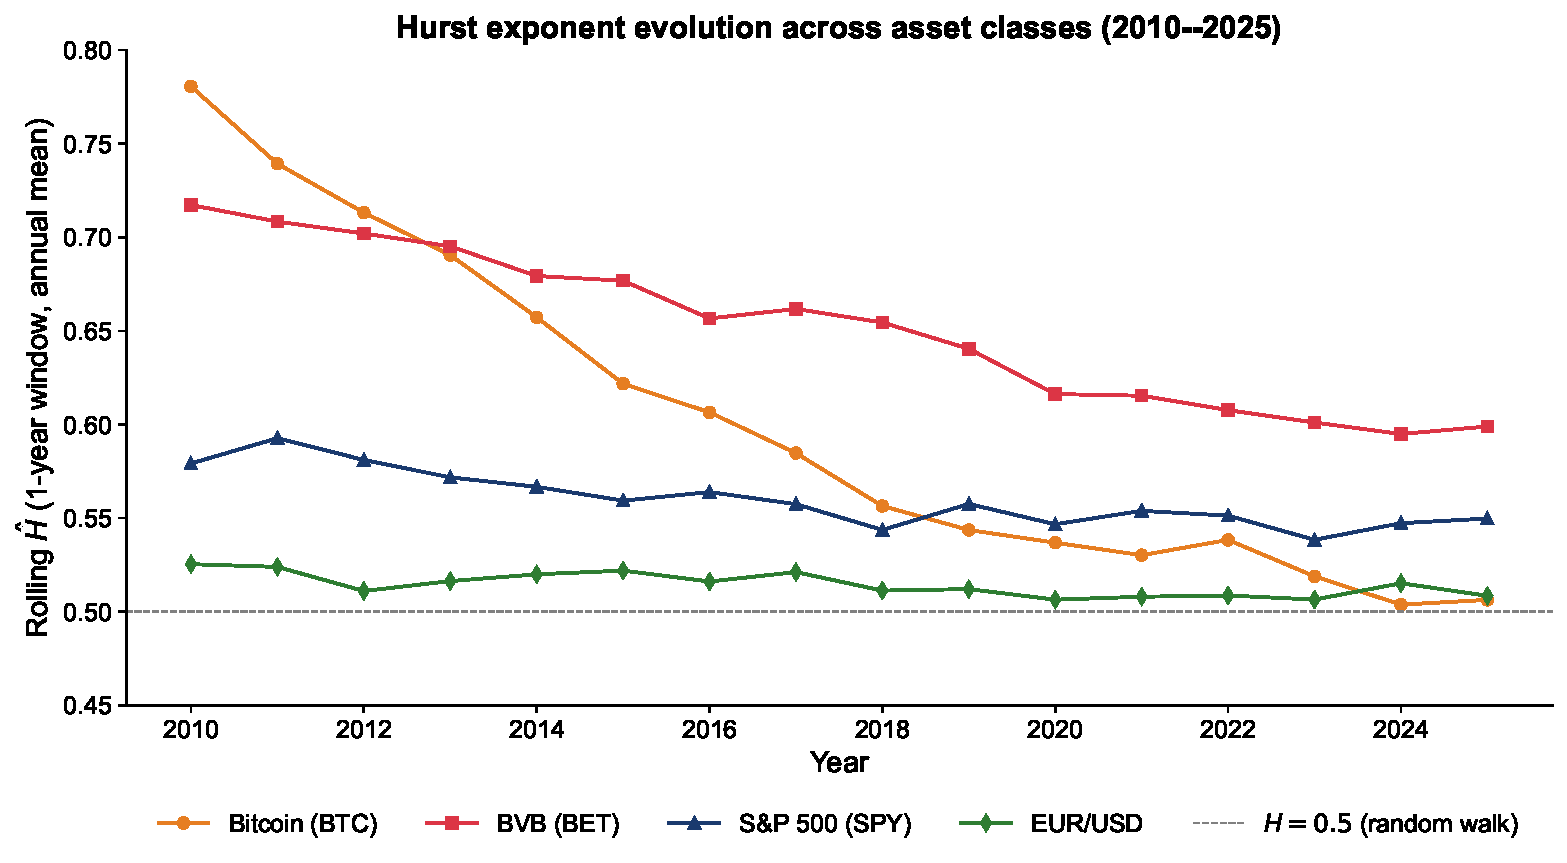
\includegraphics[width=\linewidth,height=4.4cm,keepaspectratio]{ch_fmh_eff_evolution.pdf}\\[1pt]
{\scriptsize\textcolor{MediumGray}{\textit{Evoluția eficienței pe Bitcoin (proxy: $|\hat H_t-0{,}5|$).}}}
\end{column}
\end{columns}
\vspace{0.1cm}
\begin{alertblock}{Particularități BTC}
\begin{itemize}\setlength{\itemsep}{0pt}
    \item Înjumătățirile (la fiecare 4 ani) $\Rightarrow$ ciclu fractal suplimentar
    \item Multifractalitate puternică, $f(\alpha)$ larg
    \item Mt.\ Gox 2014, interdicția din China 2017, Terra/FTX 2022 = resetări ale lui $\hat H$
\end{itemize}
\end{alertblock}
\end{cminipage}
\end{frame}

\begin{frame}[shrink=15]{Multifractalitate: spectrul $f(\alpha)$ pe Bitcoin}
\begin{cminipage}{0.95\textwidth}
\begin{columns}[T]
\begin{column}{0.55\textwidth}
\centering
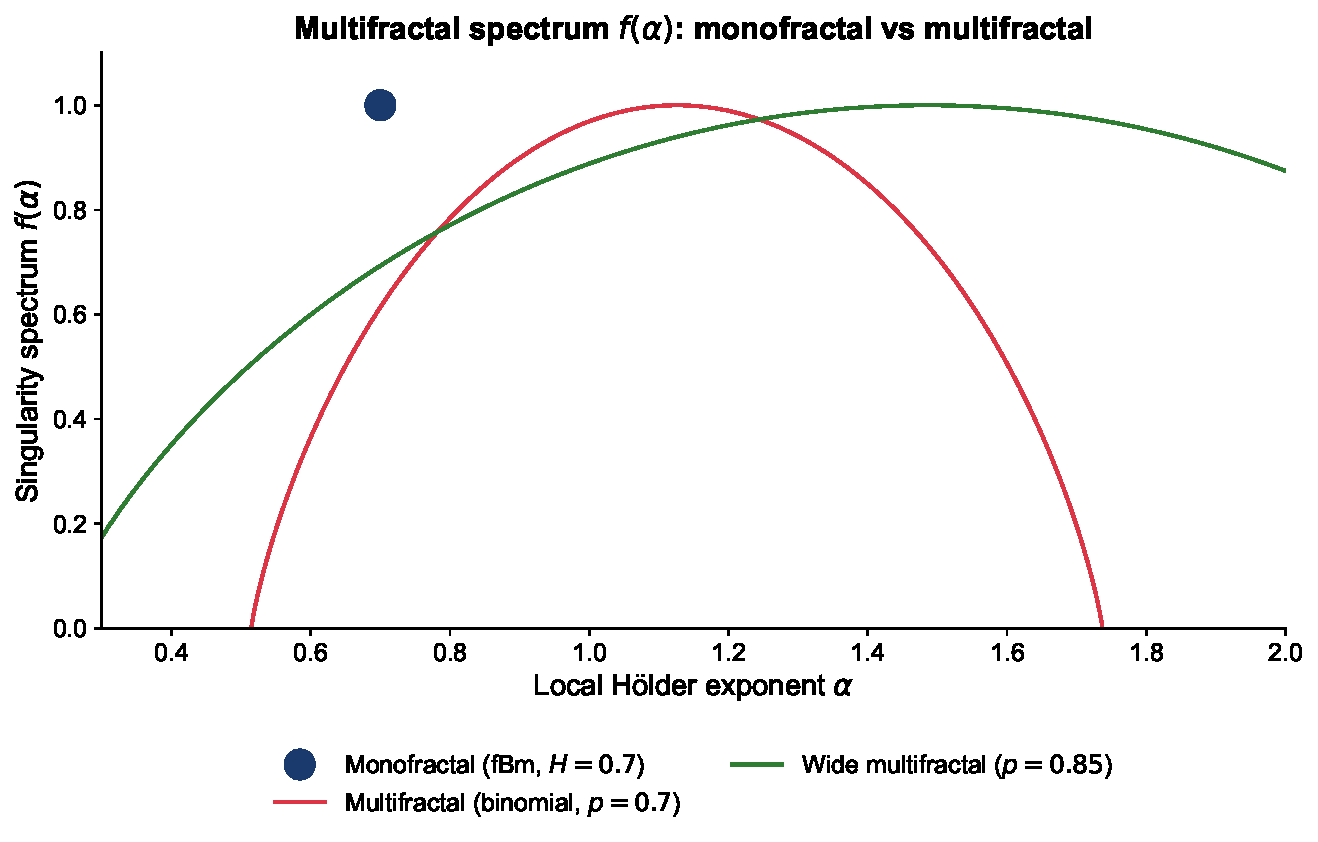
\includegraphics[width=\linewidth,height=4.4cm,keepaspectratio]{ch_fmh_spectrum.pdf}\\[1pt]
{\scriptsize\textcolor{MediumGray}{\textit{Spectrul multifractal $f(\alpha)$: monofractal (vârf îngust) vs multifractal (spectru larg).}}}
\end{column}
\begin{column}{0.42\textwidth}
\begin{block}{Ce ne spune $\Delta\alpha$?}
\begin{itemize}\setlength{\itemsep}{0pt}
    \item $\Delta\alpha=\alpha_{\max}-\alpha_{\min}$ = lățimea spectrului
    \item Mic $\Rightarrow$ aproape monofractal (un singur $H$)
    \item Mare $\Rightarrow$ multifractal puternic (multiple regimuri de scalare)
\end{itemize}
\end{block}
\begin{alertblock}{Aplicații practice}
\begin{itemize}\setlength{\itemsep}{0pt}
    \item $\Delta\alpha$ mare pe BTC, aur $\Rightarrow$ argument pentru testare la stres
    \item $\Delta\alpha$ mic pe FX $\Rightarrow$ aproape monofractal
\end{itemize}
\end{alertblock}
\end{column}
\end{columns}
\quantlet{SFM\_ch\_fmh\_extra: spectrum}{https://github.com/danpele/SFM/tree/main/Quantlets/SFM_ch_fmh}
\end{cminipage}
\end{frame}

\begin{frame}[shrink=15]{Recap §IV: 3 idei-cheie}
\begin{cminipage}{0.95\textwidth}
\begin{block}{De reținut}
\begin{enumerate}\setlength{\itemsep}{4pt}
    \item Piețe dezvoltate: $\hat H\approx 0{,}55$; emergente (BVB) $\hat H\approx 0{,}65$; cripto au $\hat H$ în declin pe măsură ce maturizează
    \item $\hat H>0{,}5$ NU implică profit garantat: persistența $\neq$ ineficiență exploatabilă
    \item Multifractalitatea (spectru larg $f(\alpha)$) oferă un cadru pentru a modela împreună aglomerarea volatilității, cozile grele și intermitența
\end{enumerate}
\end{block}
\begin{exampleblock}{Tranziție: \textit{,,acum trecem de la date reale la modelul stocastic''}}
\begin{itemize}\setlength{\itemsep}{0pt}
    \item §V: modelul stocastic generator --- fBm și multifractalitate
\end{itemize}
\end{exampleblock}
\end{cminipage}
\end{frame}

%#############################################################################
\section{Partea V: fBm și multifractalitate [CORE]}
%#############################################################################

\begin{frame}[shrink=15]{Mișcarea browniană standard (Wiener, 1923)}
\begin{cminipage}{0.95\textwidth}
\begin{defn}[Mișcarea browniană standard]
$\{B(t)\}_{t\geq 0}$ este procesul stocastic cu:
\begin{itemize}\setlength{\itemsep}{0pt}
    \item[(i)] $B(0)=0$
    \item[(ii)] incremenți \textbf{independenți}: $B(t)-B(s)\perp\!\!\!\perp B(u)-B(v)$ pentru intervale disjuncte
    \item[(iii)] incremenți \textbf{gaussieni}: $B(t)-B(s)\sim\mathcal{N}(0,\,t-s)$ pentru $0\leq s<t$
    \item[(iv)] traiectorii \textbf{continue} a.s.
\end{itemize}
\end{defn}
\begin{itemize}\setlength{\itemsep}{0pt}
    \item Autosimilaritate cu $H=1/2$: $B(ct)\stackrel{d}{=}c^{1/2}B(t)$
    \item Scalarea volatilității: $\sigma(\Delta)=\sigma(1)\sqrt{\Delta}$ (regula $\sqrt T$)
    \item Incremenți i.i.d.\ $\Rightarrow$ \textbf{fără memorie}; ACF $=0$ la orice lag $>0$
    \item Black--Scholes--Merton (1973): $dS_t=\mu S_t\,dt+\sigma S_t\,dB_t$ --- corespunde EMH în formă slabă
\end{itemize}
\end{cminipage}
\end{frame}

\begin{frame}[shrink=15]{fBm: definiția formală (Mandelbrot--Van Ness, 1968)}
\begin{cminipage}{0.95\textwidth}
\begin{defn}[Mișcarea browniană fracționară]
$\{B_H(t)\}_{t\in\R}$ cu $H\in(0,1)$ este unicul proces gaussian centrat cu $B_H(0)=0$ și covarianța
\[
    \E[B_H(t)B_H(s)]=\tfrac{1}{2}\bigl(|t|^{2H}+|s|^{2H}-|t-s|^{2H}\bigr).
\]
\end{defn}
\begin{columns}[T]
\begin{column}{0.50\textwidth}
\begin{itemize}\setlength{\itemsep}{0pt}
    \item Autosimilaritate: $B_H(ct)\stackrel{d}{=}c^H B_H(t)$
    \item Incremenți staționari, varianță $|t-s|^{2H}$
    \item $H=0{,}5$: mișcarea browniană standard
    \item $H>0{,}5$: persistent; $H<0{,}5$: anti-persistent
\end{itemize}
\end{column}
\begin{column}{0.46\textwidth}
\centering
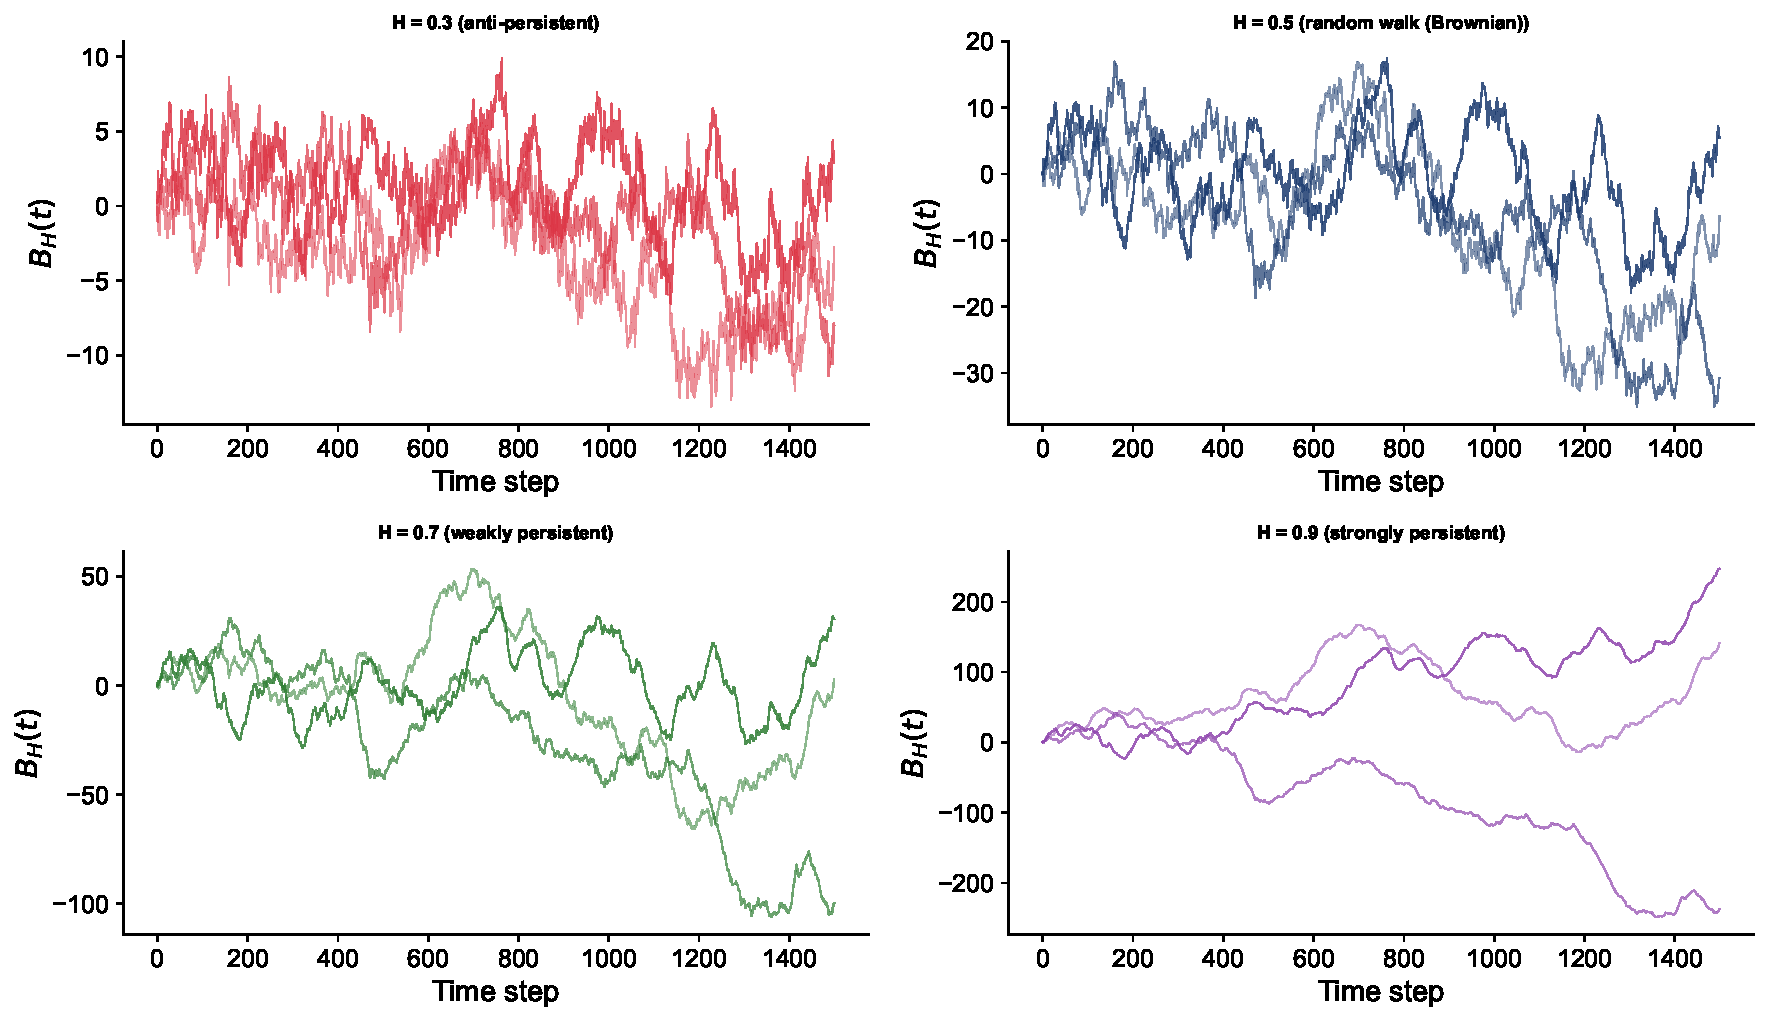
\includegraphics[height=3.8cm,keepaspectratio]{ch_fmh_fbm_paths.pdf}\\[1pt]
{\tiny\textcolor{MediumGray}{\textit{Traiectorii fBm: zimțate la $H=0{,}3$, netede la $H=0{,}9$.}}}
\end{column}
\end{columns}
\quantlet{SFM\_ch\_fmh\_fractals: fbm\_paths}{https://github.com/danpele/SFM/tree/main/Quantlets/SFM_ch_fmh}
\end{cminipage}
\end{frame}

\begin{frame}[shrink=15]{Proprietăți fBm: covarianță, varianță, simulare}
\begin{cminipage}{0.95\textwidth}
\begin{block}{Proprietăți cheie}
\begin{itemize}\setlength{\itemsep}{0pt}
    \item Varianță increment: $\E[(B_H(t+\tau)-B_H(t))^2]=\tau^{2H}$
    \item Sub $H=0{,}5$: regula clasică ,,varianța crește liniar cu timpul'' ($\Var\propto\tau$)
    \item Sub $H>0{,}5$: \textbf{varianța crește mai rapid decât liniar}
    \item Densitate spectrală a \textbf{incrementelor (fGn)}: $S(\omega)\sim |\omega|^{1-2H}$ când $\omega\to 0$ (zgomot $1/f^{\beta}$ cu $\beta=2H-1$)
\end{itemize}
\end{block}
\begin{exampleblock}{Calcul exemplu: $H=0{,}7$, $t=10$, $s=4$}
\begin{itemize}\setlength{\itemsep}{0pt}
    \item $|t|^{2H}=10^{1{,}4}\approx 25{,}12$
    \item $|s|^{2H}=4^{1{,}4}\approx 6{,}96$
    \item $|t-s|^{2H}=6^{1{,}4}\approx 12{,}29$
    \item $\E[B_H(10)B_H(4)]=\tfrac12(25{,}12+6{,}96-12{,}29)=\tfrac12\cdot 19{,}79\approx \mathbf{9{,}90}$
\end{itemize}
\end{exampleblock}
\begin{itemize}\setlength{\itemsep}{0pt}
    \item Simulare: \textbf{Davies--Harte} (FFT pe matrice circulantă) --- $O(N\log N)$
\end{itemize}
\end{cminipage}
\end{frame}

\begin{frame}[shrink=15]{fGn ca increment al fBm: ACF cu memorie lungă}
\begin{cminipage}{0.95\textwidth}
\begin{itemize}\setlength{\itemsep}{2pt}
    \item \textbf{Definiție}: $\xi_k=B_H(k+1)-B_H(k)$ --- \textbf{zgomot gaussian fracționar} (fGn)
    \item \textbf{Proprietăți}
    \begin{itemize}\setlength{\itemsep}{0pt}
        \item Staționar, gaussian, $\Var(\xi_k)=1$
        \item Autocorelație pe termen lung: $\rho(k)\sim H(2H-1)|k|^{2H-2}$
    \end{itemize}
    \item \textbf{Caz limită}
    \begin{itemize}\setlength{\itemsep}{0pt}
        \item $H=0{,}5$: fGn $=$ zgomot alb gaussian (incremenți i.i.d.)
        \item $H>0{,}5$: $\rho(k)>0$ și $\sum|\rho(k)|=\infty$ (\textbf{memorie lungă}!)
        \item $H<0{,}5$: $\rho(k)<0$ pentru $k\geq 1$ (anti-corelat)
    \end{itemize}
\end{itemize}
\centering
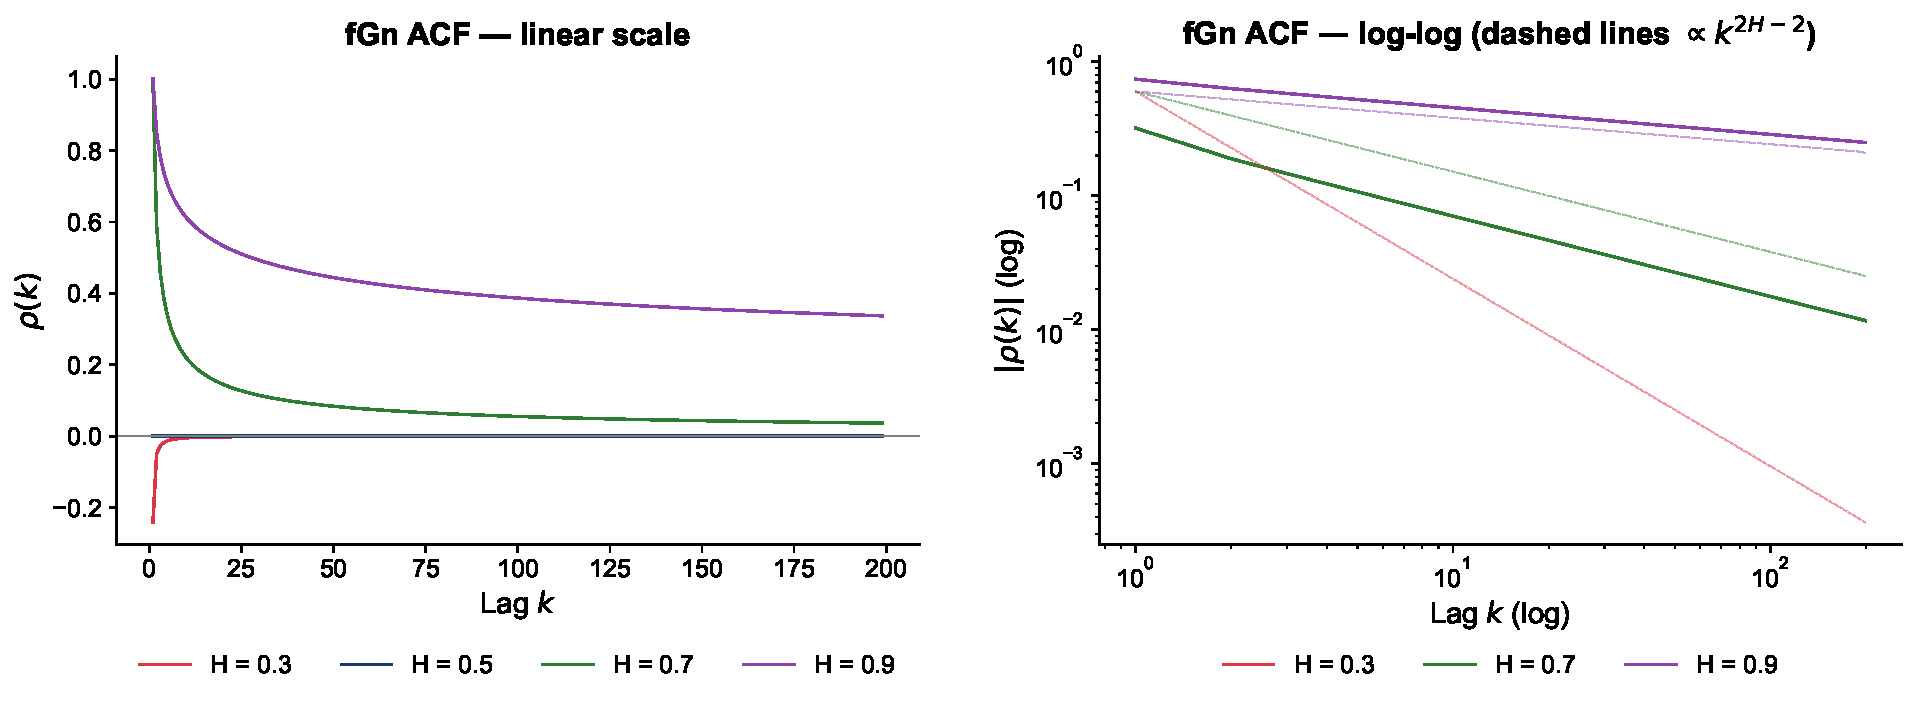
\includegraphics[width=0.56\linewidth,height=3.0cm,keepaspectratio]{ch_fmh_fgn_acf.pdf}\\[1pt]
{\scriptsize\textcolor{MediumGray}{\textit{ACF al fGn pentru $H\in\{0{,}3;\,0{,}5;\,0{,}7;\,0{,}9\}$.}}}
\quantlet{SFM\_ch\_fmh\_extra: fgn\_acf}{https://github.com/danpele/SFM/tree/main/Quantlets/SFM_ch_fmh}
\end{cminipage}
\end{frame}

\begin{frame}[shrink=15]{ARFIMA (\textit{AutoRegressive Fractionally Integrated Moving Average}): timp discret, $d=H-1/2$}
\begin{cminipage}{0.95\textwidth}
\begin{defn}[ARFIMA$(p,d,q)$]
$\Phi(L)(1-L)^d y_t=\Theta(L)\varepsilon_t$, cu $d\in(-1/2,1/2)$ parametru de \textbf{diferențiere fracționară}.
\end{defn}
\begin{itemize}\setlength{\itemsep}{0pt}
    \item \textbf{Conexiune cu fBm}: $d=H-1/2$
    \begin{itemize}\setlength{\itemsep}{0pt}
        \item ARFIMA = timp discret; fBm = timp continuu
    \end{itemize}
    \item \textbf{Proprietăți}
    \begin{itemize}\setlength{\itemsep}{0pt}
        \item $0<d<1/2$ $\Leftrightarrow$ memorie lungă, $H>1/2$
        \item Densitate spectrală: $f(\lambda)\sim C|\lambda|^{-2d}$ când $\lambda\to 0$
    \end{itemize}
\end{itemize}
\vspace{0.1cm}
\begin{exampleblock}{Operatorul $(1-L)^d$ pentru $d$ fracționar}
\begin{itemize}\setlength{\itemsep}{0pt}
    \item $(1-L)^d=\sum_{k=0}^\infty \binom{d}{k}(-L)^k$
    \item $\binom{d}{k}=\dfrac{d(d-1)\cdots(d-k+1)}{k!}$
    \item Coeficienții descresc \textbf{hiperbolic}, nu exponențial $\Rightarrow$ memorie lungă
\end{itemize}
\end{exampleblock}
\end{cminipage}
\end{frame}

\begin{frame}[shrink=15]{Memorie lungă vs scurtă: comparație vizuală}
\begin{cminipage}{0.95\textwidth}
\begin{columns}[T]
\begin{column}{0.55\textwidth}
\begin{block}{Memorie lungă ($d>0$, $H>1/2$)}
\begin{itemize}\setlength{\itemsep}{0pt}
    \item Decadere \textbf{hiperbolică}: $\rho(k)\sim k^{2d-1}$
    \item $\sum|\rho(k)|=\infty$
    \item Modele: ARFIMA, fBm, FIGARCH
\end{itemize}
\end{block}
\begin{block}{Memorie scurtă ($d=0$, ARMA)}
\begin{itemize}\setlength{\itemsep}{0pt}
    \item Decadere \textbf{exponențială}: $\rho(k)\sim\phi^k$
    \item $\sum|\rho(k)|<\infty$
    \item Modele: AR, MA, ARMA, GARCH
\end{itemize}
\end{block}
\end{column}
\begin{column}{0.43\textwidth}
\centering
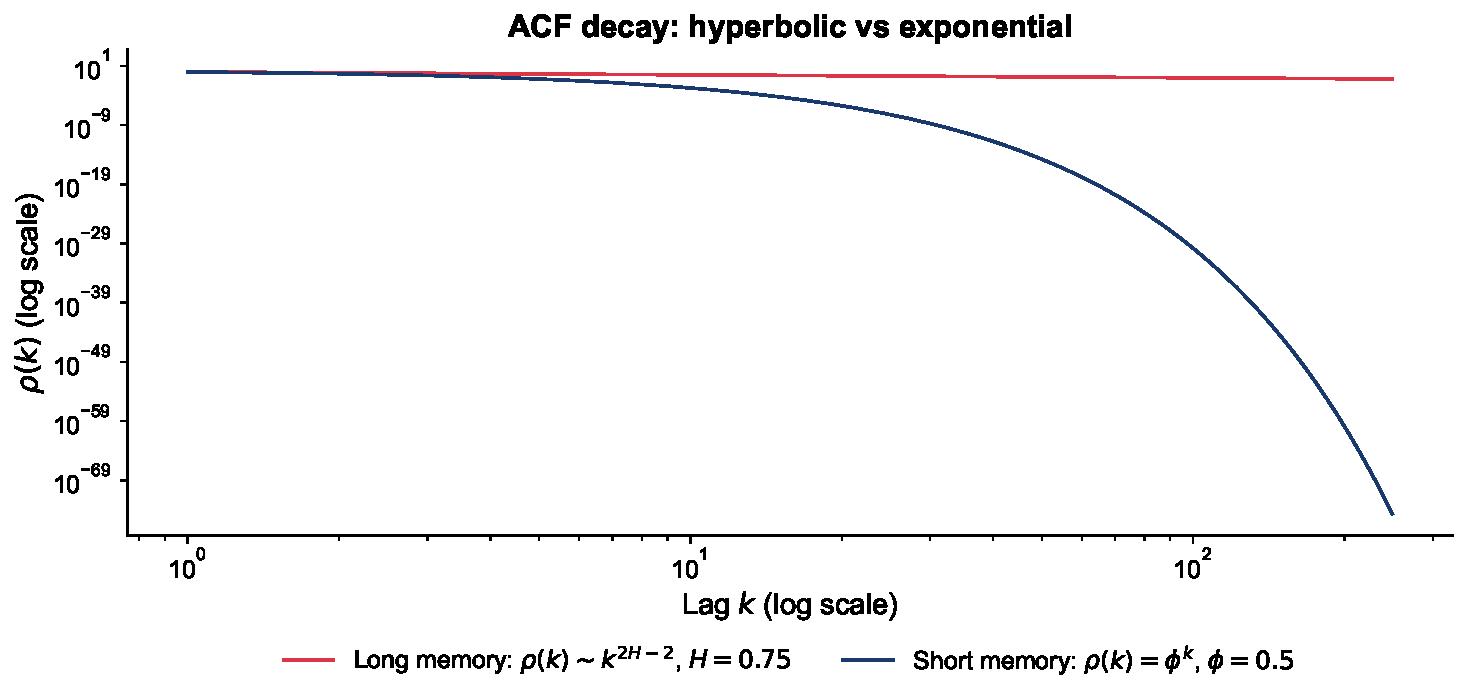
\includegraphics[width=\linewidth,height=4.4cm,keepaspectratio]{ch_fmh_lm_decay.pdf}\\[1pt]
{\scriptsize\textcolor{MediumGray}{\textit{ARFIMA/fBm vs AR(1) pe scală log-log.}}}
\end{column}
\end{columns}
\quantlet{SFM\_ch\_fmh\_extra: lm\_decay}{https://github.com/danpele/SFM/tree/main/Quantlets/SFM_ch_fmh}
\end{cminipage}
\end{frame}

\begin{frame}[shrink=15]{De la mono- la multifractalitate}
\begin{cminipage}{0.95\textwidth}
\begin{itemize}\setlength{\itemsep}{1pt}
    \item \textbf{Motivație}: un singur $H$ (\textbf{monofractal}) nu surprinde toate regimurile de scalare
    \item \textbf{Construcție formală}
    \begin{itemize}\setlength{\itemsep}{0pt}
        \item Procesul este \textbf{multifractal} dacă $\E[|X(t)|^q]=c(q)\cdot t^{\tau(q)+1}$ cu $\tau(q)$ \textbf{neliniar} în $q$
        \item Monofractal: $\tau(q)=qH-1$ (liniar)
        \item Spectrul multifractal $f(\alpha)$ = transformarea Legendre a $\tau(q)$
    \end{itemize}
    \item \textbf{Interpretare}
    \begin{itemize}\setlength{\itemsep}{0pt}
        \item Spectru \textbf{larg} $\Rightarrow$ multifractalitate puternică
        \item Surprinde simultan: aglomerarea volatilității, cozile grele și intermitența
    \end{itemize}
\end{itemize}
\vspace{0.1cm}
\begin{exampleblock}{Cum recunoaștem un multifractal}
\begin{itemize}\setlength{\itemsep}{0pt}
    \item MFDFA: estimează $h(q)$ pentru $q\in[-5,5]$
    \item Dacă $h(q)$ \textbf{depinde de $q$} $\Rightarrow$ multifractal
    \item Pe S\&P 500: $h(2)\approx 0{,}55$, $h(-2)\approx 0{,}65$ $\Rightarrow$ multifractalitate moderată
\end{itemize}
\end{exampleblock}
\end{cminipage}
\end{frame}

\begin{frame}[shrink=15]{Recap §V: 3 idei-cheie}
\begin{cminipage}{0.95\textwidth}
\begin{block}{De reținut}
\begin{enumerate}\setlength{\itemsep}{4pt}
    \item fBm = procesul gaussian central al FMH; $H$ controlează memoria, $H=0{,}5$ recuperează mișcarea browniană
    \item ARFIMA = analogul în timp discret, $d=H-1/2$; memoria lungă $\Leftrightarrow$ decadere hiperbolică a $\rho(k)$
    \item Multifractalitatea (MMAR) extinde monofractalul $\to$ spectru $f(\alpha)$ larg, surprinde mai bine aglomerarea volatilității și cozile grele
\end{enumerate}
\end{block}
\begin{exampleblock}{Tranziție: \textit{,,acum trecem de la diagnostic la risc''}}
\begin{itemize}\setlength{\itemsep}{0pt}
    \item §VI: implicații pentru \textbf{managementul riscului} --- VaR, ES, FIGARCH, volatilitate ,,rough''
\end{itemize}
\end{exampleblock}
\end{cminipage}
\end{frame}

%#############################################################################
\section{Partea VI: Managementul riscului sub FMH [CORE]}
%#############################################################################

\begin{frame}[shrink=15]{De ce contează FMH pentru managementul riscului?}
\begin{cminipage}{0.95\textwidth}
\begin{itemize}\setlength{\itemsep}{2pt}
    \item \textbf{Scalarea capitalului}
    \begin{itemize}\setlength{\itemsep}{0pt}
        \item Basel III, FRTB: regula clasică ,,$\sqrt T$'' presupune $H=0{,}5$
        \item Sub FMH: $\sigma_{T\text{-zile}}=\sigma_{1\text{-zi}}\cdot T^H$
    \end{itemize}
    \item \textbf{Aplicații operaționale}
    \begin{itemize}\setlength{\itemsep}{0pt}
        \item Detectarea regimului: $\hat H_t$ pe fereastră mobilă ca avertizare timpurie
        \item Alocarea portofoliului: $H$ mare $\Rightarrow$ urmărirea tendinței; $H$ mic $\Rightarrow$ strategie de tip contrar
        \item Testare la stres multifractală: scenarii cu spectru larg $f(\alpha)$
    \end{itemize}
\end{itemize}
\begin{exampleblock}{Idee-cheie}
\begin{itemize}\setlength{\itemsep}{0pt}
    \item Pe piețe persistente, ignorarea $H>0{,}5$ poate masca riscul latent pe orizonturi lungi
    \item VaR-ul scalat cu $T^H$ este util ca \textbf{instrument de testare la stres / diagnostic de sensibilitate}, nu ca substitut pentru cadrul Basel/FRTB
\end{itemize}
\end{exampleblock}
\end{cminipage}
\end{frame}

\begin{frame}[shrink=15]{Valoarea la risc (VaR, \textit{Value at Risk}) și pierderea așteptată (ES, \textit{Expected Shortfall}) sub memorie lungă: scalarea $T^H$}
\begin{cminipage}{0.95\textwidth}
\begin{block}{Formulă centrală}
\[
    \boxed{\;\text{VaR}_\alpha(T)\approx \mu T-\sigma\,T^H z_\alpha\;}
\]
\begin{itemize}\setlength{\itemsep}{0pt}
    \item Sub fBm: $\sigma(T)=\sigma(1)\,T^H$
    \item Diferența $T^H-\sqrt T$ (sensibilitate la $H\neq 0{,}5$) crește cu $T$ și cu $|H-0{,}5|$
\end{itemize}
\end{block}
\centering
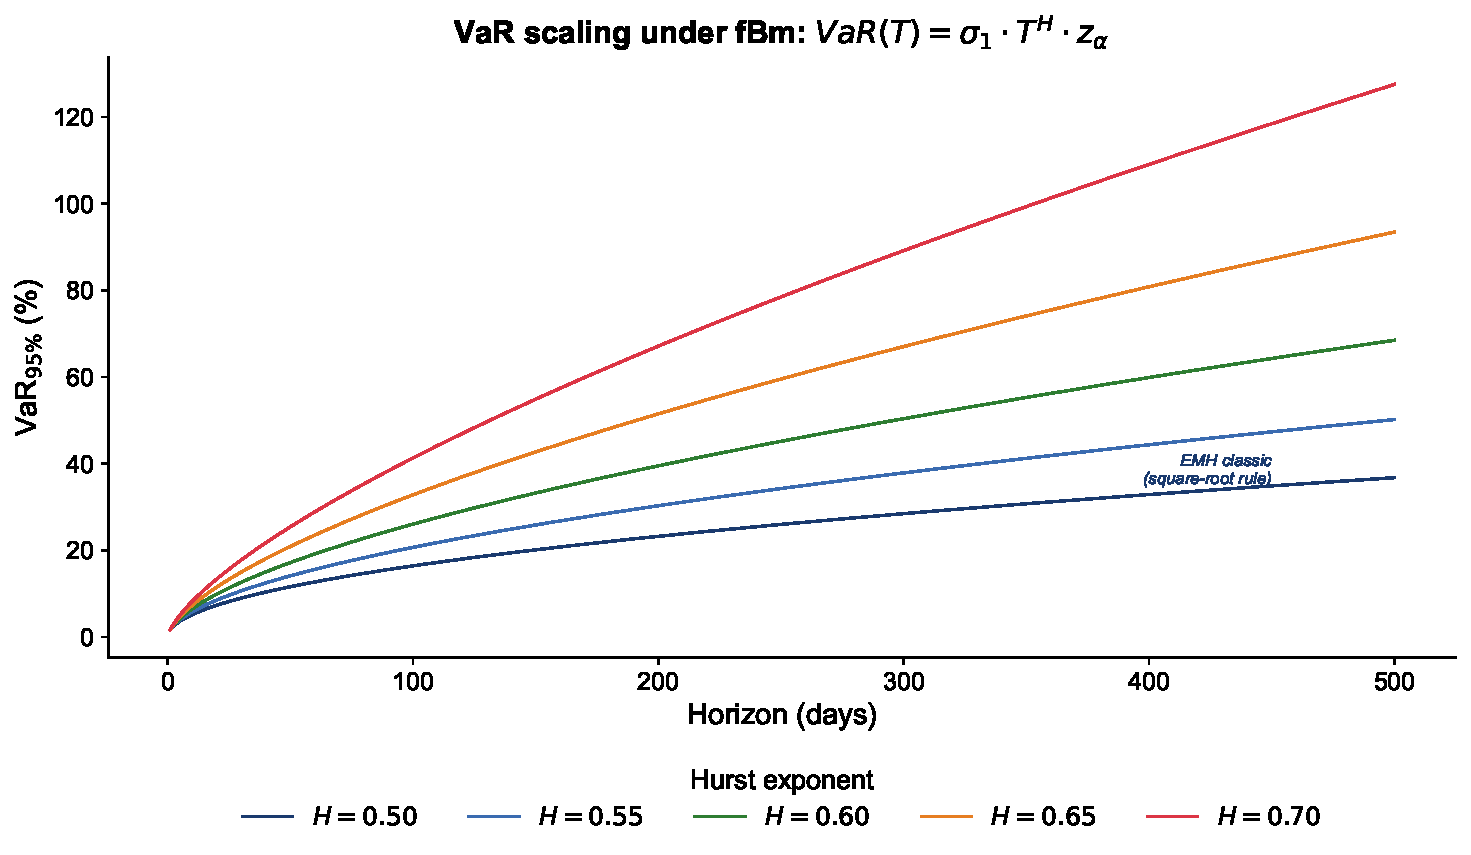
\includegraphics[width=0.56\linewidth,height=3.4cm,keepaspectratio]{ch_fmh_var_scaling.pdf}\\[1pt]
{\scriptsize\textcolor{MediumGray}{\textit{VaR$_{95\%}$ ca funcție de orizont $T$ pentru valori diferite ale $H$.}}}
\quantlet{SFM\_ch\_fmh\_extra: var\_scaling}{https://github.com/danpele/SFM/tree/main/Quantlets/SFM_ch_fmh}
\end{cminipage}
\end{frame}

\begin{frame}[shrink=25]{Mini-exercițiu D: $\sqrt T$ vs $T^H$ pe 22 zile}
\begin{cminipage}{0.95\textwidth}
\begin{block}{Sarcină}
\begin{itemize}\setlength{\itemsep}{0pt}
    \item Activ cu $\sigma_{1d}=1\%$, orizont $T=22$ zile (lună)
    \item Comparați $\sigma_{22d}$ sub $H=0{,}5$ ($\sqrt T$) și $H=0{,}6$ ($T^H$)
\end{itemize}
\end{block}
\begin{block}{Pași}
\begin{enumerate}\setlength{\itemsep}{0pt}
    \item Aplicați $\sigma_{Td}=\sigma_{1d}\cdot T^H$
    \item Substituiți $T=22$ și cele două valori ale lui $H$
    \item Calculați diferența procentuală relativă la $\sqrt T$
\end{enumerate}
\end{block}
\begin{exampleblock}{Răspuns}
\begin{itemize}\setlength{\itemsep}{0pt}
    \item (a) $\sigma_{22d}^{\sqrt T}=1\%\cdot 22^{0{,}5}\approx \mathbf{4{,}69\%}$
    \item (b) $\sigma_{22d}^{T^{0{,}6}}=1\%\cdot 22^{0{,}6}\approx \mathbf{6{,}45\%}$
    \item Diferență: $(6{,}45-4{,}69)/4{,}69\approx \mathbf{+38\%}$
\end{itemize}
\end{exampleblock}
\begin{alertblock}{Interpretare}
\begin{itemize}\setlength{\itemsep}{0pt}
    \item Acesta este un \textbf{exercițiu de sensibilitate} la ipoteza $H=0{,}5$, nu o corecție reglementară
    \item Folosit operațional ca test de stres alături de cadrul Basel/FRTB, nu ca substitut
\end{itemize}
\end{alertblock}
\end{cminipage}
\end{frame}

\begin{frame}[shrink=15]{Numere concrete: factor de scalare la 10 zile}
\begin{cminipage}{0.95\textwidth}
\begin{block}{Factorul de scalare al VaR pe 10 zile (orizont Basel)}
\renewcommand{\arraystretch}{1.25}
\centering
\begin{tabular}{lcc}
\toprule
\textbf{Ipoteză} & \textbf{Factor de scalare} & \textbf{Diferență vs $\sqrt T$} \\
\midrule
EMH ($H=0{,}5$): regula $\sqrt T$ & $10^{0{,}5}\approx 3{,}16$ & --- (referință) \\
FMH cu $H=0{,}55$ & $10^{0{,}55}\approx 3{,}55$ & $+12\%$ \\
FMH cu $H=0{,}60$ & $10^{0{,}60}\approx 3{,}98$ & $+26\%$ \\
FMH cu $H=0{,}65$ (BVB) & $10^{0{,}65}\approx 4{,}47$ & $+41\%$ \\
FMH cu $H=0{,}70$ & $10^{0{,}70}\approx 5{,}01$ & $+59\%$ \\
\bottomrule
\end{tabular}
\end{block}
\begin{alertblock}{Verdict}
\begin{itemize}\setlength{\itemsep}{0pt}
    \item Pe piețe persistente ($H>0{,}5$), regula $\sqrt T$ \textbf{subestimează} sensibilitatea volatilității la persistență
    \item În scenariul ipotetic $H=0{,}65$, factorul $T^H$ pe 10 zile este cu $\sim 41\%$ mai mare decât $\sqrt T$; diferența indică \textbf{sensibilitatea capitalului la persistență}, nu o corecție reglementară directă
\end{itemize}
\end{alertblock}
\end{cminipage}
\end{frame}

\begin{frame}[shrink=15]{Sensibilitatea $T^H$ vs.\ $\sqrt T$ pe diferite orizonturi}
\begin{cminipage}{0.95\textwidth}
\renewcommand{\arraystretch}{1.2}
\centering
\small
\begin{tabular}{lccc}
\toprule
\textbf{Orizont $T$} & \textbf{$T^{0{,}5}$} & \textbf{$T^{0{,}65}$} & \textbf{Diferență relativă} \\
\midrule
1 zi & 1,00 & 1,00 & 0\% \\
5 zile & 2,24 & 2,87 & $+28\%$ \\
10 zile & 3,16 & 4,47 & $+41\%$ \\
22 zile (lună) & 4,69 & 7,29 & $+55\%$ \\
65 zile (trim.) & 8,06 & 14,79 & $+83\%$ \\
252 zile (an) & 15,87 & 39,81 & $+151\%$ \\
\bottomrule
\end{tabular}
\vspace{0.15cm}
\begin{exampleblock}{Lecție --- ca analiză de sensibilitate}
\begin{itemize}\setlength{\itemsep}{0pt}
    \item Discrepanța $\sqrt T$ vs.\ $T^H$ \textbf{crește cu orizontul $T$}
    \item Pe un an, pentru o serie cu $H\approx 0{,}65$ (scenariu ipotetic), $T^H$ depășește $\sqrt T$ cu peste $150\%$ --- măsură a sensibilității la persistență, nu corecție reglementară
    \item \textbf{Interpretare prudentă}: $T^H$ rămâne un \textbf{exercițiu de sensibilitate / diagnostic de stres}, nu un înlocuitor al cadrului Basel/FRTB
\end{itemize}
\end{exampleblock}
\end{cminipage}
\end{frame}

\begin{frame}[shrink=15]{Procedură standard de analiză fractală}
\begin{cminipage}{0.95\textwidth}
\begin{block}{Procedură în 6 pași: date $\to$ $\hat H$ $\to$ regim $\to$ risc}
\begin{enumerate}\setlength{\itemsep}{2pt}
    \item \textbf{Date}: log-randamente $r_t=\ln P_t-\ln P_{t-1}$
    \item \textbf{Estimarea} lui $\hat H$ prin DFA-1 (sau Lo R/S pentru testul formal)
    \item \textbf{Test} $H_0:H=0{,}5$ prin Variance Ratio
    \item \textbf{Verificarea regimului}: $\hat H_t$ pe fereastră mobilă + puncte de ruptură Bai--Perron
    \item \textbf{Multifractal} (opțional): MFDFA pentru $h(q),f(\alpha)$
    \item \textbf{Risc}: VaR/ES cu scalare $T^H$; alocare în funcție de regim
\end{enumerate}
\end{block}
\begin{exampleblock}{Rezultat minim de raportat}
\begin{itemize}\setlength{\itemsep}{0pt}
    \item Tabel cu $\hat H_{\text{DFA}}$, $\hat H_{\text{LoRS}}$, statistica VR + interval de încredere bootstrap
    \item Grafic al lui $\hat H_t$ pe fereastră mobilă (252 zile) cu benzi de încredere
    \item Eventual: grafic $h(q)$ și spectrul $f(\alpha)$
    \item VaR$_{99\%}$ pe 10 zile: comparativ EMH vs FMH
\end{itemize}
\end{exampleblock}
\end{cminipage}
\end{frame}

\begin{frame}[shrink=15]{Recap §VI: 3 idei-cheie}
\begin{cminipage}{0.95\textwidth}
\begin{block}{De reținut}
\begin{enumerate}\setlength{\itemsep}{4pt}
    \item Sub FMH: $\sigma(T)=\sigma(1)T^H$ în loc de $\sqrt T$; pentru $H\in[0{,}55;\,0{,}65]$, factorul $T^H$ depășește $\sqrt T$ cu $\sim 12$--$41\%$ pe orizont 10z (sensibilitate la persistență, nu corecție reglementară)
    \item FIGARCH/HAR pentru memoria lungă în volatilitate; volatilitate ,,rough'' ($H\approx 0{,}1$) pentru opțiuni
    \item Procedură operațională: DFA $\to$ test $H=0{,}5$ $\to$ estimare mobilă $\to$ MFDFA $\to$ recalibrarea riscului
\end{enumerate}
\end{block}
\begin{exampleblock}{Tranziție: \textit{,,acum trecem de la procedură la crize reale''}}
\begin{itemize}\setlength{\itemsep}{0pt}
    \item §VII: aplicăm procedura pe \textbf{crize reale} --- 1987, 2008, COVID-19, BVB, Bitcoin
\end{itemize}
\end{exampleblock}
\end{cminipage}
\end{frame}

%#############################################################################
\section{Partea VII: Studii de caz --- crize [CORE]}
%#############################################################################

\begin{frame}[shrink=15]{Hurst pe fereastră mobilă ca semnal de avertizare: 3 crize}
\begin{cminipage}{0.95\textwidth}
\renewcommand{\arraystretch}{1.2}
\centering
\small
\begin{tabular}{llll}
\toprule
\textbf{Criză} & \textbf{$\hat H_t$ înainte} & \textbf{$\hat H_t$ în criză} & \textbf{Mecanism FMH} \\
\midrule
Black Monday (1987) & $\sim 0{,}55$ & $\to 0{,}50$ & Asigurare portofoliu + tranzacționare programată \\
Criza financiară 2008 (Lehman) & $\sim 0{,}55$ & $\to 0{,}48$ & Investitorii ,,long-only''/value pleacă, rămân HFT \\
COVID-19 (mart.\ 2020) & $\sim 0{,}58$ & $\to 0{,}40$ & Vânzare/cumpărare frenetică, anti-persistență \\
\bottomrule
\end{tabular}
\vspace{0.2cm}
\begin{block}{Diagnostic FMH comun}
\begin{itemize}\setlength{\itemsep}{0pt}
    \item Un șoc fundamental afectează simultan toate orizonturile
    \item Investitorii pe termen lung adoptă comportament pe termen scurt (vânzare în panică)
    \item Distribuția orizonturilor \textbf{colapsează} $\Rightarrow$ \textbf{lichiditatea dispare}
    \item Structura fractală se rupe $\Rightarrow$ $\hat H_t$ se schimbă brusc spre/sub $0{,}5$
\end{itemize}
\end{block}
\end{cminipage}
\end{frame}

\begin{frame}[shrink=15]{Black Monday 1987}
\begin{cminipage}{0.95\textwidth}
\begin{block}{Context}
\begin{itemize}\setlength{\itemsep}{0pt}
    \item 19 oct.\ 1987: DJIA $-22{,}6\%$ într-o singură zi --- cea mai mare cădere zilnică din istoric
    \item Volume de $4\times$ media zilnică, fără un șoc fundamental identificabil
    \item Cauze tehnice: asigurare de portofoliu + tranzacționare programată
\end{itemize}
\end{block}
\begin{alertblock}{Diagnostic FMH}
\begin{itemize}\setlength{\itemsep}{0pt}
    \item $\hat H_t$ trece de la $\approx 0{,}55$ (înainte) la $\approx 0{,}50$ în octombrie 1987
    \item \textbf{Colapsul orizonturilor}: asigurarea de portofoliu îi forțează pe investitorii pe termen lung să adopte comportament tip HFT
    \item Probabilitate sub gauss $\sim 10^{-50}$ --- imposibil sub etalonul EMH
\end{itemize}
\end{alertblock}
\begin{exampleblock}{Lecție pentru risc}
\begin{itemize}\setlength{\itemsep}{0pt}
    \item Mecanisme de oprire automată (circuit breakers) introduse de NYSE în 1988; pragurile actuale $-7\%/-13\%/-20\%$ pe S\&P~500 datează din februarie 2013
    \item Sub FMH: pauza forțată = restaurarea diversității orizonturilor
    \item Diagnostic operațional: monitorizați $\hat H_t$ + diversitatea cohortelor de investitori
\end{itemize}
\end{exampleblock}
\end{cminipage}
\end{frame}

\begin{frame}[shrink=15]{Criza Financiară Globală 2008 (GFC, \textit{Global Financial Crisis})}
\begin{cminipage}{0.95\textwidth}
\begin{block}{Context}
\begin{itemize}\setlength{\itemsep}{0pt}
    \item aug.\ 2007: BNP Paribas îngheață fonduri MBS; 15 sep.\ 2008: Lehman depune Chapter 11
    \item Indici globali $-40\%$ în 6 luni; VIX$\to 80$
    \item Răspuns: TARP \$700~mld., QE al Fed
\end{itemize}
\end{block}
\begin{alertblock}{Diagnostic FMH}
\begin{itemize}\setlength{\itemsep}{0pt}
    \item $\hat H$ pe S\&P~500 scade de la $\sim 0{,}55$ la $\sim 0{,}48$
    \item Investitorii ,,long-only''/value pleacă; rămân predominant HFT $\Rightarrow$ lichiditatea scade abrupt
    \item Depășiri ale VaR cu mult peste așteptările modelului gaussian
\end{itemize}
\end{alertblock}
\begin{exampleblock}{Lecție pentru risc}
\begin{itemize}\setlength{\itemsep}{0pt}
    \item GFC = primul caz documentat empiric în care $\hat H_t$ a fost folosit ca semnal de avertizare timpurie
    \item Dominique \& Rivera (2011): $\hat H_t$ a scăzut spre $0{,}48$ cu $\sim$3 luni înainte de Lehman
    \item Revenire în formă de U pe 18 luni $\Rightarrow$ recalibrarea limitelor de capital pe orizonturi multiple
\end{itemize}
\end{exampleblock}
\end{cminipage}
\end{frame}

\begin{frame}[shrink=15]{COVID-19 (martie 2020)}
\begin{cminipage}{0.95\textwidth}
\begin{block}{Context}
\begin{itemize}\setlength{\itemsep}{0pt}
    \item 11 mar.\ 2020: OMS declară pandemie; 12 mar.\ S\&P~500 $-9{,}5\%$, 16 mar.\ $-12\%$
    \item Cea mai rapidă scădere accentuată din istorie: $-34\%$ în 33 zile
    \item 23 mar.: Fed lansează QE fără limită
\end{itemize}
\end{block}
\begin{alertblock}{Diagnostic FMH}
\begin{itemize}\setlength{\itemsep}{0pt}
    \item $\hat H_t$ trece de la $\approx 0{,}58$ la $\approx 0{,}40$ în două săptămâni
    \item Anti-persistență temporară ($H<0{,}5$): vânzare/cumpărare frenetică
    \item Revine la $\approx 0{,}55$ în iulie 2020 --- cea mai rapidă tranziție de regim Hurst observată
\end{itemize}
\end{alertblock}
\begin{exampleblock}{Lecție pentru risc}
\begin{itemize}\setlength{\itemsep}{0pt}
    \item COVID a comprimat în zile ceea ce în 2008 a durat luni $\Rightarrow$ recalibrare urgentă a limitelor de risc
    \item Asimetrie cădere/revenire (V vs.\ U în 2008) --- model de stres adecvat: stimul fiscal-monetar imediat
    \item Implicație operațională: ferestre mobile mai scurte (50--100 zile) pentru detectarea regimului în crize rapide
\end{itemize}
\end{exampleblock}
\end{cminipage}
\end{frame}

\begin{frame}[shrink=15]{BVB: promovare la \textit{Emerging Market} (FTSE, sept.\ 2020)}
\begin{cminipage}{0.95\textwidth}
\begin{block}{Context}
\begin{itemize}\setlength{\itemsep}{0pt}
    \item BET = primii 21 emitenți de la BVB; surse: Pele \& Mazurencu (2014), Tilfani \& El~Boukfaoui (2020)
    \item $\hat H_{\text{BET}}\in[0{,}60;\,0{,}72]$ înainte de 2020
    \item 21 sept.\ 2020: FTSE promovează BVB la statut de \textit{Emerging Market}
\end{itemize}
\end{block}
\begin{alertblock}{Diagnostic FMH}
\begin{itemize}\setlength{\itemsep}{0pt}
    \item Pre-promovare: $\hat H\approx 0{,}68$ (lichiditate redusă, retail dominant, concentrare pe puțini emitenți)
    \item Post-promovare: $\hat H\approx 0{,}62$ (volume $\uparrow$, investitori instituționali străini $\uparrow$)
    \item Mecanism: diversitate de orizonturi $\uparrow$ $\Rightarrow$ $\hat H\to 0{,}5$ (maturizare)
\end{itemize}
\end{alertblock}
\begin{exampleblock}{Lecție pentru risc}
\begin{itemize}\setlength{\itemsep}{0pt}
    \item Predicția FMH se confirmă pe BVB: lichiditate $\uparrow$ $\Rightarrow$ eficiență $\uparrow$ $\Rightarrow$ $H\to 0{,}5$
    \item Pe piețe cu $H>0{,}55$ persistent, scalarea $T^H$ rămâne un diagnostic util de stres
    \item Monitorizați $\hat H_t$ după evenimente structurale (promovare, ETF nou, listări mari)
\end{itemize}
\end{exampleblock}
\end{cminipage}
\end{frame}

\begin{frame}[shrink=15]{Bitcoin: analiză aprofundată a evoluției eficienței}
\begin{cminipage}{0.95\textwidth}
\begin{block}{Context}
\begin{itemize}\setlength{\itemsep}{0pt}
    \item 2010--2014 (incipient): $\hat H\approx 0{,}70$--$0{,}80$
    \item 2015--2018 (maturizare): $\approx 0{,}55$--$0{,}65$ (futures CME, dec.\ 2017)
    \item 2019--prezent: $\approx 0{,}50$--$0{,}55$ (ETF spot, ian.\ 2024); resetări la Mt.\ Gox 2014, China 2017, Terra/FTX 2022
\end{itemize}
\end{block}
\begin{alertblock}{Diagnostic FMH}
\begin{itemize}\setlength{\itemsep}{0pt}
    \item Tranziție clasică: piață ineficientă $\to$ cvasi-eficientă, similară cu FX
    \item Multifractalitate puternică ($f(\alpha)$ larg) + ciclul fractal al înjumătățirii (4 ani)
    \item Tranzacționare 24/7 $\Rightarrow$ rezoluție temporală fină pentru $\hat H_t$
\end{itemize}
\end{alertblock}
\begin{exampleblock}{Lecție pentru risc}
\begin{itemize}\setlength{\itemsep}{0pt}
    \item Dacă tendința continuă, $\hat H_{\text{BTC}}\to 0{,}50$ (similar cu FX) --- predicție condiționată de lichiditate și diversitate
    \item Pentru testarea la stres a portofoliilor cripto: combină $T^H$ cu spectrul $f(\alpha)$ pentru evenimente extreme
    \item Monitorizați $\hat H_t$ în jurul evenimentelor structurale (ETF spot, halving, falimente burse)
\end{itemize}
\end{exampleblock}
\end{cminipage}
\end{frame}

\begin{frame}[shrink=15]{Flash Crash 2010: criza de 36 de minute}
\begin{cminipage}{0.95\textwidth}
\begin{block}{Context}
\begin{itemize}\setlength{\itemsep}{0pt}
    \item 6 mai 2010, 14:32 ET: vânzare automată a 75.000 contracte E-mini S\&P~500
    \item 14:42--14:47: DJIA $-9{,}16\%$ (998 puncte); 14:48--15:08: revenire aproape totală
    \item Cauză tehnică: algoritm VWAP fără limite de viteză $\to$ HFT-urile se retrag $\to$ vid de lichiditate
\end{itemize}
\end{block}
\begin{alertblock}{Diagnostic FMH}
\begin{itemize}\setlength{\itemsep}{0pt}
    \item Colapsul orizonturilor în \textbf{minute}, nu zile
    \item $\hat H_t$ intra-zi atinge $\sim 0{,}3$ în minutul de vârf
    \item Anti-persistență extremă: alternanță vânzare $\to$ cumpărare la frecvențe foarte înalte
\end{itemize}
\end{alertblock}
\begin{exampleblock}{Lecție pentru risc}
\begin{itemize}\setlength{\itemsep}{0pt}
    \item Mecanismul \textit{Limit Up--Limit Down} (LULD), implementat de SEC în aprilie 2013: pauze la $\pm 5\%$ pentru titlurile din Tier~1
    \item Mini-întrerupătoare la nivel de acțiune $\Rightarrow$ restaurarea forțată a diversității
    \item Implicație pentru execuție: limitare automată a vitezei pentru ordine mari
\end{itemize}
\end{exampleblock}
\end{cminipage}
\end{frame}

\begin{frame}[shrink=15]{Șablon comun pentru studiile de caz}
\begin{cminipage}{0.95\textwidth}
\begin{block}{Cele 4 întrebări obligatorii pentru fiecare criză}
\begin{enumerate}\setlength{\itemsep}{3pt}
    \item \textbf{Context}: cronologie, factori declanșatori, magnitudine ($\Delta P,\Delta\sigma,\Delta$ vol.)
    \item \textbf{Ce măsurăm}: seria folosită (frecvență, perioadă), metoda ($\hat H$ pe fereastră mobilă, DFA, MFDFA)
    \item \textbf{Ce arată $\hat H_t$/DFA/MFDFA}: profilul lui $\hat H_t$ (cădere, anti-persistență, multifractalitate $\Delta\alpha$)
    \item \textbf{Implicație pentru risc}: depășiri ale VaR, lichiditate, acoperire (hedging), reglementare
\end{enumerate}
\end{block}
\begin{exampleblock}{Idee}
\begin{itemize}\setlength{\itemsep}{0pt}
    \item Acest șablon asigură \textbf{comparabilitatea} între crize
    \item Conectează diagnosticul fractal cu deciziile de management al riscului
    \item Aplicabil și crizelor istorice (1929, Asia 1997, Flash Crash 2010, GameStop 2021, SVB 2023)
\end{itemize}
\end{exampleblock}
\end{cminipage}
\end{frame}

\begin{frame}[shrink=15]{Recap §VII: 3 idei-cheie}
\begin{cminipage}{0.95\textwidth}
\begin{block}{De reținut}
\begin{enumerate}\setlength{\itemsep}{4pt}
    \item Piețe dezvoltate au $\hat H\approx 0{,}55$; piețe emergente (BVB) $\hat H\approx 0{,}65$; cripto au $\hat H$ în declin pe măsură ce maturizează
    \item $\hat H_t$ pe fereastră mobilă a marcat 1987, 2008 și COVID-19 printr-un colaps observabil spre/sub $0{,}5$ (potențial semnal de avertizare timpurie; pentru 2008, Dominique \& Rivera 2011 arată o cădere cu $\sim$3 luni înainte de prăbușirea Lehman)
    \item BVB ilustrează predicția FMH: lichiditate $\uparrow$ $\Rightarrow$ diversitate orizonturi $\uparrow$ $\Rightarrow$ $\hat H\to 0{,}5$
\end{enumerate}
\end{block}
\begin{exampleblock}{Tranziție: \textit{,,acum trecem de la teorie la exerciții de examen''}}
\begin{itemize}\setlength{\itemsep}{0pt}
    \item §VIII: exerciții de examen cu rezolvare detaliată
\end{itemize}
\end{exampleblock}
\end{cminipage}
\end{frame}

%#############################################################################
\section{Partea VIII: Exerciții de examen [EXERCIȚII]}
%#############################################################################

\begin{frame}[shrink=15]{Exercițiul 1: dimensiune Sierpinski carpet}
\begin{cminipage}{0.95\textwidth}
\begin{block}{Enunț}
\begin{itemize}\setlength{\itemsep}{0pt}
    \item Considerăm fractalul \textit{Sierpinski carpet}: pătratul unitate este împărțit în 9 pătrate egale și se elimină pătratul central; procedeul se repetă pe fiecare dintre cele 8 pătrate rămase.
\end{itemize}
\end{block}
\begin{itemize}\setlength{\itemsep}{0pt}
    \item \textbf{Cerințe}
    \begin{itemize}\setlength{\itemsep}{0pt}
        \item Calculați dimensiunea de similaritate $D$
        \item Comparați cu pătratul plin ($D=2$) și triunghiul Sierpinski ($D=\log 3/\log 2$)
        \item Dacă graficul prețului ar avea această dimensiune, ce $\hat H$ ar corespunde (din $D=2-H$)?
    \end{itemize}
\end{itemize}
\end{cminipage}
\end{frame}

\begin{frame}[shrink=15]{Exercițiul 1: Rezolvare}
\begin{cminipage}{0.95\textwidth}
\begin{exampleblock}{Rezolvare}
\begin{itemize}\setlength{\itemsep}{0pt}
    \item \textbf{Identificare $N$ și $r$}
    \begin{itemize}\setlength{\itemsep}{0pt}
        \item Din 9 pătrate, rămân $N=8$ copii
        \item Scara fiecărei copii: $r=1/3$, deci $s=3$
    \end{itemize}
    \item \textbf{Dimensiunea de similaritate}
    \begin{itemize}\setlength{\itemsep}{0pt}
        \item $D=\dfrac{\log N}{\log s}=\dfrac{\log 8}{\log 3}=\dfrac{3\log 2}{\log 3}\approx \mathbf{1{,}893}$
    \end{itemize}
    \item \textbf{Comparație}
    \begin{itemize}\setlength{\itemsep}{0pt}
        \item Pătrat plin: $D=2$ (umple planul)
        \item Sierpinski carpet: $D\approx 1{,}893$ (aproape de plan, dar are găuri)
        \item Sierpinski triangle: $D=\log 3/\log 2\approx 1{,}585$ (mai puține pătrate)
    \end{itemize}
    \item \textbf{Translatare la prețuri}
    \begin{itemize}\setlength{\itemsep}{0pt}
        \item Dacă $D=1{,}893$, atunci $\hat H=2-D\approx 0{,}107$
        \item Aceasta este zona ,,rough volatility'' (Gatheral, Jaisson, Rosenbaum, 2018)
        \item Volatilitate intraday tipic are $H\approx 0{,}1$
    \end{itemize}
\end{itemize}
\end{exampleblock}
\end{cminipage}
\end{frame}

\begin{frame}[shrink=15]{Exercițiul 2: R/S pe serie scurtă}
\begin{cminipage}{0.95\textwidth}
\begin{block}{Enunț}
\begin{itemize}\setlength{\itemsep}{0pt}
    \item Pentru seria $x=\{2;\,4;\,1;\,5;\,3;\,7;\,2;\,4\}$ ($n=8$):
\end{itemize}
\end{block}
\begin{itemize}\setlength{\itemsep}{0pt}
    \item \textbf{Cerințe}
    \begin{itemize}\setlength{\itemsep}{0pt}
        \item Calculați $\bar x$ și seria cumulată $Y_k=\sum_{i=1}^k(x_i-\bar x)$
        \item Calculați $R=\max Y-\min Y$ și $S=\sigma(x)$
        \item Calculați raportul $R/S$ pentru $n=8$
        \item Estimarea $\hat H$ ar necesita ce alte mărimi de bloc?
    \end{itemize}
\end{itemize}
\end{cminipage}
\end{frame}

\begin{frame}[shrink=15]{Exercițiul 2: Rezolvare}
\begin{cminipage}{0.95\textwidth}
\begin{exampleblock}{Rezolvare}
\begin{itemize}\setlength{\itemsep}{0pt}
    \item \textbf{Media}
    \begin{itemize}\setlength{\itemsep}{0pt}
        \item $\bar x=(2+4+1+5+3+7+2+4)/8=28/8=\mathbf{3{,}5}$
    \end{itemize}
    \item \textbf{Cumulate $Y_k$ (deviații: $\{-1{,}5;\,0{,}5;\,-2{,}5;\,1{,}5;\,-0{,}5;\,3{,}5;\,-1{,}5;\,0{,}5\}$)}
    \begin{itemize}\setlength{\itemsep}{0pt}
        \item $Y=\{-1{,}5;\,-1{,}0;\,-3{,}5;\,-2{,}0;\,-2{,}5;\,1{,}0;\,-0{,}5;\,0\}$
    \end{itemize}
    \item \textbf{$R$ și $S$}
    \begin{itemize}\setlength{\itemsep}{0pt}
        \item $R=\max Y-\min Y=1{,}0-(-3{,}5)=\mathbf{4{,}5}$
        \item Varianța (cu $n$): $\sum(x_i-\bar x)^2/n=25{,}75/8\approx 3{,}219$
        \item $S=\sqrt{3{,}219}\approx \mathbf{1{,}794}$
    \end{itemize}
    \item \textbf{Raportul}: $R/S=4{,}5/1{,}794\approx \mathbf{2{,}51}$ pentru $n=8$
    \item \textbf{Pentru regresie}
    \begin{itemize}\setlength{\itemsep}{0pt}
        \item Repetă pentru $n=4$ (2 blocuri), $n=2$ (4 blocuri); ideal $n\in\{8,16,32,\ldots\}$ pe serii lungi
        \item OLS: $\log(R/S)_n=\hat H\cdot\log n+c$
    \end{itemize}
\end{itemize}
\end{exampleblock}
\end{cminipage}
\end{frame}

\begin{frame}[shrink=15]{Exercițiul 3: scalarea VaR sub fBm}
\begin{cminipage}{0.95\textwidth}
\begin{block}{Enunț}
\begin{itemize}\setlength{\itemsep}{0pt}
    \item Pe randamentele zilnice ale BET se estimează $\hat\sigma_{1d}=1{,}2\%$ și $\hat H=0{,}65$
    \item Orizont reglementar Basel: $T=10$ zile lucrătoare
    \item Cuantila normală: $z_{0{,}99}=2{,}33$
\end{itemize}
\end{block}
\begin{itemize}\setlength{\itemsep}{0pt}
    \item \textbf{Cerințe}
    \begin{itemize}\setlength{\itemsep}{0pt}
        \item Calculați VaR$_{99\%}$ pe 10 zile sub regula EMH ($\sqrt T$)
        \item Calculați VaR$_{99\%}$ pe 10 zile sub fBm cu $\hat H=0{,}65$
        \item Care este diferența procentuală $T^H$ vs $\sqrt T$ pentru BET?
        \item Cum se interpretează diferența ca test de sensibilitate (nu ca recalibrare reglementară)?
    \end{itemize}
\end{itemize}
\end{cminipage}
\end{frame}

\begin{frame}[shrink=15]{Exercițiul 3: Rezolvare}
\begin{cminipage}{0.95\textwidth}
\begin{exampleblock}{Rezolvare}
\begin{itemize}\setlength{\itemsep}{0pt}
    \item \textbf{Sub EMH ($H=0{,}5$, regula $\sqrt T$)}
    \begin{itemize}\setlength{\itemsep}{0pt}
        \item $\sigma_{10d}^{\text{EMH}}=1{,}2\%\cdot\sqrt{10}=1{,}2\%\cdot 3{,}162\approx \mathbf{3{,}79\%}$
        \item $\text{VaR}_{99\%}^{\text{EMH}}=2{,}33\cdot 3{,}79\%\approx \mathbf{8{,}84\%}$
    \end{itemize}
    \item \textbf{Sub fBm ($\hat H=0{,}65$, regula $T^H$)}
    \begin{itemize}\setlength{\itemsep}{0pt}
        \item $10^{0{,}65}\approx 4{,}467$
        \item $\sigma_{10d}^{\text{FMH}}=1{,}2\%\cdot 4{,}467\approx \mathbf{5{,}36\%}$
        \item $\text{VaR}_{99\%}^{\text{FMH}}=2{,}33\cdot 5{,}36\%\approx \mathbf{12{,}49\%}$
    \end{itemize}
    \item \textbf{Diferență $T^H$ vs $\sqrt T$}: $\Delta\%=(12{,}49-8{,}84)/8{,}84\approx \mathbf{+41{,}3\%}$
    \item \textbf{Implicație}
    \begin{itemize}\setlength{\itemsep}{0pt}
        \item $\sqrt T$ poate semnala mai puțin risc decât $T^H$ atunci când seria are memorie lungă
        \item Util ca analiză de sensibilitate / diagnostic de stres; \textbf{nu} ca înlocuitor pentru cadrul Basel/FRTB
    \end{itemize}
\end{itemize}
\end{exampleblock}
\end{cminipage}
\end{frame}

\begin{frame}[shrink=15]{Exercițiul 4: $H$, $D$ și ARFIMA}
\begin{cminipage}{0.95\textwidth}
\begin{block}{Enunț}
\begin{itemize}\setlength{\itemsep}{0pt}
    \item Pentru o serie cu $\hat H=0{,}72$ (estimată prin DFA-1):
\end{itemize}
\end{block}
\begin{itemize}\setlength{\itemsep}{0pt}
    \item \textbf{Cerințe}
    \begin{itemize}\setlength{\itemsep}{0pt}
        \item Calculați dimensiunea fractală $D$ a graficului prețului
        \item Calculați parametrul de diferențiere fracționară $d$ pentru ARFIMA echivalent
        \item Care este rata de decadere a ACF: $\rho(k)\sim k^{?}$
        \item Există memorie lungă? Justificați cu $\sum|\rho(k)|$
    \end{itemize}
\end{itemize}
\begin{exampleblock}{Rezolvare}
\begin{itemize}\setlength{\itemsep}{0pt}
    \item \textbf{Dimensiune}: $D=2-H=2-0{,}72=\mathbf{1{,}28}$
    \item \textbf{ARFIMA}: $d=H-1/2=0{,}72-0{,}50=\mathbf{0{,}22}$ (în $(0;\,0{,}5)$ $\Rightarrow$ memorie lungă staționară)
    \item \textbf{ACF}: $\rho(k)\sim k^{2H-2}=k^{2\cdot 0{,}72-2}=k^{-0{,}56}$ (decadere hiperbolică)
    \item \textbf{Memorie lungă}
    \begin{itemize}\setlength{\itemsep}{0pt}
        \item $\sum k^{-0{,}56}$ \textbf{diverge} (exponent $<1$) $\Rightarrow$ memorie lungă confirmată
        \item Comparație: AR(1) are $\rho(k)\sim\phi^k$, $\sum\phi^k<\infty$
    \end{itemize}
\end{itemize}
\end{exampleblock}
\end{cminipage}
\end{frame}

\begin{frame}[shrink=15]{Exercițiul 5: Hurst pe fereastră mobilă ca semnal de criză}
\begin{cminipage}{0.95\textwidth}
\begin{block}{Enunț}
\begin{itemize}\setlength{\itemsep}{0pt}
    \item Pe S\&P 500, $\hat H_t$ pe fereastră mobilă de 252 zile prezintă următoarele valori:
    \begin{itemize}\setlength{\itemsep}{0pt}
        \item ian.\ 2020: $\hat H_t=0{,}58$ (stabil de 18 luni în jur de 0,55--0,60)
        \item mar.\ 2020: $\hat H_t=0{,}40$
        \item iul.\ 2020: $\hat H_t=0{,}52$
    \end{itemize}
\end{itemize}
\end{block}
\begin{itemize}\setlength{\itemsep}{0pt}
    \item \textbf{Cerințe}
    \begin{itemize}\setlength{\itemsep}{0pt}
        \item Diagnostic FMH: ce s-a întâmplat în martie 2020?
        \item De ce $\hat H_t<0{,}5$ în plină criză? (interpretare comportamentală)
        \item Compară cu 2008: $\hat H_t$ a scăzut spre $0{,}48$. Care e diferența?
        \item Implicație pentru managementul riscului
    \end{itemize}
\end{itemize}
\end{cminipage}
\end{frame}

\begin{frame}[shrink=15]{Exercițiul 5: Rezolvare}
\begin{cminipage}{0.95\textwidth}
\begin{exampleblock}{Rezolvare}
\begin{itemize}\setlength{\itemsep}{0pt}
    \item \textbf{Diagnostic mar.\ 2020}: \textbf{colaps al orizonturilor}
    \begin{itemize}\setlength{\itemsep}{0pt}
        \item Pandemia afectează simultan toate cohortele de investitori
        \item Fondurile de pensii, fondurile value și fondurile de hedging adoptă comportament HFT (vânzare în panică)
    \end{itemize}
    \item \textbf{De ce $H<0{,}5$?} Anti-persistență temporară: vânzare frenetică urmată de cumpărare frenetică (Fed QE infinit pe 23 mar.)
    \item \textbf{Diferență vs 2008}
    \begin{itemize}\setlength{\itemsep}{0pt}
        \item COVID a fost mai \textbf{rapidă și mai violentă} ($H\to 0{,}40$ în 2 săptămâni vs.\ $H\to 0{,}48$ în 6 luni)
        \item Revenire în formă de V vs.\ în formă de U
        \item COVID: stimul fiscal și monetar imediat și masiv
    \end{itemize}
    \item \textbf{Implicație}: schimbările bruște ale $\hat H_t$ (scăderi spre/sub $0{,}5$ sau creșteri persistente) pot semnala schimbări de regim; interpretarea trebuie validată prin robustețe, sub-eșantioane și costuri înainte de a regla expunerea
\end{itemize}
\end{exampleblock}
\end{cminipage}
\end{frame}

\begin{frame}[shrink=15]{Exercițiul 6: covarianța fBm la doi timpi}
\begin{cminipage}{0.95\textwidth}
\begin{block}{Enunț}
\begin{itemize}\setlength{\itemsep}{0pt}
    \item Fie $B_H(t)$ fBm cu $H=0{,}7$.
\end{itemize}
\end{block}
\begin{itemize}\setlength{\itemsep}{0pt}
    \item \textbf{Cerințe}
    \begin{itemize}\setlength{\itemsep}{0pt}
        \item Calculați $\E[B_H(10)\cdot B_H(4)]$ folosind formula covarianței
        \item Calculați $\Var(B_H(10))$ și $\Var(B_H(4))$
        \item Calculați coeficientul de corelație $\rho(B_H(10),B_H(4))$
        \item Comparați cu cazul $H=0{,}5$ (mișcare browniană standard)
    \end{itemize}
\end{itemize}
\begin{exampleblock}{Rezolvare}
\begin{itemize}\setlength{\itemsep}{0pt}
    \item \textbf{Covarianță}: $\E[B_H(t)B_H(s)]=\tfrac12(|t|^{2H}+|s|^{2H}-|t-s|^{2H})$
    \begin{itemize}\setlength{\itemsep}{0pt}
        \item $|10|^{1{,}4}\approx 25{,}12$; $|4|^{1{,}4}\approx 6{,}96$; $|6|^{1{,}4}\approx 12{,}29$
        \item $\E[B_H(10)B_H(4)]=\tfrac12(25{,}12+6{,}96-12{,}29)\approx \mathbf{9{,}90}$
    \end{itemize}
    \item \textbf{Varianțe}: $\Var(B_H(t))=t^{2H}$, deci $\Var(B_H(10))\approx 25{,}12$, $\Var(B_H(4))\approx 6{,}96$
    \item \textbf{Corelație}: $\rho=9{,}90/\sqrt{25{,}12\cdot 6{,}96}=9{,}90/\sqrt{174{,}84}\approx \mathbf{0{,}749}$
    \item \textbf{Vs $H=0{,}5$}: covarianța = $\min(s,t)=4$; $\rho=4/\sqrt{40}\approx 0{,}632$ (mai mică)
\end{itemize}
\end{exampleblock}
\end{cminipage}
\end{frame}

\begin{frame}[shrink=15]{Exercițiul 7: dimensiune curba Koch generalizată}
\begin{cminipage}{0.95\textwidth}
\begin{block}{Enunț}
\begin{itemize}\setlength{\itemsep}{0pt}
    \item Considerăm o curbă Koch generalizată în care fiecare segment se înlocuiește cu $N$ segmente de lungime $r=1/s$ (cazul Koch clasic: $N=4$, $s=3$).
\end{itemize}
\end{block}
\begin{itemize}\setlength{\itemsep}{0pt}
    \item \textbf{Cerințe}
    \begin{itemize}\setlength{\itemsep}{0pt}
        \item Calculați $D$ pentru: (a) $N=5,s=3$; (b) $N=4,s=4$; (c) $N=8,s=4$
        \item Care variantă este ,,cea mai netedă'' (cel mai aproape de o linie)?
        \item Care dă $D=2$ (umple planul)?
    \end{itemize}
\end{itemize}
\begin{exampleblock}{Rezolvare}
\begin{itemize}\setlength{\itemsep}{0pt}
    \item (a) $N=5,s=3$: $D=\log 5/\log 3\approx \mathbf{1{,}465}$
    \item (b) $N=4,s=4$: $D=\log 4/\log 4=\mathbf{1{,}000}$ (linie!)
    \item (c) $N=8,s=4$: $D=\log 8/\log 4=3/2=\mathbf{1{,}500}$ (Wiener trajectory!)
    \item \textbf{Cea mai netedă}: (b) cu $D=1$ (nu mai e fractal)
    \item \textbf{Pentru $D=2$}: ar trebui $\log N/\log s=2$, deci $N=s^2$ (de exemplu $N=9,s=3$ --- dar atunci umple complet)
\end{itemize}
\end{exampleblock}
\end{cminipage}
\end{frame}

\begin{frame}[shrink=15]{Exercițiul 8: Lo R/S decizie de test}
\begin{cminipage}{0.95\textwidth}
\begin{block}{Enunț}
\begin{itemize}\setlength{\itemsep}{0pt}
    \item Pe BET ($T=2.500$ zile), aplicați R/S Lo cu $q=8$. Statistica calculată: $Q_n/\sqrt n=2{,}15$.
\end{itemize}
\end{block}
\begin{itemize}\setlength{\itemsep}{0pt}
    \item \textbf{Cerințe}
    \begin{itemize}\setlength{\itemsep}{0pt}
        \item Formulați $H_0$ și $H_1$
        \item Care este intervalul de acceptare la $\alpha=5\%$?
        \item Decidați și interpretați
        \item Cum se compară cu R/S clasic, care ar respinge $H_0$ și mai puternic?
    \end{itemize}
\end{itemize}
\begin{exampleblock}{Rezolvare}
\begin{itemize}\setlength{\itemsep}{0pt}
    \item \textbf{Ipoteze}: $H_0: H=0{,}5$ (random walk); $H_1: H\neq 0{,}5$ (memorie lungă)
    \item \textbf{Interval acceptare} ($\alpha=5\%$, Lo 1991, Tabel I): $[0{,}809;\,1{,}862]$
    \item \textbf{Decizie}: $Q_n/\sqrt n=2{,}15>1{,}862$ $\Rightarrow$ \textbf{respingem $H_0$}; există memorie lungă semnificativă
    \item \textbf{Vs R/S clasic}
    \begin{itemize}\setlength{\itemsep}{0pt}
        \item R/S clasic ar da o pantă mai mare (atribuie SRD memoriei lungi)
        \item Lo R/S este \textbf{mai conservator} --- dacă respinge $H_0$, concluzia e robustă
        \item Pentru BET: chiar și după corecția Lo, memorie lungă confirmată
    \end{itemize}
\end{itemize}
\end{exampleblock}
\end{cminipage}
\end{frame}

\begin{frame}[shrink=15]{Exercițiul 9: probabilitate sub gauss vs Lévy ($\alpha=1{,}7$)}
\begin{cminipage}{0.95\textwidth}
\begin{block}{Enunț}
\begin{itemize}\setlength{\itemsep}{0pt}
    \item Pe un activ avem $\mu=0$, $\sigma=1\%$ zilnic. Calculăm $\Pr(r<-5\%)$.
\end{itemize}
\end{block}
\begin{itemize}\setlength{\itemsep}{0pt}
    \item \textbf{Cerințe}
    \begin{itemize}\setlength{\itemsep}{0pt}
        \item Sub gaussianitate: $\Pr(r<-5\%)$ folosind $z=-5$
        \item Sub Lévy stabil cu $\alpha=1{,}7$: aproximarea cozii $\Pr(r<-x)\sim Cx^{-\alpha}$
        \item Câte zile între evenimente $r<-5\%$ sub fiecare ipoteză?
    \end{itemize}
\end{itemize}
\begin{exampleblock}{Rezolvare}
\begin{itemize}\setlength{\itemsep}{0pt}
    \item \textbf{Gauss}: $\Pr(Z<-5)=\Phi(-5)\approx \mathbf{2{,}87\cdot 10^{-7}}$
    \begin{itemize}\setlength{\itemsep}{0pt}
        \item O dată la $1/2{,}87\cdot 10^{-7}\approx 3{,}5\cdot 10^6$ zile $\approx \mathbf{14{,}000}$ ani!
    \end{itemize}
    \item \textbf{Lévy stabil ($\alpha=1{,}7$)}: $\Pr(r<-5\%)\sim C\cdot 5^{-1{,}7}\cdot 0{,}01^{1{,}7}$ (cu $C\approx 0{,}5$)
    \begin{itemize}\setlength{\itemsep}{0pt}
        \item $\Pr\approx 0{,}5\cdot 5^{-1{,}7}\cdot 10^{-3{,}4}\approx 0{,}5\cdot 0{,}066\cdot 4\cdot 10^{-4}\approx \mathbf{1{,}3\cdot 10^{-5}}$
        \item O dată la $\approx 75.000$ zile $\approx \mathbf{300}$ ani
    \end{itemize}
    \item \textbf{Realitate}: pe S\&P 500, $r<-5\%$ apare la $\approx$ 5--10 ani (50 evenimente / 70 ani de date)
    \item \textbf{Concluzie}: gauss subestimează cu \textbf{4 ordine de mărime}; Lévy/Pareto e mult mai aproape
\end{itemize}
\end{exampleblock}
\end{cminipage}
\end{frame}

\begin{frame}[shrink=20]{Exercițiul 10: portofoliu sub fBm}
\begin{cminipage}{0.95\textwidth}
\begin{block}{Enunț și cerințe}
\begin{itemize}\setlength{\itemsep}{0pt}
    \item Două active independente: $\hat H_1=0{,}55$, $\hat H_2=0{,}65$, $\sigma_1=\sigma_2=1\%$ zilnic; portofoliu egal-pondere $r_p=\tfrac12 r_1+\tfrac12 r_2$; orizont $T=22$ zile
    \item Calculați $\sigma_p^{(T)}$ sub fiecare $\hat H_i$; comparați cu calculul naiv ($\sqrt T$ pentru ambele)
\end{itemize}
\end{block}
\begin{exampleblock}{Rezolvare}
\begin{itemize}\setlength{\itemsep}{0pt}
    \item \textbf{Volatilități individuale pe 22 zile}: $\sigma_1\cdot 22^{0{,}55}\approx \mathbf{5{,}33\%}$; $\sigma_2\cdot 22^{0{,}65}\approx \mathbf{7{,}65\%}$
    \item \textbf{Portofoliu (independente)}: $\sigma_p^{(22)}=\sqrt{(0{,}5\cdot 5{,}33)^2+(0{,}5\cdot 7{,}65)^2}\approx \mathbf{4{,}66\%}$
    \item \textbf{Contribuția la risc}: Activ~2 cu $7{,}65/(5{,}33+7{,}65)\approx \mathbf{59\%}$ din suma volatilităților --- persistența mai mare amplifică riscul
    \item \textbf{Calcul naiv} ($H=0{,}5$ ambele): $\sigma_p^{\text{naiv}}=1\%\cdot\sqrt{22}/\sqrt 2\approx \mathbf{3{,}32\%}$
    \item \textbf{Diferență $T^H$ vs $\sqrt T$}: $(4{,}66-3{,}32)/3{,}32\approx \mathbf{+40\%}$ --- ignorarea persistenței ($H>0{,}5$) duce la o estimare mai mică a $\sigma_p^{(T)}$
\end{itemize}
\end{exampleblock}
\end{cminipage}
\end{frame}

%#############################################################################
\section{A/F + concluzii [CORE]}
%#############################################################################

\begin{frame}[shrink=15]{Adevărat sau Fals? (1/5) --- Hurst și interpretare}
\begin{cminipage}{0.95\textwidth}
\begin{columns}[T]
\begin{column}{0.48\textwidth}
\begin{itemize}\setlength{\itemsep}{2pt}
    \item ,,$H>0{,}5$ implică profit garantat.''
    \begin{itemize}\setlength{\itemsep}{0pt}
        \item[] \textcolor{Crimson}{\textbf{Fals.}} Persistența $\neq$ ineficiență exploatabilă; costurile pot anula avantajul.
    \end{itemize}
    \item ,,$H=0{,}5$ înseamnă întotdeauna EMH.''
    \begin{itemize}\setlength{\itemsep}{0pt}
        \item[] \textcolor{Crimson}{\textbf{Fals.}} Exclude memoria liniară lungă, dar dependențe neliniare (GARCH) sunt posibile.
    \end{itemize}
\end{itemize}
\end{column}
\begin{column}{0.48\textwidth}
\begin{itemize}\setlength{\itemsep}{2pt}
    \item ,,$D\approx 2-H$ sub fBm/self-affine idealizat.''
    \begin{itemize}\setlength{\itemsep}{0pt}
        \item[] \textcolor{Forest}{\textbf{Adevărat (cu nuanță).}} Pe date reale rămâne aproximație diagnostică, nu identitate universală.
    \end{itemize}
    \item ,,fBm cu $H\neq 0{,}5$ este semimartingală.''
    \begin{itemize}\setlength{\itemsep}{0pt}
        \item[] \textcolor{Crimson}{\textbf{Fals.}} Rogers (1997): permite arbitraj.
    \end{itemize}
\end{itemize}
\end{column}
\end{columns}
\end{cminipage}
\end{frame}

\begin{frame}[shrink=15]{Adevărat sau Fals? (2/5) --- Estimare}
\begin{cminipage}{0.95\textwidth}
\begin{columns}[T]
\begin{column}{0.48\textwidth}
\begin{itemize}\setlength{\itemsep}{2pt}
    \item ,,Lo (1991) corectează R/S pentru memoria lungă.''
    \begin{itemize}\setlength{\itemsep}{0pt}
        \item[] \textcolor{Crimson}{\textbf{Fals.}} Lo corectează pentru \textbf{dependența pe termen scurt}.
    \end{itemize}
    \item ,,DFA este robust la trenduri polinomiale.''
    \begin{itemize}\setlength{\itemsep}{0pt}
        \item[] \textcolor{Forest}{\textbf{Adevărat.}} DFA-$m$ elimină grade $\leq m$.
    \end{itemize}
\end{itemize}
\end{column}
\begin{column}{0.48\textwidth}
\begin{itemize}\setlength{\itemsep}{2pt}
    \item ,,Multifractalitatea = un singur exponent $H$.''
    \begin{itemize}\setlength{\itemsep}{0pt}
        \item[] \textcolor{Crimson}{\textbf{Fals.}} Spectru $h(q)$ neliniar.
    \end{itemize}
    \item ,,Box-counting este standardul empiric pentru $D$.''
    \begin{itemize}\setlength{\itemsep}{0pt}
        \item[] \textcolor{Forest}{\textbf{Adevărat.}} Hausdorff e riguros teoretic, box-counting e practic.
    \end{itemize}
\end{itemize}
\end{column}
\end{columns}
\end{cminipage}
\end{frame}

\begin{frame}[shrink=15]{Adevărat sau Fals? (3/5) --- Risc}
\begin{cminipage}{0.95\textwidth}
\begin{columns}[T]
\begin{column}{0.48\textwidth}
\begin{itemize}\setlength{\itemsep}{2pt}
    \item ,,Sub fBm cu $H>0{,}5$, $\sqrt T$ supraestimează VaR.''
    \begin{itemize}\setlength{\itemsep}{0pt}
        \item[] \textcolor{Crimson}{\textbf{Fals.}} Subestimează sensibilitatea la persistență; pentru $H=0{,}65$ pe 10 zile, $T^H$ depășește $\sqrt T$ cu $\sim 41\%$.
    \end{itemize}
    \item ,,$T^H$ înlocuiește $\sqrt T$ în Basel.''
    \begin{itemize}\setlength{\itemsep}{0pt}
        \item[] \textcolor{Crimson}{\textbf{Fals.}} $T^H$ e diagnostic de stres / sensibilitate, nu corecție reglementară.
    \end{itemize}
\end{itemize}
\end{column}
\begin{column}{0.48\textwidth}
\begin{itemize}\setlength{\itemsep}{2pt}
    \item ,,$\hat H_t$ pe fereastră mobilă semnalează schimbări de regim în 1987, 2008, COVID.''
    \begin{itemize}\setlength{\itemsep}{0pt}
        \item[] \textcolor{Forest}{\textbf{Adevărat.}} $\hat H_t$ se modifică observabil spre/sub $0{,}5$ în toate trei (în 2008 chiar înainte de Lehman --- Dominique \& Rivera 2011).
    \end{itemize}
    \item ,,FMH contrazice complet EMH.''
    \begin{itemize}\setlength{\itemsep}{0pt}
        \item[] \textcolor{Amber}{\textbf{Parțial.}} FMH e complementară: EMH e cazul $H=0{,}5$ și agent reprezentativ.
    \end{itemize}
\end{itemize}
\end{column}
\end{columns}
\end{cminipage}
\end{frame}

\begin{frame}[shrink=15]{Adevărat sau Fals? (4/5) --- Piețe și modele}
\begin{cminipage}{0.95\textwidth}
\begin{columns}[T]
\begin{column}{0.48\textwidth}
\begin{itemize}\setlength{\itemsep}{2pt}
    \item ,,Piețele emergente au $\hat H$ mai mare decât piețele dezvoltate.''
    \begin{itemize}\setlength{\itemsep}{0pt}
        \item[] \textcolor{Forest}{\textbf{Adevărat.}} BVB: $0{,}60$--$0{,}72$; S\&P~500: $0{,}55$--$0{,}62$; FX: $0{,}50$--$0{,}55$.
    \end{itemize}
    \item ,,ARFIMA este analogul în timp continuu al fBm.''
    \begin{itemize}\setlength{\itemsep}{0pt}
        \item[] \textcolor{Crimson}{\textbf{Fals.}} ARFIMA = timp discret, $d=H-1/2$.
    \end{itemize}
\end{itemize}
\end{column}
\begin{column}{0.48\textwidth}
\begin{itemize}\setlength{\itemsep}{2pt}
    \item ,,FIGARCH = GARCH cu $d\in(0;\,0{,}5)$.''
    \begin{itemize}\setlength{\itemsep}{0pt}
        \item[] \textcolor{Forest}{\textbf{Adevărat.}} Diferențiere fracționară pentru memoria lungă în volatilitate.
    \end{itemize}
    \item ,,Volatilitatea ,,rough'' folosește $H\approx 0{,}9$.''
    \begin{itemize}\setlength{\itemsep}{0pt}
        \item[] \textcolor{Crimson}{\textbf{Fals.}} $H\approx 0{,}1$ (Gatheral et~al.\ 2018) --- volatilitatea e anti-persistentă.
    \end{itemize}
\end{itemize}
\end{column}
\end{columns}
\end{cminipage}
\end{frame}

\begin{frame}[shrink=15]{Adevărat sau Fals? (5/5) --- Geometrie fractală}
\begin{cminipage}{0.95\textwidth}
\begin{columns}[T]
\begin{column}{0.48\textwidth}
\begin{itemize}\setlength{\itemsep}{2pt}
    \item ,,Mulțimea Cantor are lungime totală pozitivă.''
    \begin{itemize}\setlength{\itemsep}{0pt}
        \item[] \textcolor{Crimson}{\textbf{Fals.}} Lungime $0$, dar infinitate nenumărabilă de puncte.
    \end{itemize}
    \item ,,Curba Koch are lungime infinită și arie finită.''
    \begin{itemize}\setlength{\itemsep}{0pt}
        \item[] \textcolor{Forest}{\textbf{Adevărat.}} $L_k=(4/3)^k\to\infty$; arie inclusă în triunghi.
    \end{itemize}
\end{itemize}
\end{column}
\begin{column}{0.48\textwidth}
\begin{itemize}\setlength{\itemsep}{2pt}
    \item ,,fBm cu $H=0{,}5$ are incremenți i.i.d.''
    \begin{itemize}\setlength{\itemsep}{0pt}
        \item[] \textcolor{Forest}{\textbf{Adevărat.}} La $H=0{,}5$, fBm $=$ mișcare browniană standard.
    \end{itemize}
    \item ,,Box-counting depinde de gradul de fragmentare.''
    \begin{itemize}\setlength{\itemsep}{0pt}
        \item[] \textcolor{Forest}{\textbf{Adevărat.}} Pentru un fractal autosimilar exact, $D=\log N/\log s$ depinde direct de $N$ și $s$.
    \end{itemize}
\end{itemize}
\end{column}
\end{columns}
\end{cminipage}
\end{frame}

\begin{frame}[shrink=15]{Sinteză: matricea EMH vs FMH vs AMH}
\begin{cminipage}{0.95\textwidth}
\renewcommand{\arraystretch}{1.2}
\centering
\small
\begin{tabular}{llll}
\toprule
\textbf{Dimensiune} & \textbf{EMH (Fama 1970)} & \textbf{FMH (Peters 1991)} & \textbf{AMH (Lo 2004)} \\
\midrule
Distribuția randamentelor & Gaussiană, varianță finită & Cu cozi grele, fBm/Lévy & Variabilă în timp \\
Memoria & Inexistentă ($\rho(k)=0$) & Lungă ($\rho\sim k^{2H-2}$) & Variabilă \\
Hurst $H$ & $0{,}5$ (fix) & $\neq 0{,}5$ tipic & Variabil în timp \\
Mecanism criză & N/A (nu apar) & Colaps orizonturi & Adaptare lentă \\
Scalare volatilitate & $\sqrt T$ & $T^H$ & $T^{H_t}$ (variabil în timp) \\
Test primar & ACF, VR, runs & DFA, R/S, MFDFA & $\hat H_t$ pe fereastră mobilă + rupturi \\
Concept central & Eficiență statică & Diversitate orizonturi & Selecție evolutivă \\
\bottomrule
\end{tabular}
\vspace{0.15cm}
\begin{exampleblock}{Mesaj de sinteză}
\begin{itemize}\setlength{\itemsep}{0pt}
    \item EMH e \textbf{caz limită} al FMH ($H=0{,}5$, orizonturi omogene)
    \item AMH adaugă \textbf{dinamica} eficienței
    \item Cele trei sunt \textbf{complementare}, nu antagonice
\end{itemize}
\end{exampleblock}
\end{cminipage}
\end{frame}

\begin{frame}[shrink=15]{Concluzii: 5 idei-cheie}
\begin{cminipage}{0.95\textwidth}
\begin{block}{Mesajele finale ale seminarului}
\begin{enumerate}\setlength{\itemsep}{4pt}
    \item \textbf{EMH e utilă dar incompletă}: nu explică memoria lungă, cozile grele și crahurile
    \item \textbf{Piețele sunt scalare} (fractale statistic): sub fBm/self-affine idealizat $D\approx 2-H$ (aproximație diagnostică), iar $\sigma(\Delta)=\sigma(1)\Delta^H$
    \item \textbf{Hurst} $H$ = măsură operațională a memoriei; $\hat H$ se estimează prin R/S, DFA, MFDFA
    \item \textbf{FMH = colapsul orizonturilor} oferă o explicație coerentă pentru crahuri (1987, 2008, COVID); $\hat H_t$ pe fereastră mobilă ca semnal empiric de avertizare timpurie
    \item \textbf{Scalarea fractală schimbă VaR/ES}: regula $\sqrt T$ subestimează capitalul când $H>0{,}5$
\end{enumerate}
\end{block}
\begin{alertblock}{Mesajul lui Mandelbrot}
\begin{itemize}\setlength{\itemsep}{0pt}
    \item \textit{,,Markets are turbulent, deceptive, complex, and fractal.''} --- Benoît Mandelbrot
\end{itemize}
\end{alertblock}
\end{cminipage}
\end{frame}

\begin{frame}[shrink=15]{Quantlets disponibile}
\begin{cminipage}{0.95\textwidth}
\begin{block}{Scripturi Python pentru Capitolul FMH}
\begin{itemize}\setlength{\itemsep}{0pt}
    \item \textbf{Hurst pe date reale}
    \begin{itemize}\setlength{\itemsep}{0pt}
        \item \href{https://github.com/danpele/SFM/tree/main/Quantlets/SFM_ch14}{SFM\_ch14\_fractal\_hurst}: R/S, DFA pe SPY, BTC, EUR/USD; Hurst pe fereastră mobilă
    \end{itemize}
    \item \textbf{Galerie de fractali și autosimilaritate}
    \begin{itemize}\setlength{\itemsep}{0pt}
        \item \href{https://github.com/danpele/SFM/tree/main/Quantlets/SFM_ch_fmh}{SFM\_ch\_fmh\_fractals}: Mandelbrot, Julia, Cantor, Koch, Sierpinski, coasta Britaniei, traiectorii fBm, autosimilaritate
    \end{itemize}
    \item \textbf{Multifractalitate, memorie lungă, scalarea riscului}
    \begin{itemize}\setlength{\itemsep}{0pt}
        \item \href{https://github.com/danpele/SFM/tree/main/Quantlets/SFM_ch_fmh}{SFM\_ch\_fmh\_extra}: fractal Newton, cascadă multifractală, spectrul $f(\alpha)$, ACF pentru fGn, scalarea VaR cu $T^H$
    \end{itemize}
    \item \textbf{Hurst pe fereastră mobilă pentru S\&P 500}
    \begin{itemize}\setlength{\itemsep}{0pt}
        \item \href{https://github.com/danpele/SFM/tree/main/Quantlets/Ch_04/SFM_ch4_rolling_hurst}{SFM\_ch4\_rolling\_hurst}: $\hat H_t$ ca semnal de avertizare timpurie
    \end{itemize}
\end{itemize}
\end{block}
\end{cminipage}
\end{frame}

\begin{frame}[shrink=15]{Bibliografie (1/2)}
\begin{cminipage}{0.95\textwidth}
\begin{itemize}\setlength{\itemsep}{0pt}
    \item \textbf{Clasic}
    \begin{itemize}\setlength{\itemsep}{0pt}
        \item Hurst, H.E. (1951). Long-term storage capacity of reservoirs. \textit{Trans.\ ASCE}, 116.
        \item Mandelbrot, B.\ (1963). The variation of certain speculative prices. \textit{J.\ Business}, 36.
        \item Mandelbrot, B.\ (1967). How long is the coast of Britain? \textit{Science}, 156.
        \item Mandelbrot, B.\ \& Van Ness, J.\ (1968). Fractional Brownian motions. \textit{SIAM Review}, 10(4).
        \item Mandelbrot, B.\ \& Wallis, J.\ (1969). Robustness of the rescaled range R/S. \textit{Water Resources Research}, 5.
        \item Peters, E.E.\ (1991). \textit{Chaos and Order in the Capital Markets}. Wiley.
        \item Peters, E.E.\ (1994). \textit{Fractal Market Analysis}. Wiley.
    \end{itemize}
    \item \textbf{Estimare $H$}
    \begin{itemize}\setlength{\itemsep}{0pt}
        \item Lo, A.W.\ (1991). Long-term memory in stock market prices. \textit{Econometrica}, 59(5).
        \item Peng, C.K.\ et~al.\ (1994). Mosaic organization of DNA nucleotides. \textit{Phys.\ Rev.\ E}, 49.
        \item Kantelhardt, J.W.\ et~al.\ (2002). Multifractal DFA. \textit{Physica A}, 316.
        \item Geweke, J.\ \& Porter-Hudak, S.\ (1983). The estimation and application of long memory time series. \textit{J.\ Time Series Anal.}, 4.
    \end{itemize}
\end{itemize}
\end{cminipage}
\end{frame}

\begin{frame}[shrink=15]{Bibliografie (2/2)}
\begin{cminipage}{0.95\textwidth}
\begin{itemize}\setlength{\itemsep}{0pt}
    \item \textbf{Multifractalitate și volatilitate}
    \begin{itemize}\setlength{\itemsep}{0pt}
        \item Mandelbrot, B., Fisher, A.\ \& Calvet, L.\ (1997). A multifractal model of asset returns. Cowles Foundation DP.
        \item Calvet, L.\ \& Fisher, A.\ (2004). Markov-Switching Multifractal. \textit{J.\ Financial Econometrics}.
        \item Baillie, R., Bollerslev, T.\ \& Mikkelsen, H.\ (1996). Fractionally integrated GARCH. \textit{J.\ Econometrics}, 74.
        \item Corsi, F.\ (2009). A Simple Approximate Long-Memory Model of Realized Volatility. \textit{J.\ Financial Econometrics}.
    \end{itemize}
    \item \textbf{Rough volatility, pricing}
    \begin{itemize}\setlength{\itemsep}{0pt}
        \item Rogers, L.C.G.\ (1997). Arbitrage with fractional Brownian motion. \textit{Math.\ Finance}, 7.
        \item Cheridito, P.\ (2001). Mixed fractional Brownian motion. \textit{Bernoulli}.
        \item Gatheral, J., Jaisson, T., Rosenbaum, M.\ (2018). Volatility is rough. \textit{Quant.\ Finance}, 18(6).
        \item El Euch, O.\ \& Rosenbaum, M.\ (2019). The characteristic function of rough Heston. \textit{Math.\ Finance}.
    \end{itemize}
    \item \textbf{Empiric pe BVB}
    \begin{itemize}\setlength{\itemsep}{0pt}
        \item Pele, D.T.\ \& Mazurencu, M.\ (2014). On the persistence of the Bucharest Stock Exchange returns. \textit{Economic Computation and Economic Cybernetics Studies and Research}.
        \item Tilfani, O.\ \& El Boukfaoui, M.Y.\ (2020). On the long-memory behavior in the Romanian capital market. \textit{Romanian J.\ Econ.\ Forecasting}.
    \end{itemize}
\end{itemize}
\end{cminipage}
\end{frame}

%#############################################################################
\appendix
%#############################################################################

\begin{frame}[shrink=15]{Plan al anexelor --- material avansat (opțional)}
\begin{cminipage}{0.95\textwidth}
\begin{block}{Anexe pentru aprofundare (master/PhD)}
\begin{itemize}\setlength{\itemsep}{1pt}
    \item \textbf{A. Detalii istorice și galerie}: biografia Mandelbrot, mulțimile Julia, fractali în natură, dimensiuni alternative
    \item \textbf{B. Metode avansate de estimare}: alegerea $q$ în Lo R/S, exemplu DFA pas-cu-pas, DFA-1/2/3, comparație R/S/Lo/DFA/MFDFA/GPH/Whittle/wavelet, Bai--Perron
    \item \textbf{C. Modele stocastice și evaluarea opțiunilor}: simulare Davies--Harte, cascadă multiplicativă, MMAR, FIGARCH, HAR (Corsi 2009), evaluarea opțiunilor sub fBm și modelul rough Heston
\end{itemize}
\end{block}
\begin{exampleblock}{Notă}
\begin{itemize}\setlength{\itemsep}{0pt}
    \item Slide-urile din corpul principal acoperă materia obligatorie (licență anul 3, master)
    \item Anexele A--C sunt material extins, pentru curs avansat sau studiu individual
\end{itemize}
\end{exampleblock}
\end{cminipage}
\end{frame}

%-----------------------------------------------------------------------------
\section*{A0. Glosar complet de acronime [APPENDIX OPȚIONAL]}

\begin{frame}[shrink=35]{A0. Glosar complet de acronime (referință)}
\begin{cminipage}{0.97\textwidth}
\begin{columns}[T]
\begin{column}{0.49\textwidth}
\begin{block}{Ipoteze și cadre teoretice}
\begin{itemize}\setlength{\itemsep}{0pt}
    \item \textbf{EMH} --- Ipoteza Pieței Eficiente (\textit{Efficient Market Hypothesis})
    \item \textbf{FMH} --- Ipoteza Pieței Fractale (\textit{Fractal Market Hypothesis})
    \item \textbf{AMH} --- Ipoteza Piețelor Adaptive (\textit{Adaptive Markets Hypothesis})
\end{itemize}
\end{block}
\begin{block}{Procese stocastice și modele}
\begin{itemize}\setlength{\itemsep}{0pt}
    \item \textbf{fBm / fGn} --- mișcare browniană / zgomot gaussian fracționar
    \item \textbf{ARFIMA} --- \textit{AutoRegressive Fractionally Integrated Moving Average}
    \item \textbf{GARCH / FIGARCH / IGARCH} --- modele de volatilitate condiționată
    \item \textbf{HAR} --- \textit{Heterogeneous AutoRegressive}
    \item \textbf{MMAR} --- \textit{Multifractal Model of Asset Returns}
    \item \textbf{MSM} --- \textit{Markov-Switching Multifractal}
\end{itemize}
\end{block}
\begin{block}{Risc și reglementare}
\begin{itemize}\setlength{\itemsep}{0pt}
    \item \textbf{VaR / ES} --- valoarea la risc / pierderea așteptată (\textit{Value at Risk / Expected Shortfall})
    \item \textbf{FRTB} --- \textit{Fundamental Review of the Trading Book} (Basel)
    \item \textbf{LULD} --- mecanism \textit{Limit Up--Limit Down}
    \item \textbf{GFC} --- criza financiară globală (\textit{Global Financial Crisis}, 2008)
\end{itemize}
\end{block}
\end{column}
\begin{column}{0.49\textwidth}
\begin{block}{Metode de estimare a lui $H$}
\begin{itemize}\setlength{\itemsep}{0pt}
    \item \textbf{R/S} --- scalarea reescalată (\textit{Rescaled Range}; Hurst 1951)
    \item \textbf{DFA / MFDFA} --- analiza fluctuațiilor cu eliminarea trendului, mono- / multifractală
    \item \textbf{GPH} --- estimatorul Geweke--Porter-Hudak
    \item \textbf{WTMM} --- \textit{Wavelet Transform Modulus Maxima}
    \item \textbf{VR} --- testul raportului varianțelor (\textit{Variance Ratio})
\end{itemize}
\end{block}
\begin{block}{Statistică și econometrie}
\begin{itemize}\setlength{\itemsep}{0pt}
    \item \textbf{ACF} --- funcția de autocorelație (\textit{AutoCorrelation Function})
    \item \textbf{OLS} --- metoda celor mai mici pătrate (\textit{Ordinary Least Squares})
    \item \textbf{IC} --- interval de încredere; \textbf{i.i.d.} --- independente și identic distribuite
    \item \textbf{PEAD} --- \textit{Post-Earnings Announcement Drift}
\end{itemize}
\end{block}
\begin{block}{Piețe și instrumente}
\begin{itemize}\setlength{\itemsep}{0pt}
    \item \textbf{HFT} --- tranzacționare de înaltă frecvență (\textit{High-Frequency Trading})
    \item \textbf{BVB / BET} --- Bursa de Valori București / indicele BET
    \item \textbf{NYSE / SEC} --- \textit{New York Stock Exchange / Securities and Exchange Commission}
    \item \textbf{CME} --- \textit{Chicago Mercantile Exchange}; \textbf{ETF} --- fond tranzacționat la bursă
    \item \textbf{SPY, BTC, FX} --- ETF S\&P 500, Bitcoin, piețe valutare
\end{itemize}
\end{block}
\end{column}
\end{columns}
\end{cminipage}
\end{frame}

\section*{A. Detalii istorice și galerie [APPENDIX OPȚIONAL]}
%-----------------------------------------------------------------------------

\begin{frame}[shrink=15]{A1. Mandelbrot: biografia pe scurt}
\begin{cminipage}{0.95\textwidth}
\begin{columns}[T]
\begin{column}{0.55\textwidth}
\begin{itemize}\setlength{\itemsep}{1pt}
    \item \textbf{Date biografice}
    \begin{itemize}\setlength{\itemsep}{0pt}
        \item 1924 Varșovia $\to$ 2010 Cambridge, MA
        \item Familia se mută în Franța (1936)
        \item École Polytechnique; Caltech (PhD 1952)
    \end{itemize}
    \item \textbf{Carieră}
    \begin{itemize}\setlength{\itemsep}{0pt}
        \item IBM Thomas J.\ Watson Research (1958--1987)
        \item Yale University, Sterling Professor (1987--2010)
    \end{itemize}
    \item \textbf{Contribuții cheie}
    \begin{itemize}\setlength{\itemsep}{0pt}
        \item Distribuții Lévy stabile pe randamentele bumbacului (1963)
        \item Paradoxul coastei (1967)
        \item fBm (1968, cu Van Ness)
        \item Mulțimea Mandelbrot (1980)
        \item MMAR (1997, cu Fisher \& Calvet)
    \end{itemize}
\end{itemize}
\end{column}
\begin{column}{0.42\textwidth}
\centering

\includegraphics[width=\linewidth,height=4.4cm,keepaspectratio]{ch_fmh_mandelbrot_full.pdf}\\[1pt]
{\scriptsize\textcolor{MediumGray}{\textit{Mulțimea Mandelbrot --- ,,cea mai complicată mulțime din matematică''.}}}
\end{column}
\end{columns}
\quantlet{SFM\_ch\_fmh\_fractals: mandelbrot}{https://github.com/danpele/SFM/tree/main/Quantlets/SFM_ch_fmh}
\end{cminipage}
\end{frame}

\begin{frame}[shrink=15]{A2. Mulțimile Julia: simetrie și autosimilaritate}
\begin{cminipage}{0.95\textwidth}
\begin{columns}[T]
\begin{column}{0.55\textwidth}
\begin{itemize}\setlength{\itemsep}{1pt}
    \item \textbf{Definiție}
    \begin{itemize}\setlength{\itemsep}{0pt}
        \item Pentru $c\in\mathbb{C}$ fixat: $J_c=\{z_0:z_n=z_{n-1}^2+c\text{ rămâne mărginit}\}$
        \item Variind $c$, obținem familii diverse: dragon, dendritică, broccoli
    \end{itemize}
    \item \textbf{Conexiune Mandelbrot (teorema Douady--Hubbard)}
    \begin{itemize}\setlength{\itemsep}{0pt}
        \item $c\in\mathcal M\Leftrightarrow J_c$ este \textbf{conex}
        \item $c\notin\mathcal M\Rightarrow J_c$ este \textbf{deconectat}; pentru $|c|$ mare, de tip ,,praf Cantor''
        \item Corespondență vizuală: măritul lui $\mathcal M$ aproape de un punct $c$ aproximează structura locală a lui $J_c$
    \end{itemize}
    \item \textbf{Autosimilaritate}
    \begin{itemize}\setlength{\itemsep}{0pt}
        \item Multe $J_c$ prezintă structură fractală și autosimilaritate \textbf{aproximativă} la mărire
        \item Dimensiune: depinde de $c$; tipic $D\in(1;\,2)$ pentru $J_c$ conexe
    \end{itemize}
\end{itemize}
\end{column}
\begin{column}{0.42\textwidth}
\centering
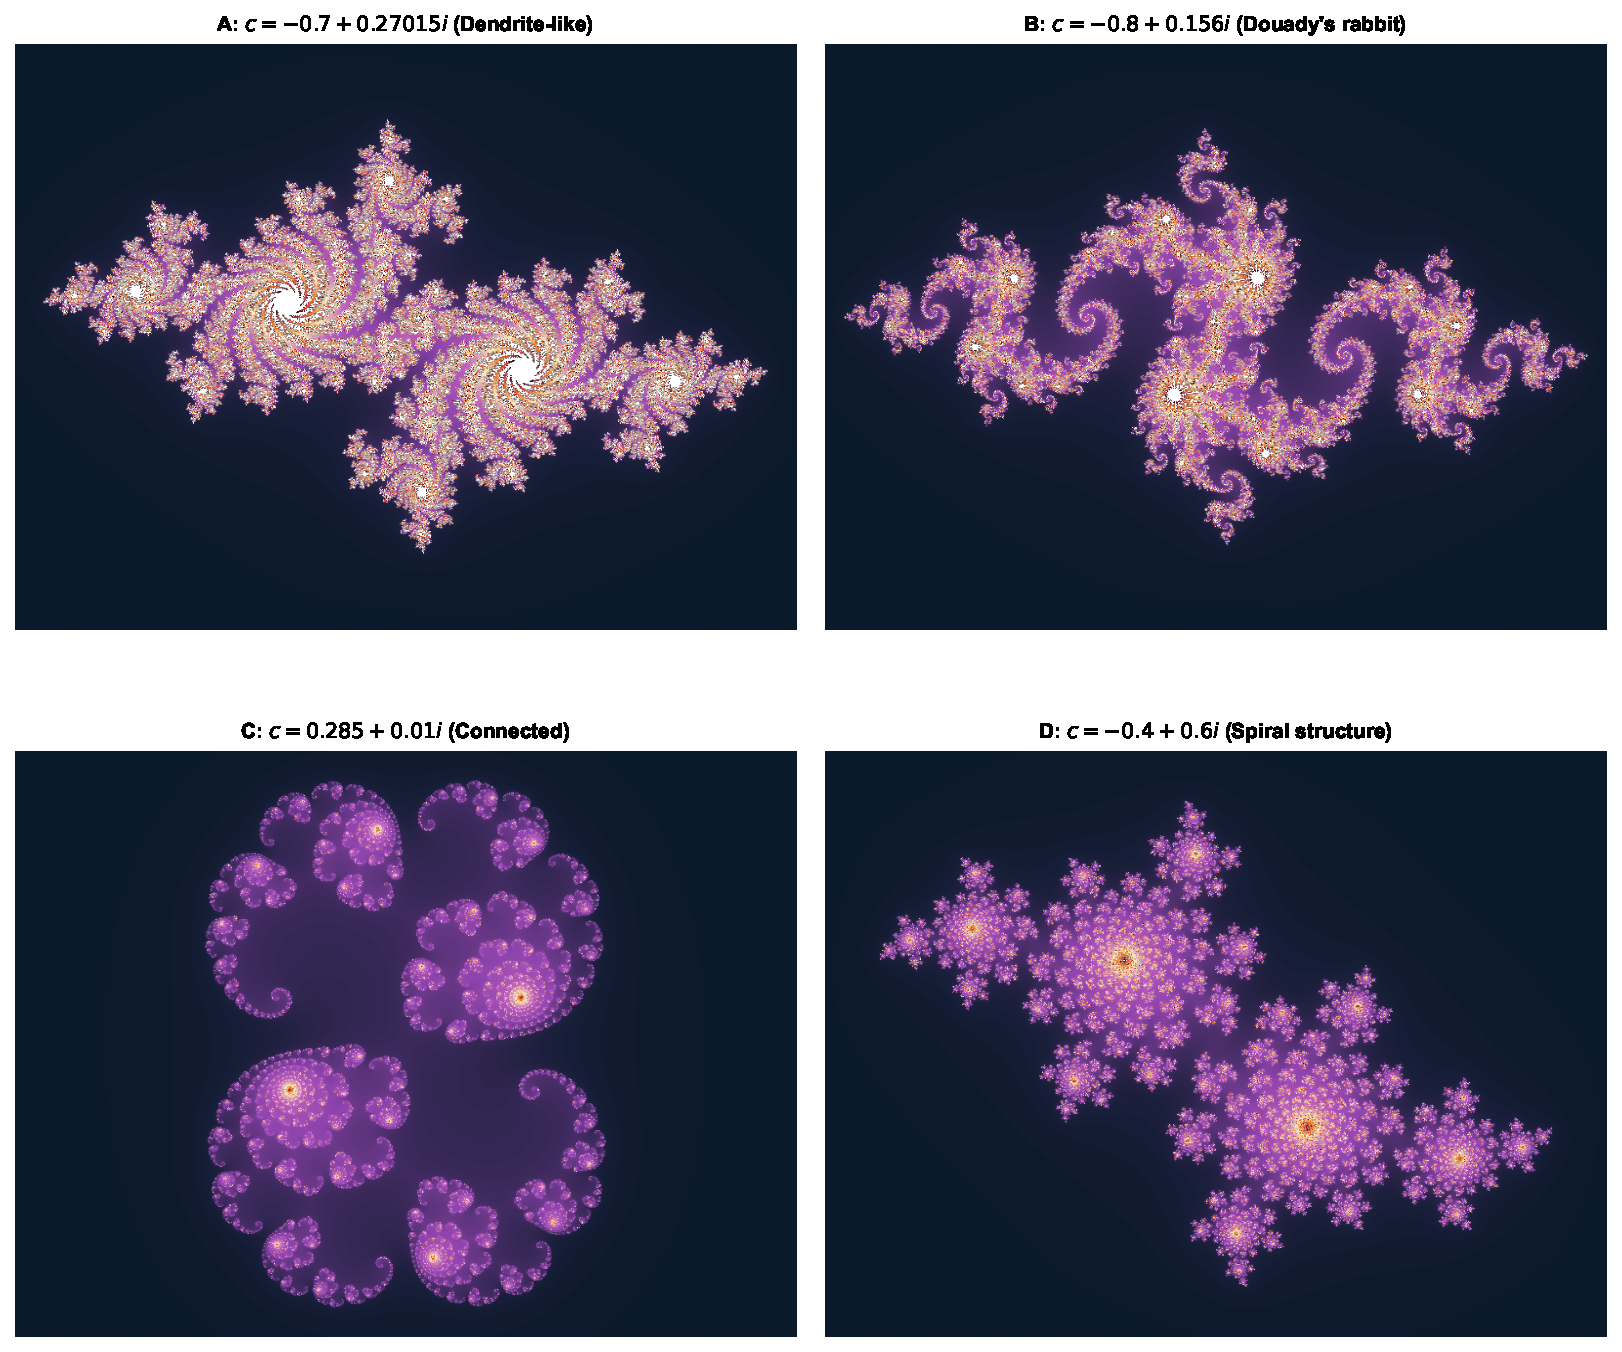
\includegraphics[width=\linewidth,height=4.4cm,keepaspectratio]{ch_fmh_julia_gallery.pdf}\\[1pt]
{\scriptsize\textcolor{MediumGray}{\textit{Galerie de mulțimi Julia pentru 4 valori ale $c$.}}}
\end{column}
\end{columns}
\quantlet{SFM\_ch\_fmh\_fractals: julia}{https://github.com/danpele/SFM/tree/main/Quantlets/SFM_ch_fmh}
\end{cminipage}
\end{frame}

\begin{frame}[shrink=15]{A3. Galerie: fractali în natură și în matematică}
\begin{cminipage}{0.96\textwidth}
\begin{columns}[T]
\begin{column}{0.32\textwidth}
\centering

\includegraphics[width=\linewidth,height=2.8cm,keepaspectratio]{ch_fmh_mandelbrot_full.pdf}\\[1pt]
{\tiny\textcolor{MediumGray}{Mulțimea Mandelbrot: $z\to z^2+c$}}
\end{column}
\begin{column}{0.32\textwidth}
\centering

\includegraphics[width=\linewidth,height=2.8cm,keepaspectratio]{ch_fmh_barnsley_fern.pdf}\\[1pt]
{\tiny\textcolor{MediumGray}{Feriga Barnsley (IFS)}}
\end{column}
\begin{column}{0.32\textwidth}
\centering
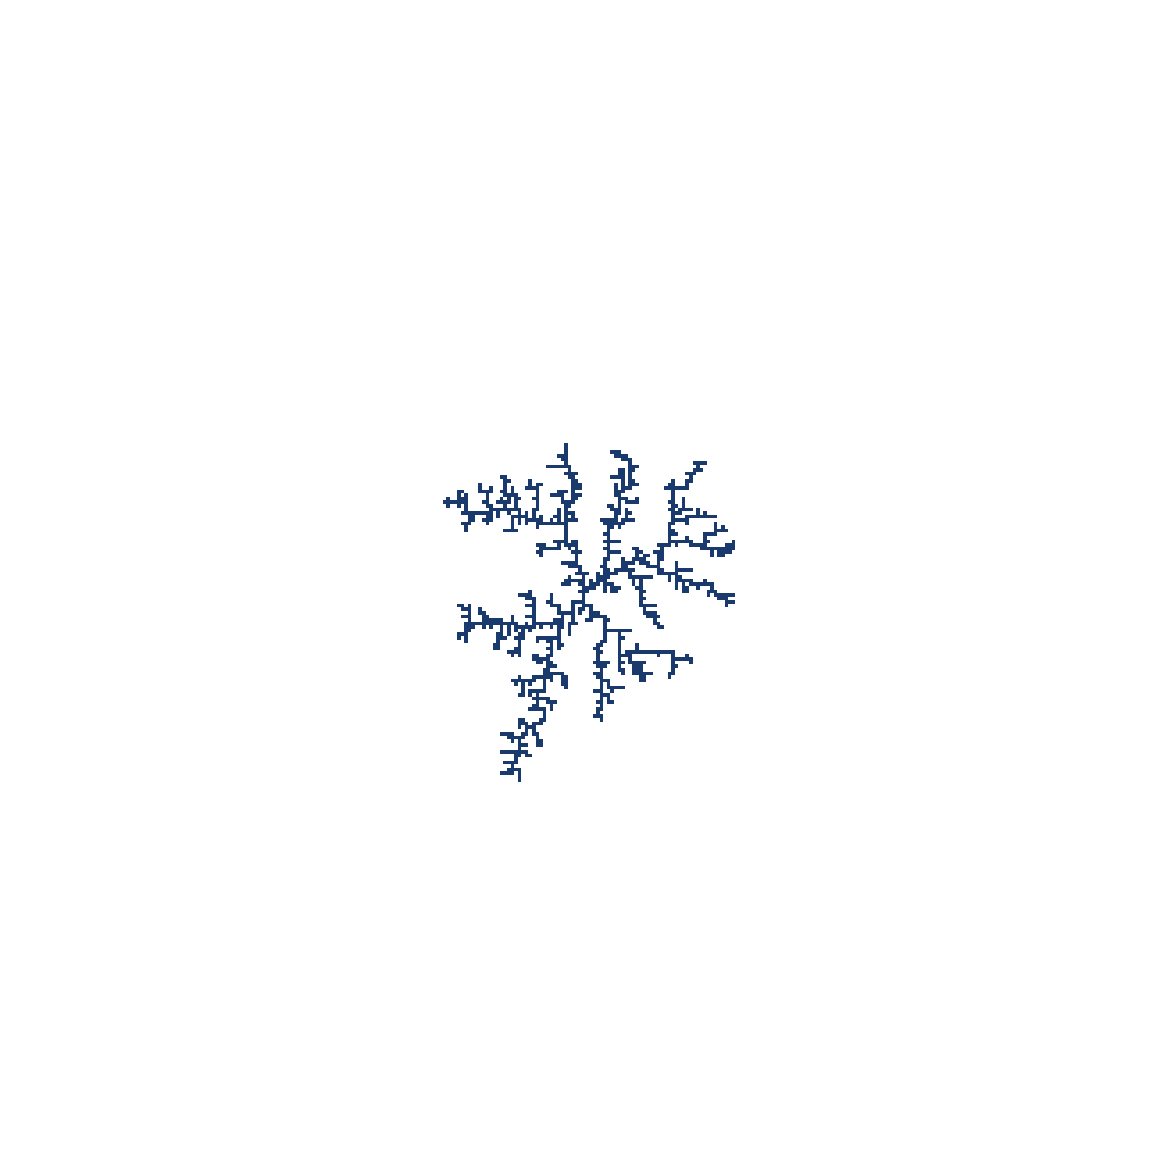
\includegraphics[width=\linewidth,height=2.8cm,keepaspectratio]{ch_fmh_dla.pdf}\\[1pt]
{\tiny\textcolor{MediumGray}{DLA --- fulger}}
\end{column}
\end{columns}
\vspace{0.1cm}
\begin{itemize}\setlength{\itemsep}{0pt}
    \item Fractali \textbf{deterministic}: Mandelbrot, Julia, Koch, Sierpinski, Cantor
    \item Fractali \textbf{naturali}: țărmuri, nori, copaci, sisteme circulatorii, fulger (DLA)
    \item Fractali \textbf{stocastici}: fBm, fGn, MMAR; cascade multiplicative
    \item \textbf{Mesaj}: structuri fractale apar peste tot --- inclusiv în piețele financiare
\end{itemize}
\quantlet{SFM\_ch\_fmh\_fractals + extra}{https://github.com/danpele/SFM/tree/main/Quantlets/SFM_ch_fmh}
\end{cminipage}
\end{frame}

\begin{frame}[shrink=15]{A4. Dimensiuni alternative: Hausdorff, informație, corelație}
\begin{cminipage}{0.95\textwidth}
\begin{itemize}\setlength{\itemsep}{1pt}
    \item Există mai multe variante de dimensiune fractală:
    \begin{itemize}\setlength{\itemsep}{0pt}
        \item Hausdorff $D_H$ --- standard riguros, dificil numeric
        \item Box-counting $D_{\text{box}}$ --- standardul empiric
        \item Similaritate $D_S$ --- pentru IFS auto-similare exact
        \item Informație $D_I$, corelație $D_C$, $q$-dimensiune $D_q$ --- multifractali
    \end{itemize}
    \item Pentru \textbf{monofractali}: $D_H=D_{\text{box}}=D_q$ (toate coincid)
    \item Pentru \textbf{multifractali}: $D_q$ depinde de $q$ $\Rightarrow$ se obține un \textbf{spectru de dimensiuni}
\end{itemize}
\vspace{0.1cm}
\begin{exampleblock}{Verificare iterativă: Cantor}
\begin{itemize}\setlength{\itemsep}{0pt}
    \item Box-counting: numărăm intervale de lungime $3^{-k}$ care acoperă $C_k$ $\Rightarrow N_k=2^k$
    \item $D=\lim_k\log(2^k)/\log(3^k)=\log 2/\log 3$ \checkmark coincide cu $D_S$
\end{itemize}
\end{exampleblock}
\end{cminipage}
\end{frame}

%-----------------------------------------------------------------------------
\section*{B. Metode avansate de estimare [APPENDIX OPȚIONAL]}
%-----------------------------------------------------------------------------

\begin{frame}[shrink=15]{B1. Alegerea parametrului $q$ în R/S Lo}
\begin{cminipage}{0.95\textwidth}
\begin{block}{Cum alegem $q$ (numărul de decalaje Newey--West)?}
\begin{itemize}\setlength{\itemsep}{0pt}
    \item Andrews (1991): $q^*=\lfloor (3T/2)^{1/3}\cdot(2\hat\rho/(1-\hat\rho^2))^{2/3}\rfloor$
    \item Aproximare: $q\approx \text{int}[4(T/100)^{2/9}]$ pentru $T<2000$
    \item Practic: $T=1000\Rightarrow q\approx 6$; $T=5000\Rightarrow q\approx 8$
\end{itemize}
\end{block}
\begin{exampleblock}{Caz tipic: BVB (BET, $T\approx 5000$)}
\begin{itemize}\setlength{\itemsep}{0pt}
    \item $q=8$, $R(n)=R$ obișnuit, $\sigma_n(8)$ corectat Newey--West
    \item $Q_n/\sqrt n\approx 2{,}3>1{,}862$ $\Rightarrow$ respingem $H_0:H=1/2$
    \item Concluzie: BET prezintă \textbf{memorie lungă}, nu doar dependență pe termen scurt
\end{itemize}
\end{exampleblock}
\begin{alertblock}{Avertisment}
\begin{itemize}\setlength{\itemsep}{0pt}
    \item Lo R/S detectează adesea sub-cantitativ memoria lungă (test conservator)
    \item Combinați cu DFA, GPH și Whittle pentru robustețe
\end{itemize}
\end{alertblock}
\end{cminipage}
\end{frame}

\begin{frame}[shrink=15]{B2. DFA: exemplu numeric pe serie scurtă}
\begin{cminipage}{0.95\textwidth}
\begin{exampleblock}{Date}
\begin{itemize}\setlength{\itemsep}{0pt}
    \item Aceeași serie ca la R/S: $x=\{0{,}5;\,-0{,}3;\,0{,}8;\,-0{,}2;\,0{,}6;\,-0{,}1;\,0{,}4;\,-0{,}7\}$
    \item Mărime segment: $n=4$ (două segmente: $\{Y_1,\ldots,Y_4\}$ și $\{Y_5,\ldots,Y_8\}$)
    \item Eliminare liniară a trendului (DFA-1)
\end{itemize}
\end{exampleblock}
\begin{itemize}\setlength{\itemsep}{0pt}
    \item \textbf{Pasul 1}: profilul $Y_k$ (calculat la R/S)
    \begin{itemize}\setlength{\itemsep}{0pt}
        \item $Y=\{0{,}375;\,-0{,}050;\,0{,}625;\,0{,}300;\,0{,}775;\,0{,}550;\,0{,}825;\,0\}$
    \end{itemize}
    \item \textbf{Pasul 2}: pe segmentul 1 ($k=1,\ldots,4$): regresie liniară $\hat Y_k=a_1+b_1 k$
    \begin{itemize}\setlength{\itemsep}{0pt}
        \item OLS dă $\hat a_1\approx 0{,}1875$, $\hat b_1\approx 0{,}075$
        \item Reziduuri: $Y_k-\hat Y_k$
    \end{itemize}
    \item \textbf{Pasul 3}: idem segmentul 2; calculăm suma pătratelor reziduurilor
    \item \textbf{Pasul 4}: $F(4)=\sqrt{(\sum r_k^2)/N}$
    \item \textbf{Pasul 5}: repetă pentru $n=2,4,8$ și aplică OLS pe $\log F(n)$ vs $\log n$ $\to$ panta $=\hat H$
    \item \textbf{Notă}: $n=4$ e prea mic pentru o estimare stabilă; pe date reale e nevoie de cel puțin 200--500 puncte
\end{itemize}
\end{cminipage}
\end{frame}

\begin{frame}[shrink=15]{B3. DFA-1, DFA-2, DFA-3: ordinul eliminării trendului}
\begin{cminipage}{0.95\textwidth}
\begin{itemize}\setlength{\itemsep}{2pt}
    \item \textbf{Construcție}
    \begin{itemize}\setlength{\itemsep}{0pt}
        \item DFA-$m$ elimină trenduri polinomiale de grad $\leq m$
        \item Exponent valid în $\alpha\in(0,m+1)$
    \end{itemize}
    \item \textbf{Diagnostic și recomandare}
    \begin{itemize}\setlength{\itemsep}{0pt}
        \item Punct de tranziție: $F(n)\sim n^{\alpha_1}$ pentru $n<n^*$, $\sim n^{\alpha_2}$ pentru $n>n^*$ $\Rightarrow$ regimuri multiple
        \item Pentru randamente bursiere: \textbf{DFA-1} sau \textbf{DFA-2}
    \end{itemize}
\end{itemize}
\vspace{0.1cm}
\renewcommand{\arraystretch}{1.2}
\centering
\small
\begin{tabular}{lll}
\toprule
\textbf{Variabilă} & \textbf{DFA recomandat} & \textbf{Motiv} \\
\midrule
Randamente staționare ($r_t$) & DFA-1 & Eliminarea liniară a trendului e suficientă \\
Volatilitate ($|r_t|$, $r_t^2$) & DFA-1 sau DFA-2 & Posibil trend lent \\
Prețuri nestaționare ($\ln P_t$) & DFA-2 sau DFA-3 & Trenduri polinomiale \\
Volume cu sezonalitate & DFA-3 & Trend ciclic \\
\bottomrule
\end{tabular}
\end{cminipage}
\end{frame}

\begin{frame}[shrink=15]{B4. Comparație metode: R/S, Lo, DFA, MFDFA, GPH, Whittle, wavelet}
\begin{cminipage}{0.95\textwidth}
\renewcommand{\arraystretch}{1.2}
\centering
\small
\begin{tabular}{llll}
\toprule
\textbf{Metodă} & \textbf{Robust trenduri?} & \textbf{Multifractal?} & \textbf{Recomandare} \\
\midrule
R/S clasic (Hurst 1951) & Nu & Nu & Educațional \\
R/S modificat (Lo 1991) & Parțial & Nu & Test formal $H=0{,}5$ \\
DFA-1 (Peng 1994) & Da (liniar) & Nu & \textbf{Standard} pentru randamente \\
DFA-2/3 & Da (polinom.) & Nu & Pentru prețuri nestaționare \\
MFDFA (Kantelhardt 2002) & Da & Da & Spectru $h(q),\,f(\alpha)$ \\
GPH (Geweke--Porter-Hudak, 1983) & Nu & Nu & Periodogramă, semi-param \\
Whittle & Da & Nu & Cel mai eficient asimptotic \\
Wavelet (WTMM) & Da & Da & Cea mai bună acuratețe \\
\bottomrule
\end{tabular}
\vspace{0.15cm}
\begin{exampleblock}{Combinație recomandată}
\begin{itemize}\setlength{\itemsep}{0pt}
    \item DFA-1 (principal) + Variance Ratio (test formal $H=0{,}5$)
    \item R/S Lo (robustețe) + MFDFA (multifractal, dacă există resurse de calcul)
\end{itemize}
\end{exampleblock}
\end{cminipage}
\end{frame}

\begin{frame}[shrink=15]{B5. Bai--Perron: detectarea punctelor de ruptură}
\begin{cminipage}{0.95\textwidth}
\begin{block}{Procedura Bai \& Perron (1998, 2003)}
\begin{itemize}\setlength{\itemsep}{0pt}
    \item Dat $\hat H_t$ pe fereastră mobilă, testăm dacă există $m$ schimbări structurale la momentele $t_1<\cdots<t_m$
    \item Estimare prin minimizarea sumei pătratelor pe segmente
    \item Test secvențial $\sup F$: $H_0$ niciun punct de ruptură vs.\ $H_1$ exact $m$ rupturi
\end{itemize}
\end{block}
\begin{exampleblock}{Aplicație tipică pe S\&P 500 (2000--2024)}
\begin{itemize}\setlength{\itemsep}{0pt}
    \item Detectează 3--4 rupturi majore: 2008, 2011 (criza euro), 2020 (COVID), 2022 (inflație)
    \item Pe sub-intervalele stabile: $\hat H\approx 0{,}55$
    \item În jurul punctelor de ruptură: $\hat H$ scade rapid
\end{itemize}
\end{exampleblock}
\begin{alertblock}{Mesaj metodologic}
\begin{itemize}\setlength{\itemsep}{0pt}
    \item \textbf{Întotdeauna} verificăm rupturile înainte de a interpreta $\hat H$ pe perioade lungi
    \item Granger \& Ding (1996): rupturile pot da $\hat H>0{,}5$ \textbf{spurios}
    \item Reflex bun: $\hat H_t$ pe fereastră mobilă + Bai--Perron + DFA pe sub-intervale
\end{itemize}
\end{alertblock}
\end{cminipage}
\end{frame}

%-----------------------------------------------------------------------------
\section*{C. Modele stocastice și evaluarea opțiunilor [APPENDIX OPȚIONAL]}
%-----------------------------------------------------------------------------

\begin{frame}[shrink=15]{C1. Davies--Harte: simularea exactă a fBm}
\begin{cminipage}{0.95\textwidth}
\begin{block}{Algoritmul Davies--Harte (1987)}
\begin{enumerate}\setlength{\itemsep}{1pt}
    \item Calculăm \textbf{covarianța} fGn pe lag-uri $0,1,\ldots,N-1$:
    \[ \gamma(k)=\tfrac12(|k+1|^{2H}-2|k|^{2H}+|k-1|^{2H}) \]
    \item Construim \textbf{matricea circulantă} $C$ de mărime $2N\times 2N$ cu prima linie $(\gamma(0),\gamma(1),\ldots,\gamma(N-1),0,\gamma(N-1),\ldots,\gamma(1))$
    \item Aplicăm FFT $\Rightarrow$ valorile proprii $\Lambda_k$ (pozitive dacă $H<1$)
    \item Generăm $Z\sim\mathcal{CN}(0,I)$; calculăm $W=F^*\sqrt\Lambda Z$ via inverse FFT
    \item Primele $N$ componente ale $\text{Re}(W)$ = traiectorie fGn; cumulând $\Rightarrow$ fBm
\end{enumerate}
\end{block}
\begin{exampleblock}{De ce este important}
\begin{itemize}\setlength{\itemsep}{0pt}
    \item Complexitate: $O(N\log N)$ vs $O(N^2)$ pentru factorizarea Cholesky
    \item Pentru $N=10^6$: Cholesky $\sim$ ore; Davies--Harte $\sim$ secunde
    \item Folosit în industrie pentru Monte Carlo cu fBm (evaluarea opțiunilor sub modelul rough Heston)
\end{itemize}
\end{exampleblock}
\end{cminipage}
\end{frame}

\begin{frame}[shrink=15]{C2. Cascada multiplicativă binomială}
\begin{cminipage}{0.95\textwidth}
\begin{columns}[T]
\begin{column}{0.55\textwidth}
\begin{block}{Construcție iterativă (Mandelbrot, 1974)}
\begin{itemize}\setlength{\itemsep}{0pt}
    \item Pornim de la măsura uniformă pe $[0,1]$ cu masă 1
    \item La fiecare pas, fiecare interval se împarte în 2 jumătăți cu mase $m_0,m_1$ (cu $m_0+m_1=1$)
    \item După $k$ pași: $2^k$ intervale, fiecare cu masă $m_0^j m_1^{k-j}$
\end{itemize}
\end{block}
\begin{exampleblock}{Proprietăți}
\begin{itemize}\setlength{\itemsep}{0pt}
    \item Generează un \textbf{multifractal} (nu monofractal)
    \item Spectrul $f(\alpha)$ are formă de clopot
    \item Modelează volatilitatea cu intermitență
\end{itemize}
\end{exampleblock}
\end{column}
\begin{column}{0.42\textwidth}
\centering
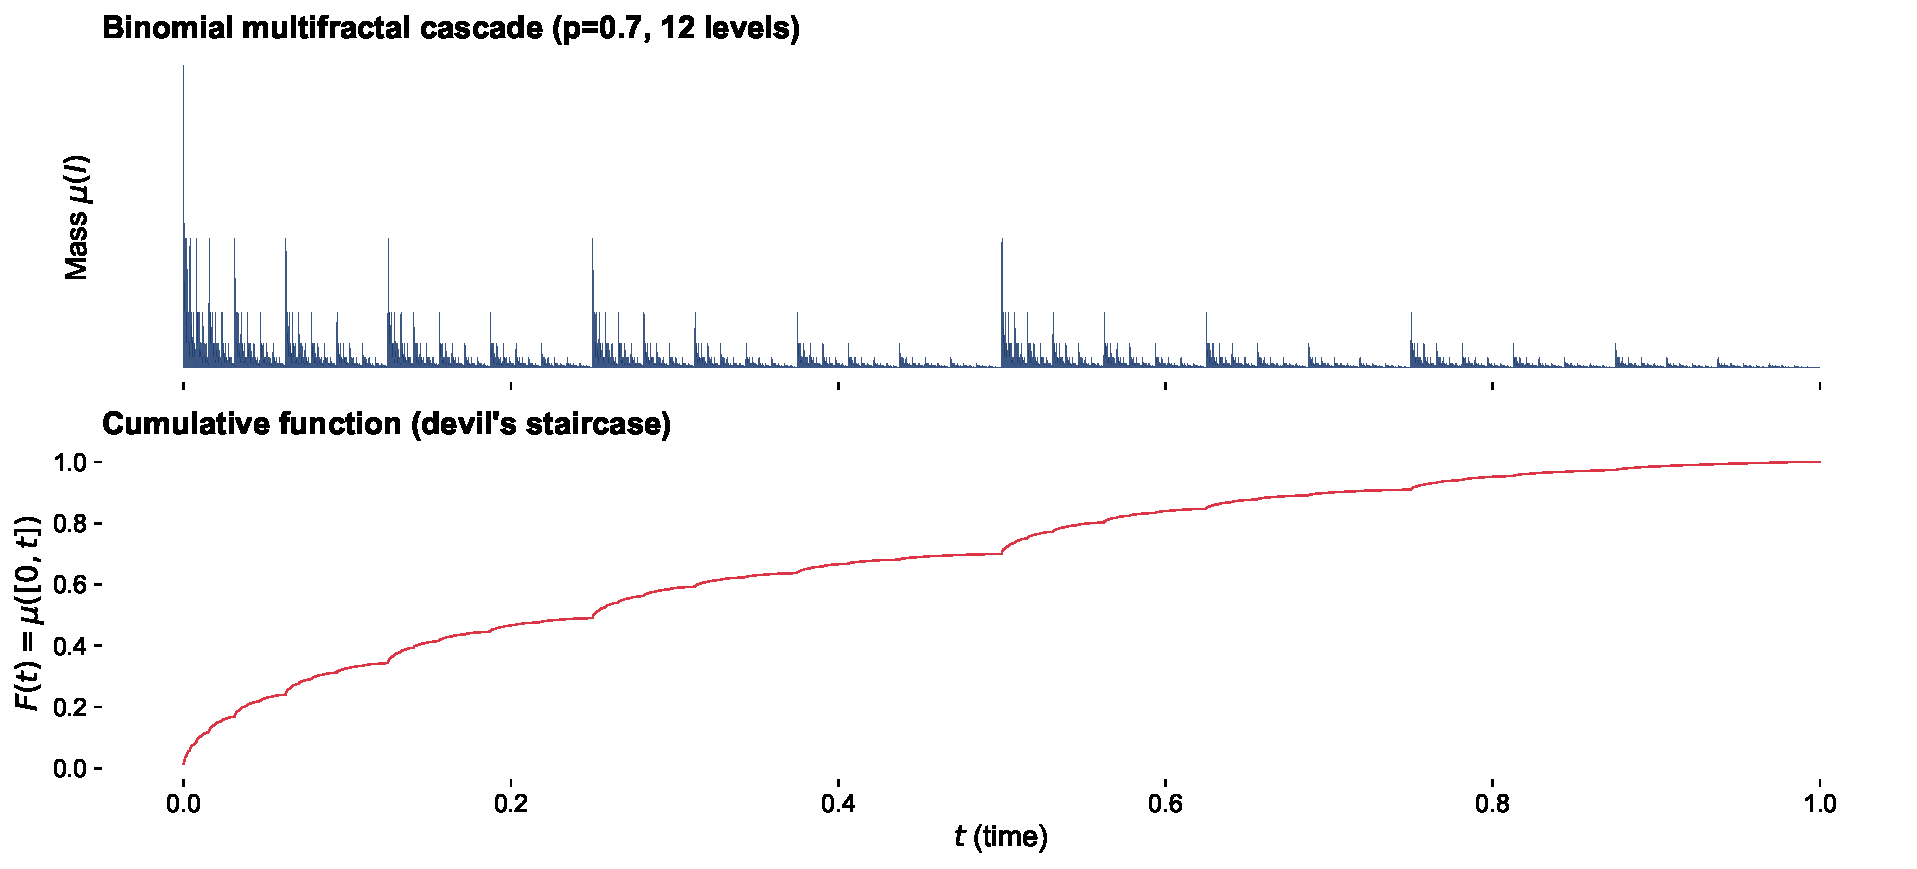
\includegraphics[width=\linewidth,height=4.4cm,keepaspectratio]{ch_fmh_multi_cascade.pdf}\\[1pt]
{\scriptsize\textcolor{MediumGray}{\textit{Cascadă multiplicativă binomială: 5 iterații.}}}
\end{column}
\end{columns}
\quantlet{SFM\_ch\_fmh\_extra: multi\_cascade}{https://github.com/danpele/SFM/tree/main/Quantlets/SFM_ch_fmh}
\end{cminipage}
\end{frame}

\begin{frame}[shrink=15]{C3. MMAR (\textit{Multifractal Model of Asset Returns})}
\begin{cminipage}{0.95\textwidth}
\begin{itemize}\setlength{\itemsep}{1pt}
    \item \textbf{Construcție} (Mandelbrot, Fisher, Calvet, 1997)
    \begin{itemize}\setlength{\itemsep}{0pt}
        \item Log-prețul: $\ln P(t)=B_H(\theta(t))$
        \item $\theta(t)=\int_0^t\mu(ds)$ = \textbf{timp de tranzacționare multifractal}
        \item Idee: timpul calendaristic $\neq$ timpul economic
    \end{itemize}
    \item \textbf{Avantaje}
    \begin{itemize}\setlength{\itemsep}{0pt}
        \item Modelare unificată a 4 fapte stilizate: cozi grele, aglomerarea volatilității, memorie lungă, multifractalitate
    \end{itemize}
    \item \textbf{Limitări și extensii}
    \begin{itemize}\setlength{\itemsep}{0pt}
        \item Critică: estimare dificilă; greu de simulat exact
        \item Variantă mai tratabilă: \textbf{MSM} (Markov-Switching Multifractal, Calvet \& Fisher 2004)
    \end{itemize}
\end{itemize}
\vspace{0.1cm}
\begin{exampleblock}{De ce MMAR este important}
\begin{itemize}\setlength{\itemsep}{0pt}
    \item Permite \textbf{modelarea simultană} a celor 4 fapte stilizate într-un singur cadru continuu (cf.\ Calvet \& Fisher, 2002, 2004)
    \item Prognoza multifractală e competitivă față de GARCH pe orizonturi medii (5--22 zile)
\end{itemize}
\end{exampleblock}
\end{cminipage}
\end{frame}

\begin{frame}[shrink=15]{C4. FIGARCH (\textit{Fractionally Integrated GARCH}): volatilitate cu memorie lungă}
\begin{cminipage}{0.95\textwidth}
\begin{itemize}\setlength{\itemsep}{1pt}
    \item \textbf{Definiție FIGARCH (Baillie--Bollerslev--Mikkelsen, 1996)}
    \begin{itemize}\setlength{\itemsep}{0pt}
        \item Fractionally Integrated GARCH: GARCH(1,1) cu diferențiere fracționară
        \[
            (1-L)^d\varepsilon_t^2=\omega+\beta(L)v_t,\quad d\in(0,1/2)
        \]
        \item Surprinde: $\Corr(\varepsilon_t^2,\varepsilon_{t-k}^2)\sim k^{2d-1}$ (decadere hiperbolică)
    \end{itemize}
    \item \textbf{Comparație}
    \begin{itemize}\setlength{\itemsep}{0pt}
        \item GARCH(1,1): decadere exponențială $\Rightarrow$ subestimează aglomerarea volatilității pe orizont mediu
        \item IGARCH ($d=1$): decadere infinită $\Rightarrow$ supraestimează
        \item FIGARCH ($0<d<1/2$): decadere hiperbolică $\Rightarrow$ corect
    \end{itemize}
\end{itemize}
\begin{exampleblock}{Implementare}
\begin{itemize}\setlength{\itemsep}{0pt}
    \item Python: \texttt{arch} (Sheppard, MIT License)
    \item Aplicabil oricărei serii cu memorie lungă în volatilitate (S\&P 500, BTC, FX)
\end{itemize}
\end{exampleblock}
\end{cminipage}
\end{frame}

\begin{frame}[shrink=15]{C5. HAR (\textit{Heterogeneous AutoRegressive}): cascadă pe orizonturi (Corsi, 2009)}
\begin{cminipage}{0.95\textwidth}
\begin{block}{HAR-RV (Heterogeneous AutoRegressive Realized Volatility)}
\[
    RV_{t+1}=\beta_0+\beta_d\,RV_t^{(d)}+\beta_w\,RV_t^{(w)}+\beta_m\,RV_t^{(m)}+\varepsilon_{t+1}
\]
\begin{itemize}\setlength{\itemsep}{0pt}
    \item $RV^{(d)}$ = volatilitate realizată pe 1 zi
    \item $RV^{(w)}$ = pe 5 zile (săptămână)
    \item $RV^{(m)}$ = pe 22 zile (lună)
\end{itemize}
\end{block}
\begin{exampleblock}{De ce HAR este ,,sora FMH''}
\begin{itemize}\setlength{\itemsep}{0pt}
    \item Conceptual: investitorii cu \textbf{orizonturi diferite} contribuie la formarea volatilității
    \item Operațional: simplu de estimat (OLS), surprinde memoria lungă fără diferențiere fracționară
    \item Empiric: HAR este competitiv (și frecvent superior) față de GARCH la prognoza pe orizonturi de 5--22 zile (Andersen et~al.\ 2007; Corsi 2009)
\end{itemize}
\end{exampleblock}
\end{cminipage}
\end{frame}

\begin{frame}[shrink=15]{C6. Evaluarea opțiunilor sub fBm}
\begin{cminipage}{0.95\textwidth}
\begin{itemize}\setlength{\itemsep}{2pt}
    \item \textbf{Problemă fundamentală}
    \begin{itemize}\setlength{\itemsep}{0pt}
        \item fBm pur \textbf{nu este semimartingală} (Rogers, 1997) $\Rightarrow$ permite arbitraj
        \item Black--Scholes nu se aplică direct
    \end{itemize}
    \item \textbf{Soluții moderne}
    \begin{itemize}\setlength{\itemsep}{0pt}
        \item \textbf{fBm mixt} (Cheridito 2001): combinație fBm + browniană standard
        \item \textbf{Calcul Wick--Itô}: integrală stocastică modificată
        \item \textbf{Volatilitate ,,rough''} (Gatheral, Jaisson, Rosenbaum, 2018): volatilitatea are $H\approx 0{,}1$
    \end{itemize}
    \item \textbf{Modelul rough Heston} (El Euch \& Rosenbaum, 2019)
    \begin{itemize}\setlength{\itemsep}{0pt}
        \item Surprinde mai bine ,,zâmbetul'' volatilității implicite pe orizonturi scurte
        \item Calibrare empirică: $H\in[0{,}05;\,0{,}15]$ pentru S\&P 500
    \end{itemize}
\end{itemize}
\begin{alertblock}{Paradox aparent}
\begin{itemize}\setlength{\itemsep}{0pt}
    \item Prețurile au $H\approx 0{,}55$--$0{,}65$ (persistent)
    \item Volatilitatea are $H\approx 0{,}1$ (puternic anti-persistentă, ,,rough'')
    \item Două regimuri Hurst diferite $\Rightarrow$ multifractalitatea (MMAR, MSM, volatilitatea ,,rough'') este un cadru natural
\end{itemize}
\end{alertblock}
\end{cminipage}
\end{frame}

\end{document}
